\documentclass[12pt, a4paper, onecolumn, oneside, final]{report}

% Load konfigurasi LaTeX untuk tipe laporan thesis
\usepackage{src/unpam}
\usepackage{enumitem}
\usepackage{array}
\usepackage{graphics}
\usepackage{microtype}
\usepackage{adjustbox}
\usepackage[numbers]{natbib}
\usepackage{xcolor} % in your preamble


% * Revisi Rumusan hasil rumusan di bab 4
% * Revisi terkait penulisan implementasi yang ada di github masukan di skripsi
% * Penjelasan terkait hasil implementasi service pada bab 4 (color, frontend, auth)

% * Tambahkan testing pada sisi service seperti (jaringan, waktu (speed))
% * gambar dan tabel dirujuk semua lalu diberikan border
% * dalam subbab perlu a,b,c bukan 1,2,3 (contoh di halaman 13)
% * gambar dijelaskan why nya
% * bab 2 tolong ditambahkan literatur nya dan ditampilkan penelitian terdahulu


% format penulisan
% * Penulisan sub bab harus melihat penjelasan dan kalimat yang diutarakan
% * perlu diperbaiki secara serius dalam uji microservice
% * uji fungsionalitas terhadap microservice pada bab 4



% %%%%%%%%%%%%%%%%%%%%%%%%%%%%%%%%%%%%%%%%%%%%%%%%%%%%%%%%%%
% %%%%%%%%%%%%%%%%%%%%%%%%%%%%%%%%%%%%%%%%%%%%%%%%%%%%%%%%%%
% Variabel baru untuk menyimpan nomor halaman
\newcounter{originalpagenumber}
% Awal bagian penulisan laporan
\begin{document}

%
% Hyphenation untuk Indonesia 
%
% @author  Enggar Alfianto
% @version 1.00
% 
% Tambahkan cara pemenggalan kata-kata yang salah dipenggal secara otomatis 
% oleh LaTeX. Jika kata tersebut dapat dipenggal dengan benar, maka tidak 
% perlu ditambahkan dalam berkas ini. Tanda pemenggalan kata menggunakan 
% tanda '-'; contoh:
% menarik
%   --> pemenggalan: me-na-rik
%

\hyphenation{
    % alphabhet A
    a-na-li-sa a-tur
    a-pli-ka-si
    a-na-li-tik
    % alphabhet B
    ba-ngun-an
    be-be-ra-pa
    ber-ge-rak
    ber-ke-lan-jut-an
    ber-pe-nga-ruh
    bim-bing-an
    % alphabhet C
    ca-ri
    % alphabhet D
    di-sim-pan di-pim-pin de-ngan da-e-rah di-ba-ngun da-pat di-nya-ta-kan
    di-sim-bol-kan di-pi-lih di-li-hat de-fi-ni-si
    di-rahmat-i
    di-identifi-kasi-kan
    di-re-pre-sen-ta-si-kan
    du-kung-an-nya
    % alphabhet E
    e-ner-gi eks-klu-sif
    % alphabhet F
    fa-si-li-tas
    fe-no-me-na
    % alphabhet G
    ga-bung-an ge-rak
    % alphabhet H
    ha-lang-an
    hamilton-nia-nya
    % alphabhet I
    % alphabhet J
    % alphabhet K
    ke-rapat-an
    ke-hi-lang-an
    ku-ning
    kompu-tasi
    kua-li-tas ka-me-ra ke-mung-kin-an ke-se-pa-ham-an
    % alphabhet L
    ling-kung-an
    % alphabhet M
    me-nge-luar-kan
    me-neng-ah
    mem-perhitung-kan
    mem-ban-ding-kan
    meng-a-tas-i me-mung-kin-kan me-nge-na-i me-ngi-rim-kan
    meng-u-bah meng-a-dap-ta-si me-nya-ta-kan mo-di-fi-ka-si
    meng-a-tur
    micro-service
    % alphabhet N
    nya-ta non-eks-klu-sif
    nano-tekno-logi
    % alphabhet O
    % alphabhet P
    pa-ling
    pe-nye-rap-an
    pe-ngon-trol
    pe-mo-del-an
    pe-ran  pe-ran-an-nya
    pem-ba-ngun-an pre-si-den pe-me-rin-tah prio-ri-tas peng-am-bil-an
    peng-ga-bung-an pe-nga-was-an pe-ngem-bang-an
    pe-nga-ruh pa-ra-lel-is-me per-hi-tung-an per-ma-sa-lah-an
    pen-ca-ri-an peng-struk-tur-an
    % alphabhet Q
    % alphabhet R
    ran-cang-an
    % alphabhet S
    si-mu-la-si sa-ngat
    se-bagai
    semi-konduktor
    % alphabhet T
    te-ngah
    ter-da-pat
    ter-selesai-kanya
    % alphabhet U
    % alphabhet V
    % alphabhet W
    % alphabhet X
    % alphabhet Y
    % alphabhet Z
    % special
}

% Sampul Laporan
\begin{titlepage}
    \begin{center}
        \onehalfspacing
        \large \bfseries \textit{Automatic Deployment}  Aplikasi berbasis \textit{Microservice} Pada Platform Kubernetes Dengan Metode \textit{Pull-Up} \\
        \vspace{1cm}
        \large Laporan Tugas Akhir \\
        \vspace{0.5cm}

        {\small \normalfont Diajukan Untuk Memenuhi\\
            Persyaratan Guna Meraih Gelar Sarjana\\
            Informatika Universitas Muhammadiyah Malang}
        \vspace{2cm}

        
\includegraphics[width=6cm]{figures/logo_umm.png}

        \vspace{1cm}
        \normalfont \normalsize Muhammad Zein Ihza Fahrozi \\
        \normalfont \normalsize 201810370311072 \\

        \vspace{1cm}
        \bfseries \normalsize Bidang Minat \\
        \normalfont \normalsize Rekayasa Perangkat Lunak

        \vspace{2.5cm}

        \normalsize PROGRAM STUDI TEKNIK INFORMATIKA FAKULTAS TEKNIK \\
        UNIVERSITAS MUHAMMADIYAH MALANG \\
        2021



    \end{center}

\end{titlepage}

\newpage

% Daftar isi, gambar, dan tabel
% Gunakan penomeran Romawi (i, ii, iii, ...) setelah bagian ini.
\pagenumbering{roman}

% Lembar Persetujuan
\phantomsection \addcontentsline{toc}{chapter}{LEMBAR PERSETEJUAN}
\chapter*{\uppercase{LEMBAR PERSETUJUAN}}
\vspace{1cm}

\begin{center}
    ``To Be Added Bismillah''
\end{center}

\newpage

% Lembar Pengesahan
\phantomsection \addcontentsline{toc}{chapter}{LEMBAR PENGESAHAN}
\chapter*{\uppercase{LEMBAR PENGESAHAN}}
\vspace{1cm}

\center ``To Be Added Bismillaah''

\newpage

% Lembar Pernyataan
\phantomsection \addcontentsline{toc}{chapter}{LEMBAR PERNYATAAN}
\chapter*{\uppercase{LEMBAR PERNYATAAN}}

\begin{center}
    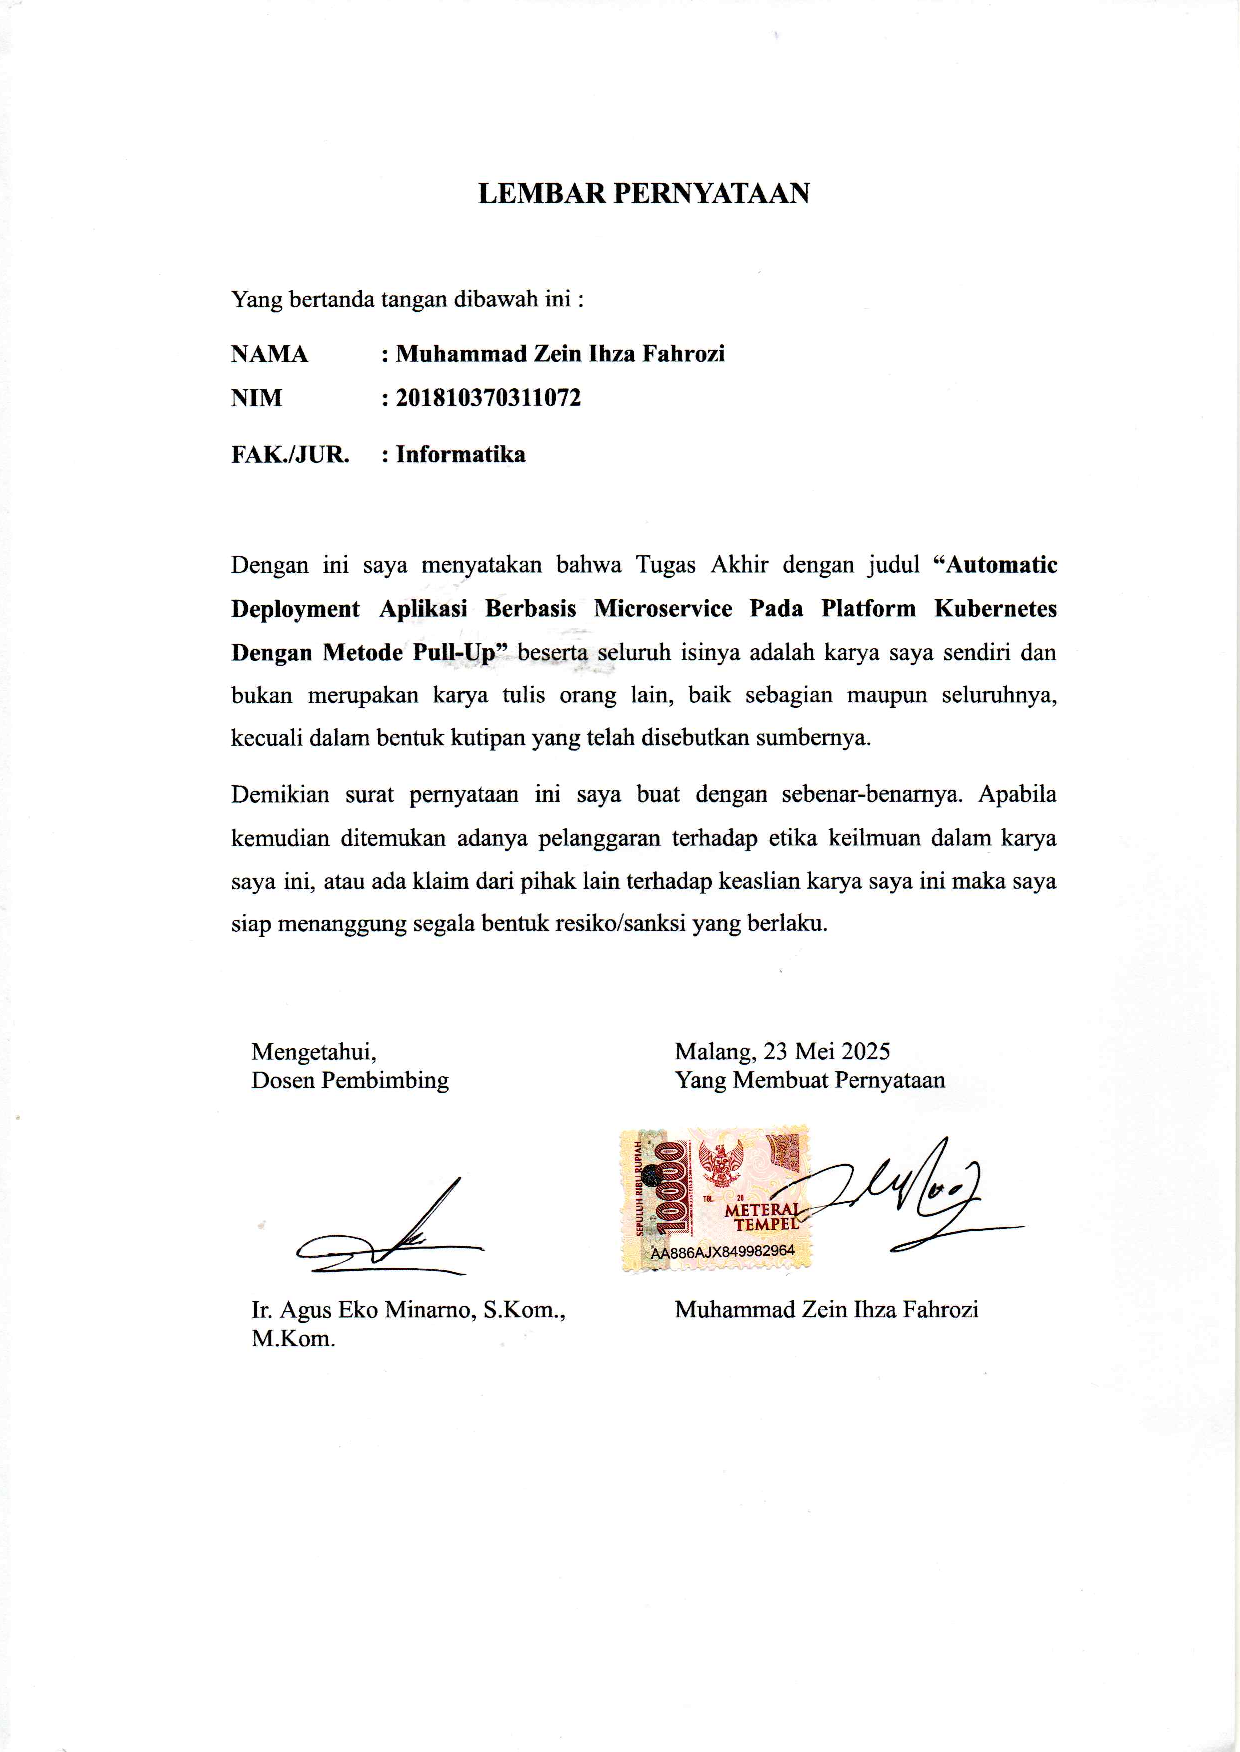
\includegraphics[width=\textwidth,page=1]{misc/lembar-pernyataan-scan.pdf}
\end{center}

\newpage


% Abstrak
%
% Halaman Abstract
\phantomsection \addcontentsline{toc}{chapter}{ABSTRAK}
\chapter*{ABSTRAK}

\begin{singlespace}
	\blindtext \\[20pt]
	Keywords: \textit{Information System, Testing Project}
\end{singlespace}

\newpage

\phantomsection \addcontentsline{toc}{chapter}{ABSTRACT}
\chapter*{ABSTRACT}

\begin{singlespace}
	\blindtext \\[20pt]
	Keywords: \textit{Information System, Testing Project}
\end{singlespace}

\newpage


% Lembar Persembahan
\phantomsection \addcontentsline{toc}{chapter}{LEMBAR PERSEMBAHAN}
\chapter*{\uppercase{LEMBAR PERSEMBAHAN}}
\vspace{1cm}

\begin{center}
    ``To Be Added Bismillah''
\end{center}

\newpage


\chapter*{\uppercase{KATA PENGANTAR}}
\vspace{1cm}

\begin{center}
    ``To Be Added Bismillah''
\end{center}

\newpage

% Daftar Isi
\vspace*{-2.5cm}
\tableofcontents
\phantomsection \addcontentsline{toc}{chapter}{DAFTAR ISI}
\clearpage
% Daftar Tabel
\vspace*{-2.5cm}
\listoftables
\phantomsection \addcontentsline{toc}{chapter}{DAFTAR TABEL}
\clearpage
% Daftar Gambar
\vspace*{-2.5cm}
\listoffigures
\phantomsection
\addcontentsline{toc}{chapter}{DAFTAR GAMBAR}
\clearpage

% Gunakan penomeran Arab (1, 2, 3, ...) setelah bagian ini.
\pagenumbering{arabic}

%
% Atur header dan footer dalam dokumen.
% 
\renewcommand{\headrulewidth}{0.0pt}
\fancyhf{}
\fancyhead[L]{}
\fancyhead[C]{}
% \fancyhead[R]{\thepage}
\fancyfoot[CO]{\thepage}
\renewcommand{\headrulewidth}{0.0pt}
\renewcommand{\footrulewidth}{0.0pt}
\pagestyle{fancy}

\onehalfspacing
\renewcommand{\chaptername}{BAB}
%-----------------------------------------------------------------------------%
\chapter{PENDAHULUAN}
%-----------------------------------------------------------------------------%
\vspace{4.5pt}
\setlength{\parskip}{0.5em}

\section{Latar Belakang} \label{sec:latar_belakang}
Sebelum digunakan oleh pengguna secara luas, sebuah perangkat lunak perlu
melalui proses \textit{deployment} terlebih dahulu. \textit{Deployment}
perangkat lunak dapat didefinisikan sebagai akuisisi dan eksekusi sebuah
perangkat lunak. Proses ini biasanya dilakukan oleh seorang software deployer
atau yang lebih dikenal saat ini sebagai SRE (site reliability engineer)
\cite{Lyu2007}. Dengan demikian, \textit{deployment} dapat dikatakan sebagai
aktivitas pasca-produksi sebuah perangkat lunak sebelum digunakan oleh
konsumen. Proses \textit{deployment} perangkat lunak terdiri dari beberapa
tahapan yang saling berhubungan, seperti proses rilis perangkat lunak,
instalasi perangkat lunak ke dalam environment eksekusi, dan aktivasi perangkat
lunak \cite{Carzaniga1998}.

Pada saat melakukan \textit{deployment} sebuah sistem perangkat lunak, beberapa
aspek perlu diperhatikan, seperti sub-komponen yang dibutuhkan atau
\textit{package external}, serta \textit{resource} (hardware). Untuk melakukan
\textit{deployment} sub-komponen ini, dibutuhkan sebuah konfigurasi yang
mendeskripsikan versi sub-komponen yang digunakan oleh perangkat lunak. Dengan
bahasa modern sekarang, konfigurasi sub-komponen yang digunakan oleh main
perangkat lunak biasanya sudah dapat dihasilkan secara otomatis, contohnya
adalah; \textit{go modules} \cite{go_mod} dalam bahasa Golang,
\textit{requirement file} \cite{requirementPython} dalam bahasa Python, atau
file \textit{RubySpec} \cite{rubySpec} pada bahasa Ruby.
\par

Terdapat beberapa karakteristik fundamental dalam \textit{deployment} perangkat
lunak yang diidentifikasi oleh Alan Dearle \cite{Dearle2007}, yaitu:

\textbf{\textit{Release}} merupakan tahap penghubung antara proses \textit{deployment} dengan pengembangan perangkat lunak. Tahap ini mencakup seluruh operasi yang diperlukan untuk mempersiapkan sistem sebelum diserahkan kepada pengguna akhir. Aktivitas \textit{release} juga meliputi penentuan sumber daya (\textit{resource}) yang dibutuhkan agar sistem dapat beroperasi dengan optimal pada \textit{environment} yang ditargetkan.

Selanjutnya dilakukan \textit{packaging} terhadap sistem perangkat lunak.
\textit{Package} yang dihasilkan harus memuat seluruh komponen yang dibutuhkan,
termasuk deskripsi sistem, \textit{dependencies} eksternal, prosedur
\textit{deployment}, serta informasi relevan lainnya yang diperlukan untuk
menjalankan sistem pada \textit{environment} tujuan.

\textbf{\textit{Installation}} merupakan tahap persiapan sebelum aktivasi sistem. \textbf{\textit{Activation}} merupakan proses eksekusi perangkat lunak pada waktu tertentu, yang dapat dilakukan melalui antarmuka grafis (\textit{graphical user interface}) atau sebagai layanan latar belakang (\textit{daemon process}).

\textbf{\textit{Updating}} adalah proses penggantian komponen perangkat lunak yang terinstal dengan versi yang lebih baru. Adapun \textbf{\textit{Undeployment}} atau yang dikenal juga sebagai \textit{deinstallation}, merupakan proses penghapusan perangkat lunak yang terinstal dari suatu sistem.
\par
Menurut penelitian yang dilakukan oleh Mockus dkk. \cite{Mockus2005}, kualitas
\textit{deployment} suatu perangkat lunak merupakan salah satu faktor utama
yang mempengaruhi persepsi konsumen terhadap kualitas keseluruhan perangkat
lunak tersebut. Hal senada diungkapkan oleh Jansen dan Brinkkemper
\cite{Jansen2006} yang menyatakan bahwa kelancaran proses \textit{deployment}
merupakan aspek esensial dalam meningkatkan kualitas produk perangkat lunak
suatu perusahaan atau organisasi.

Namun demikian, terdapat beberapa tantangan yang sering dihadapi dalam
pelaksanaan aktivitas \textit{deployment}. Menurut Carzaniga
\cite{Carzaniga1998}, tantangan-tantangan tersebut meliputi:

\begin{itemize}
  \item \textbf{Penggantian Komponen}: Kesulitan dalam melakukan pembaruan (\textit{update}) terhadap komponen sistem yang sedang berjalan tanpa mengganggu layanan.

  \item \textit{\textbf{Dependencies}}: Kompleksitas ketergantungan (\textit{dependencies}) antarkomponen yang harus dikelola dengan hati-hati.

  \item \textbf{Koordinasi}: Perlunya koordinasi yang baik untuk memastikan pembaruan tidak mengganggu proses bisnis yang sedang berjalan.

  \item \textbf{Pluralitas Platform}: Tantangan dalam mengelola \textit{deployment} pada berbagai platform yang berbeda, termasuk kompatibilitas dengan berbagai sistem operasi.
\end{itemize}
\par
Seiring dengan perkembangan teknologi, kompleksitas suatu perangkat lunak
cenderung mengalami peningkatan yang signifikan \cite{Tania2014, Newman2015}.
Pertumbuhan tim pengembang yang diikuti dengan peningkatan kompleksitas
perangkat lunak serta tantangan dalam pemeliharaan (\textit{maintainability})
seringkali menciptakan hambatan (\textit{bottleneck}) dalam siklus
pengembangan. Hal ini pada akhirnya dapat menurunkan efisiensi pengembangan
perangkat lunak secara keseluruhan \cite{Yale2016}.

Untuk mengatasi tantangan ini, diperlukan pendekatan arsitektur yang lebih
baik, salah satunya adalah dengan menerapkan arsitektur \textit{microservice}
\cite{Tania2014}. Konsep \textit{microservice} memungkinkan pengembangan
perangkat lunak dengan memecahnya menjadi komponen-komponen kecil yang terpisah
(\textit{loosely coupled}). Setiap komponen dapat dikembangkan, dijalankan, dan
diatur secara independen oleh tim pengembang yang berbeda \cite{Xiao2017}.

Saat ini, arsitektur \textit{microservice} telah menjadi pilihan utama dalam
pengembangan perangkat lunak yang membutuhkan skalabilitas tinggi
\cite{Wu2014}. Awalnya, implementasi \textit{microservice} dilakukan dengan
memanfaatkan beberapa \textit{Virtual Machine} (VM) yang saling berkomunikasi
melalui protokol REST/HTTP (\textit{Hypertext Transfer Protocol}) atau RPC
(\textit{Remote Procedure Call}) \cite{Khazaei2016}. Namun, pendekatan berbasis
VM ini memiliki beberapa kelemahan, seperti kebutuhan akan operasi manual yang
intensif dan biaya operasional yang relatif tinggi. Hal ini menyebabkan proses
pengembangan dan penskalaan (\textit{scaling}) menjadi lebih kompleks dan
memakan waktu \cite{Khazaei2016}.
\par
Perkembangan teknologi telah menggeser paradigma dari penggunaan
\textit{Virtual Machine} (VM) menuju pendekatan yang lebih modern dalam
merancang arsitektur \textit{microservice}. Teknologi \textit{containerization}
hadir sebagai solusi yang memungkinkan pengemasan perangkat lunak dalam wadah
yang ringkas dan efisien \cite{Khazaei2016}.
\par
Abstraksi yang diberikan oleh \textit{container} tidak hanya menyederhanakan
proses eksekusi, tetapi juga memberikan fleksibilitas yang lebih besar dalam
manajemen sumber daya. Salah satu keunggulan utamanya adalah kemudahan dalam
melakukan penskalaan (\textit{scaling}), di mana penyesuaian kapasitas dapat
dilakukan dengan hanya mengatur jumlah \textit{container} yang berjalan
\cite{Singh2017}.
\par
\textit{Containerization} \cite{davidbritch} membawa dampak signifikan terhadap aspek infrastruktur dan \textit{runtime} dalam pengembangan perangkat lunak. Namun, kehadiran \textit{container} menuntut adanya sistem orkestrasi yang dapat mengelola \textit{container} tersebut secara otomatis.

Kubernetes hadir sebagai solusi dengan menyediakan berbagai fitur canggih,
termasuk \textit{automatic scaling} yang memungkinkan penyesuaian sumber daya
secara dinamis berdasarkan beban kerja \cite{Leila2018, kubernetes_2021}.

Saat ini, proses \textit{deployment} \textit{container} atau \textit{service}
masih sering kali dilakukan secara manual melalui modifikasi konfigurasi
\textit{deployment} berupa file text. Kondisi ini menimbulkan kebutuhan akan
solusi otomatisasi yang dapat menangani proses \textit{deployment} untuk
\textit{service} baru atau yang mengalami perubahan (\textit{update}) secara
lebih efisien.
\par
Dengan banyaknya persaingan dalam dunia perangkat lunak yang terjadi dalam
waktu ini sebuah perusahaan atau pengembang memerlukan waktu yang cepat untuk
melakukan deployment sebuah perangkat lunak. Terdapat beberapa macam workflow
sebuah deploymen perangkat lunak saat ini, tetapi yang industri saat ini
lakukan adalah metode DevOps \cite{Bass2018}. Metode DevOps sendiri merupakan
metode yang digunakan untuk mengembangkan perangkat lunak yang menjembatani
antara dua team yang terisolasi dalam struktur organisasi, contohnya adalah
team pengembang (Dev) dan team operasi (Ops) \cite{Bolscher2019}. Konsep DevOps
\cite{Bass2018} sendiri memungkinkan team pengembang dan operasi untuk
membangun sebuah perangkat lunak yang dapat dijalankan secara otomatis dan
secara berkala dengan menggunakan alat bantu DevOps. Tujuan utama dari itu
adalah untuk meningkatkan kecepatan, reliabilitas, dan perangkat lunak yang
lebih baik. Dalam DevOps sendiri terdapat beberapa sub-metode yang digunakan
yaitu, \textit{Continuous Integration} (CI), \textit{Continuous DElivery}
(CDE), dan \textit{Continuous Deployment} (CD) \cite{phoenix2013}.
\par
Meskipun DevOps menawarkan berbagai keunggulan, implementasi praktik
\textit{Continuous Integration} (CI), \textit{Continuous Delivery} (CDE), dan
\textit{Continuous Deployment} (CD) menghadapi beberapa tantangan signifikan.
Tantangan-tantangan tersebut meliputi kompleksitas dalam pemilihan dan adopsi
alat bantu (\textit{tools}), kebutuhan adaptasi sumber daya manusia, serta
kerentanan terhadap kesalahan konfigurasi selama proses migrasi.

Berdasarkan tinjauan literatur, terdapat beberapa isu krusial dalam
implementasi DevOps, antara lain: tantangan arsitektural \cite{Bolscher2019},
kompleksitas manajemen \textit{tools} \cite{Proulx2018}, adopsi metodologi baru
\cite{Abbass2019, Leite2019}, aspek keamanan dalam alur CI/CD
\cite{Shahin2017}, serta mekanisme \textit{rollback} yang efektif
\cite{Fritzsch2019}. Penelitian yang dilakukan oleh Ramadoni dkk.
\cite{Ramadoni2021} mengusulkan pendekatan GitOps sebagai solusi untuk
mengatasi permasalahan mekanisme \textit{rollback} dan keamanan alur CI/CD.

Namun demikian, penelitian Ramadoni dkk. \cite{Ramadoni2021} yang menggunakan
pendekatan \textit{pull-based} belum memberikan penjelasan mendalam mengenai
pertimbangan pemilihan dalam permasalahan deployments Argo CD itu sendiri.
% \section{Identifikasi Masalah}
% Berdasarkan latar belakang di atas dapat diidentifikasi masalah-masalah sebagai berikut:
% \begin{enumerate}[nolistsep,leftmargin=0.5cm]
%     \item Masalah 1.
%     \item Masalah 2.
%     \item Masalah 3.
% \end{enumerate}
\vspace{0.5cm}
\newpage
\section{Rumusan Masalah}
Berdasarkan latar belakang yang telah diuraikan, terdapat beberapa permasalahan
utama yang menjadi fokus penelitian ini, yaitu:
\begin{enumerate}[label=\alph*., leftmargin=1.5\parindent]
  \item Bagaimana mengimplementasikan mekanisme \textit{continuous deployment} berbasis
        GitOps yang dapat secara otomatis melakukan \textit{deployment} pada sistem
        Kubernetes ketika terjadi perubahan kode sumber \textit{service}?
  \item Bagaimana merancang dan mengimplementasikan \textit{infrastructure as code}
        untuk melakukan \textit{provisioning} infrastruktur yang dibutuhkan oleh
        \textit{microservice} secara otomatis pada lingkungan Kubernetes?
\end{enumerate}

\vspace{0.5cm}
\section{Tujuan Penelitian}
Penelitian ini bertujuan untuk:
\begin{enumerate}[label=\alph*., leftmargin=1.5\parindent]
  \item Mengimplementasikan \textit{continuous deployment} pada arsitektur
        \textit{microservice} yang berjalan di Kubernetes dengan memanfaatkan
        prinsip-prinsip GitOps.
  \item Mengembangkan \textit{workflow} terintegrasi antara \textit{continuous
          integration} menggunakan GitHub Actions dengan ArgoCD sebagai operator GitOps,
        sebagai kelanjutan dari penelitian sebelumnya \cite{Ramadoni2021}.
\end{enumerate}

\vspace{0.5cm}
\section{Batasan Masalah}
Agar penelitian ini lebih terfokus, maka dilakukan pembatasan masalah sebagai
berikut:
\begin{enumerate}[label=\alph*., leftmargin=1.5\parindent]
  \item Platform orkestrasi \textit{container} yang digunakan adalah Kubernetes versi
        terbaru yang mendukung Custom Resource Definitions (CRDs).
  \item \textit{Continuous Integration/Continuous Deployment} (CI/CD) diimplementasikan menggunakan GitHub Actions sebagai \textit{workflow} otomatisasi.
  \item \textit{Container runtime} yang digunakan adalah Docker dengan \textit{image} yang kompatibel dengan standar OCI (\textit{Open Container Initiative}).
  \item \textit{Microservice} yang digunakan dalam pengujian adalah aplikasi berbasis web dengan arsitektur yang terdistribusi.
  \item \textit{Version Control System} (VCS) yang digunakan adalah GitHub sebagai \textit{single source of truth} untuk \textit{infrastructure as code} dan kode aplikasi.
\end{enumerate}
\newpage


\onehalfspacing
\renewcommand{\chaptername}{BAB}
%-----------------------------------------------------------------------------%
\chapter{TINJAUAN PUSTAKA}
%-----------------------------------------------------------------------------%
\vspace{4.5pt}
\setlength{\parskip}{0.5em}
\section{Penelitian Terdahulu} \label{sec:penelitian_terdahulu}

Dalam beberapa tahun terakhir, kebutuhan akan otomasi dan standarisasi proses
deployment pada aplikasi berbasis microservices di lingkungan Kubernetes
mengalami peningkatan yang signifikan. Hal ini sejalan dengan semakin
kompleksnya arsitektur aplikasi modern yang menuntut efisiensi, keamanan, serta
keandalan dalam pengelolaan siklus hidup perangkat lunak. Salah satu pendekatan
yang berkembang pesat untuk menjawab tantangan tersebut adalah GitOps, di mana
seluruh konfigurasi dan proses deployment didefinisikan secara deklaratif di
dalam repository Git yang berfungsi sebagai sumber kebenaran utama (single
source of truth). Argo CD merupakan salah satu tools GitOps yang banyak
diadopsi oleh industri maupun komunitas open source karena kemampuannya dalam
melakukan sinkronisasi otomatis antara repository Git dan cluster Kubernetes,
serta menyediakan fitur visualisasi status deployment secara real-time.

Penelitian yang dilakukan oleh Korhonen \cite{Korhonen2021} secara khusus
mengevaluasi penerapan Argo CD dalam manajemen layanan berbasis Kubernetes.
Dalam penelitian tersebut, Korhonen mengimplementasikan pipeline CI/CD dengan
menggunakan GitLab sebagai sumber repository dan Argo CD sebagai alat
continuous delivery pada cluster Kubernetes yang dibangun dengan MicroK8s.
Hasil penelitian menunjukkan bahwa Argo CD mampu meningkatkan konsistensi
konfigurasi antar lingkungan, memudahkan rollback saat terjadi kegagalan
deployment, serta mempercepat proses delivery aplikasi melalui mekanisme
automated synchronization. Selain itu, Argo CD juga dinilai mempermudah proses
audit dan monitoring perubahan konfigurasi karena seluruh riwayat perubahan
tercatat dengan baik di repository Git. Namun demikian, Korhonen juga menyoroti
pentingnya perencanaan arsitektur dan pengelolaan dependensi layanan agar tidak
terjadi konflik konfigurasi yang dapat menghambat proses deployment secara
keseluruhan.

Studi lain yang dilakukan oleh Sharma et al. \cite{Sharma2022} membandingkan
performa deployment antara Argo CD dan Flux sebagai tools GitOps pada
lingkungan multi-cluster Kubernetes. Penelitian ini menggunakan beberapa
parameter evaluasi seperti kecepatan deployment, kemudahan integrasi dengan
pipeline CI/CD, serta kemampuan visualisasi status aplikasi. Hasilnya, Argo CD
dinilai lebih unggul dalam hal user experience, khususnya pada fitur
visualisasi status deployment dan kemudahan integrasi dengan berbagai pipeline
CI/CD yang umum digunakan di industri. Di sisi lain, Flux memiliki keunggulan
pada fleksibilitas manajemen konfigurasi dan kemudahan dalam melakukan
kustomisasi pada skenario deployment yang kompleks. Kedua tools ini sama-sama
mampu mengurangi potensi human error, meningkatkan traceability, serta
mempercepat proses deployment aplikasi secara signifikan jika dibandingkan
dengan metode deployment manual atau konvensional.

Selain aspek fungsionalitas dan performa, isu keamanan dalam implementasi Argo
CD juga menjadi perhatian dalam beberapa penelitian. Kumar \cite{Kumar2023}
membahas secara mendalam tantangan keamanan yang dihadapi dalam penggunaan Argo
CD, terutama terkait pengelolaan secrets dan akses kontrol pada cluster
Kubernetes. Dalam penelitian tersebut, ditemukan bahwa praktik terbaik yang
dapat diterapkan untuk meminimalisir risiko kebocoran data adalah dengan
mengintegrasikan Argo CD dengan external secrets management seperti HashiCorp
Vault atau AWS Secrets Manager, serta menerapkan prinsip least privilege pada
setiap komponen yang terlibat dalam proses deployment. Selain itu, Kumar juga
merekomendasikan penerapan audit log yang komprehensif dan pemantauan akses
secara real-time untuk meningkatkan keamanan dan akuntabilitas sistem.

\begin{table}[H]
  \centering
  \begin{adjustbox}{width=\textwidth}
    \begin{tabular}{|c|p{4cm}|p{3cm}|p{2.5cm}|p{3cm}|c|}
      \hline
      \textbf{No} & \textbf{Insight}                                                                         & \textbf{Hasil}                                                                                                                                                        & \textbf{Metode}                                                                            & \textbf{Batasan}                                                                               & \textbf{No Kutipan} \\
      \hline
      1           & Evaluasi Argo CD sebagai alat continuous delivery berbasis GitOps.                       & Argo CD meningkatkan konsistensi konfigurasi, memudahkan rollback, mempercepat delivery, dan mempermudah audit.                                                       & Studi kasus implementasi pipeline CI/CD dengan GitLab dan MicroK8s                         & Perlu perencanaan arsitektur dan pengelolaan dependensi agar tidak terjadi konflik konfigurasi & \cite{Korhonen2021} \\
      \hline
      2           & Komparasi performa deployment antara Argo CD dan Flux pada multi-cluster Kubernetes.     & Argo CD unggul pada user experience dan visualisasi, Flux lebih fleksibel dalam manajemen konfigurasi. Keduanya meningkatkan traceability dan mengurangi human error. & Eksperimen komparatif pada beberapa parameter evaluasi (kecepatan, integrasi, visualisasi) & Hanya membandingkan dua tools GitOps utama, tidak membahas aspek keamanan secara mendalam      & \cite{Sharma2022}   \\
      \hline
      3           & Isu keamanan pada implementasi Argo CD, khususnya pengelolaan secrets dan akses kontrol. & Integrasi dengan external secrets management dan penerapan least privilege meningkatkan keamanan. Audit log dan monitoring real-time direkomendasikan.                & Studi literatur dan analisis praktik keamanan pada Argo CD                                 & Fokus pada keamanan, belum membahas performa atau integrasi pipeline secara detail             & \cite{Kumar2023}    \\
      \hline
    \end{tabular}
  \end{adjustbox}
  \caption{Rangkuman Penelitian Terdahulu}
  \label{tab:tinjauan-pustaka}
\end{table}

\section{Kubernetes}
Kubernetes, sering disingkat K8s, adalah sebuah platform open-source yang
portabel dan dapat diperluas, yang dirancang untuk mengelola workload dan
layanan yang dikontainerisasi. Awalnya dikembangkan oleh Google dan kini
dikelola oleh Cloud Native Computing Foundation (CNCF) \cite{kubernetes_2021},
Kubernetes telah menjadi standar industri untuk orkestrasi kontainer. Tujuan
utamanya adalah menyediakan platform yang mampu mengotomatisasi proses
deployment, penskalaan, dan operasi aplikasi dalam kontainer, sehingga
menyederhanakan kompleksitas pengelolaan aplikasi di berbagai lingkungan
komputasi

\section{Argo CD}
Argo CD merupakan salah satu perangkat GitOps terkemuka yang telah diadopsi
secara luas, baik di lingkungan industri maupun oleh komunitas \textit{open
  source}. Popularitasnya didorong oleh kemampuannya untuk melakukan sinkronisasi
secara otomatis antara repositori Git dengan klaster Kubernetes, seraya
menyajikan visualisasi status \textit{deployment} secara \textit{real-time}
\cite{ArgoCDDocs}. Sebagai proyek yang bernaung di bawah Cloud Native Computing
Foundation (CNCF), Argo CD menawarkan solusi \textit{continuous delivery} yang
bersifat deklaratif, dengan menjadikan Git sebagai satu-satunya sumber
kebenaran (\textit{single source of truth}) untuk seluruh konfigurasi aplikasi.

Arsitekturnya yang berbasis operator memungkinkan Argo CD untuk terus memantau
aplikasi yang berjalan dan secara aktif menyelaraskan keadaan aplikasi di
klaster (\textit{actual state}) agar selalu sesuai dengan konfigurasi yang
diinginkan (\textit{desired state}) di repositori Git. Beberapa fitur
unggulannya mencakup dukungan untuk lingkungan \textit{multi-tenant} dan
Role-Based Access Control (RBAC), kemampuan untuk melakukan \textit{rollback}
ke versi sebelumnya, serta integrasi dengan berbagai sistem autentikasi seperti
OAuth2.

\section{GitOps}
GitOps adalah pendekatan yang menggabungkan prinsip-prinsip Git (versi kontrol)
dengan DevOps (operasionalisasi). Dengan GitOps, konfigurasi dan kode sumber
aplikasi disimpan di repository Git, dan Argo CD (atau tools GitOps lainnya)
digunakan untuk sinkronisasi otomatis antara repository Git dan cluster
Kubernetes. Ini memungkinkan otomatisasi proses deployment dan meningkatkan
traceability, auditability, dan keandalan dalam siklus hidup perangkat lunak
\cite{Beetz2022}.

\section{Penelitian Lanjutan}
Berdasarkan tinjauan terhadap penelitian-penelitian terdahulu pada
\textbf{Tabel \ref{tab:tinjauan-pustaka}}, dapat disimpulkan bahwa penggunaan
Argo CD dalam workflow GitOps membawa dampak positif yang signifikan terhadap
efisiensi, keamanan, dan auditability proses deployment aplikasi berbasis
microservices di Kubernetes. Namun demikian, masih terdapat ruang penelitian
lebih lanjut terkait evaluasi komparatif antara metode pull-based deployment
(seperti Argo CD) dengan metode push-based, serta analisis mendalam mengenai
best practice implementasi Argo CD pada skala enterprise, khususnya dalam
konteks lingkungan produksi yang sangat dinamis dan kompleks. Oleh karena itu,
penelitian ini berfokus pada analisis dan evaluasi penggunaan Argo CD sebagai
operator GitOps pada Kubernetes, dengan tujuan memberikan rekomendasi strategis
bagi organisasi yang ingin mengadopsi otomasi deployment berbasis GitOps secara
optimal.

\newpage


\onehalfspacing
\renewcommand{\chaptername}{BAB}
%-----------------------------------------------------------------------------%
\chapter{METODOLOGI PENELITIAN}
%-----------------------------------------------------------------------------%

\vspace{4.5pt}
\setlength{\parskip}{0.5em}
\section{Rancangan Penelitian}\label{sec:rancangan_penelitian}
Tipe Penelitian yang peneliti gunakan disini merupakan penelitian terapan langsung. Peneliti melakukan
\textit{development} secara langsung terhadap Argo CD yang akan digunakan pada sistem bare-metal (\textit{non-cloud}) yang mengembangkan fitur continous integration dengan ArgoCD

\begin{figure}[h]
    \centering
    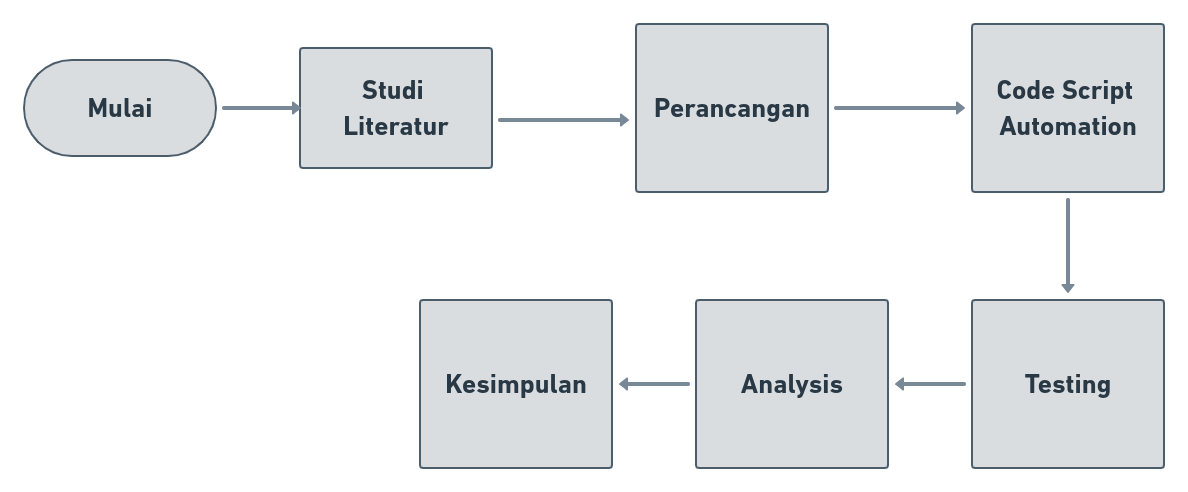
\includegraphics[width=1\textwidth]{figures/Tahapan Skripsi.png}
    \caption{Rancangan Penelitian}
\end{figure}

\section{Studi Literatur}\label{sec:studi_literatur}
Pada tahap studi literatur, peneliti mengumpulkan teori-teori,
konsep, dan temuan penelitian terdahulu yang relevan sebagai landasan dalam melakukan pengembangan dan implementasi automasi deployment menggunakan Argo CD pada lingkungan Kubernetes.
Studi literatur ini dilakukan dengan menelaah berbagai sumber seperti buku, jurnal nasional dan internasional, serta dokumentasi resmi terkait GitOps dan Argo CD.

Peneliti mempelajari konsep dasar GitOps yang menekankan penggunaan repository Git sebagai sumber kebenaran (single source of truth) untuk seluruh konfigurasi dan deployment aplikasi \cite{Weaveworks2017}.
Selain itu, peneliti juga mengkaji dokumentasi resmi Argo CD yang menjelaskan fitur, arsitektur, serta best practice dalam penerapannya pada workflow CI/CD \cite{ArgoCDDocs}.
Penelitian terdahulu dari Korhonen \cite{Korhonen2021} menjadi salah satu referensi utama, di mana dijelaskan penerapan Argo CD untuk meningkatkan konsistensi, efisiensi, dan auditability proses deployment aplikasi pada Kubernetes.

Selain itu, peneliti juga menelaah studi komparatif antara Argo CD dan tools GitOps lain seperti Flux yang dilakukan oleh Sharma et al. \cite{Sharma2022},
serta kajian terkait tantangan keamanan dalam implementasi Argo CD yang dibahas oleh Kumar \cite{Kumar2023}. Dengan mengkaji berbagai referensi tersebut,
peneliti memperoleh pemahaman yang komprehensif mengenai teori dan praktik automasi deployment berbasis GitOps, sehingga dapat merancang dan mengimplementasikan solusi yang sesuai dengan kebutuhan penelitian.

\section{Perancangan (Design)}
Setelah melakukan tahap studi literatur dan analisis kebutuhan sistem, tahap selanjutnya adalah melakukan perancangan sistem automasi deployment yang akan diimplementasikan. Pada tahap studi literatur yang telah dilakukan, peneliti mengambil rancangan dasar dari penelitian-penelitian terdahulu, khususnya model GitOps yang dibahas oleh Ramadoni \cite{Ramadoni2021} dan arsitektur Argo CD yang dijelaskan oleh Korhonen \cite{Korhonen2021}.

Pada tahap ini, peneliti melakukan modifikasi terhadap rancangan yang sudah ada untuk mengadaptasi implementasi Argo CD pada lingkungan bare-metal (non-cloud) dengan memanfaatkan platform virtualisasi Proxmox. Modifikasi ini penting dilakukan karena sebagian besar implementasi GitOps dan Argo CD yang ada di literatur berfokus pada lingkungan cloud \cite{Bolscher2019}, sementara penelitian ini bertujuan untuk mengimplementasikan solusi serupa pada infrastruktur on-premise.
Perancangan yang dilakukan meliputi beberapa aspek utama, yaitu:

\begin{enumerate}
    \item Perancangan arsitektur sistem automasi deployment menggunakan Argo CD pada lingkungan Kubernetes yang berjalan di atas Proxmox
    \item Perancangan alur kerja sistem sesuai dengan pendekatan pull-based deployment yang merupakan karakteristik utama dari GitOps \cite{Weaveworks2017}
    \item Perancangan mekanisme continuous integration yang terintegrasi dengan Argo CD untuk membentuk pipeline CI/CD yang lengkap
    \item Perancangan strategi deployment dan rollback yang efektif untuk aplikasi berbasis microservice
\end{enumerate}

\section{Implementasi Code Automasi (Coding)}
Pada tahap implementasi ini dilakukan penulisan kode terhadap beberapa microservice yang akan menjadi usecase yang akan digunakan menggunakan bahasa Go.
Pada tahap ini juga akan dilakukan automasi script untuk membuat infrastruktur dimana ArgoCD akan berjalan. Tahap implementasi akan menghasilkan sebuah sistem automasi, microservices,
beserta infrastructur tempat berjalannya ArgoCD yaitu infrastructure kubernetes.

\section{Pengujian dan Analisis (Testing dan Analysis)}
Dalam pengujian dan analisis hasil dari implementasi yang dibuat akan dilakukan tahap pengujian terlebih dahulu.
Pengujian dan analisis dilakukan untuk mencari dan mengidentifikasi kesalahan pada sebuah sistem. Pengujian akan dilakukan menggunakan black-box testing dengan metode validasi User Acceptance Testing
dengan kriteria usability testing.

\section{Kesimpulan}
Kesimpulan adalah tahapan terakhir setelah dilakukan implementasi dan pengujian. Pada tahap ini peneliti akan membuat kesimpulan untuk bertujuan
mengetahui letak kelebihan dan kekurangan sistem yang telah dikembangkan.
\newpage


\onehalfspacing
\renewcommand{\chaptername}{BAB}
%-----------------------------------------------------------------------------%
\chapter{HASIL DAN PEMBAHASAN}
%-----------------------------------------------------------------------------%
\vspace{4.5pt}
\setlength{\parskip}{0.5em}
\section{Perancangan (Design)}\label{sec:bab4_perancangan}
Pada tahan pertama ini peneliti akan melakukan perancangan sebuah infrastruktur dimana sistem Kubernetes dan ArgoCD akan dijalankan lalu
microservice untuk dilakukan simulasi implementasi pada ArgoCD. Semua rancangan akan menggunakan visualisasi diagram secara garis besar (high-level) agar mudah dipahami.

\subsection{Sistem Arsitektur Infrastruktur}
Peneliti menggunakan Proxmox VE (Virtual Environment) yang didalam nya terdapat Virtual Machine berupa Talos OS Linux yang siap digunakan untuk menjalankan Kubernetes cluster
\begin{figure}[H]
    \centering
    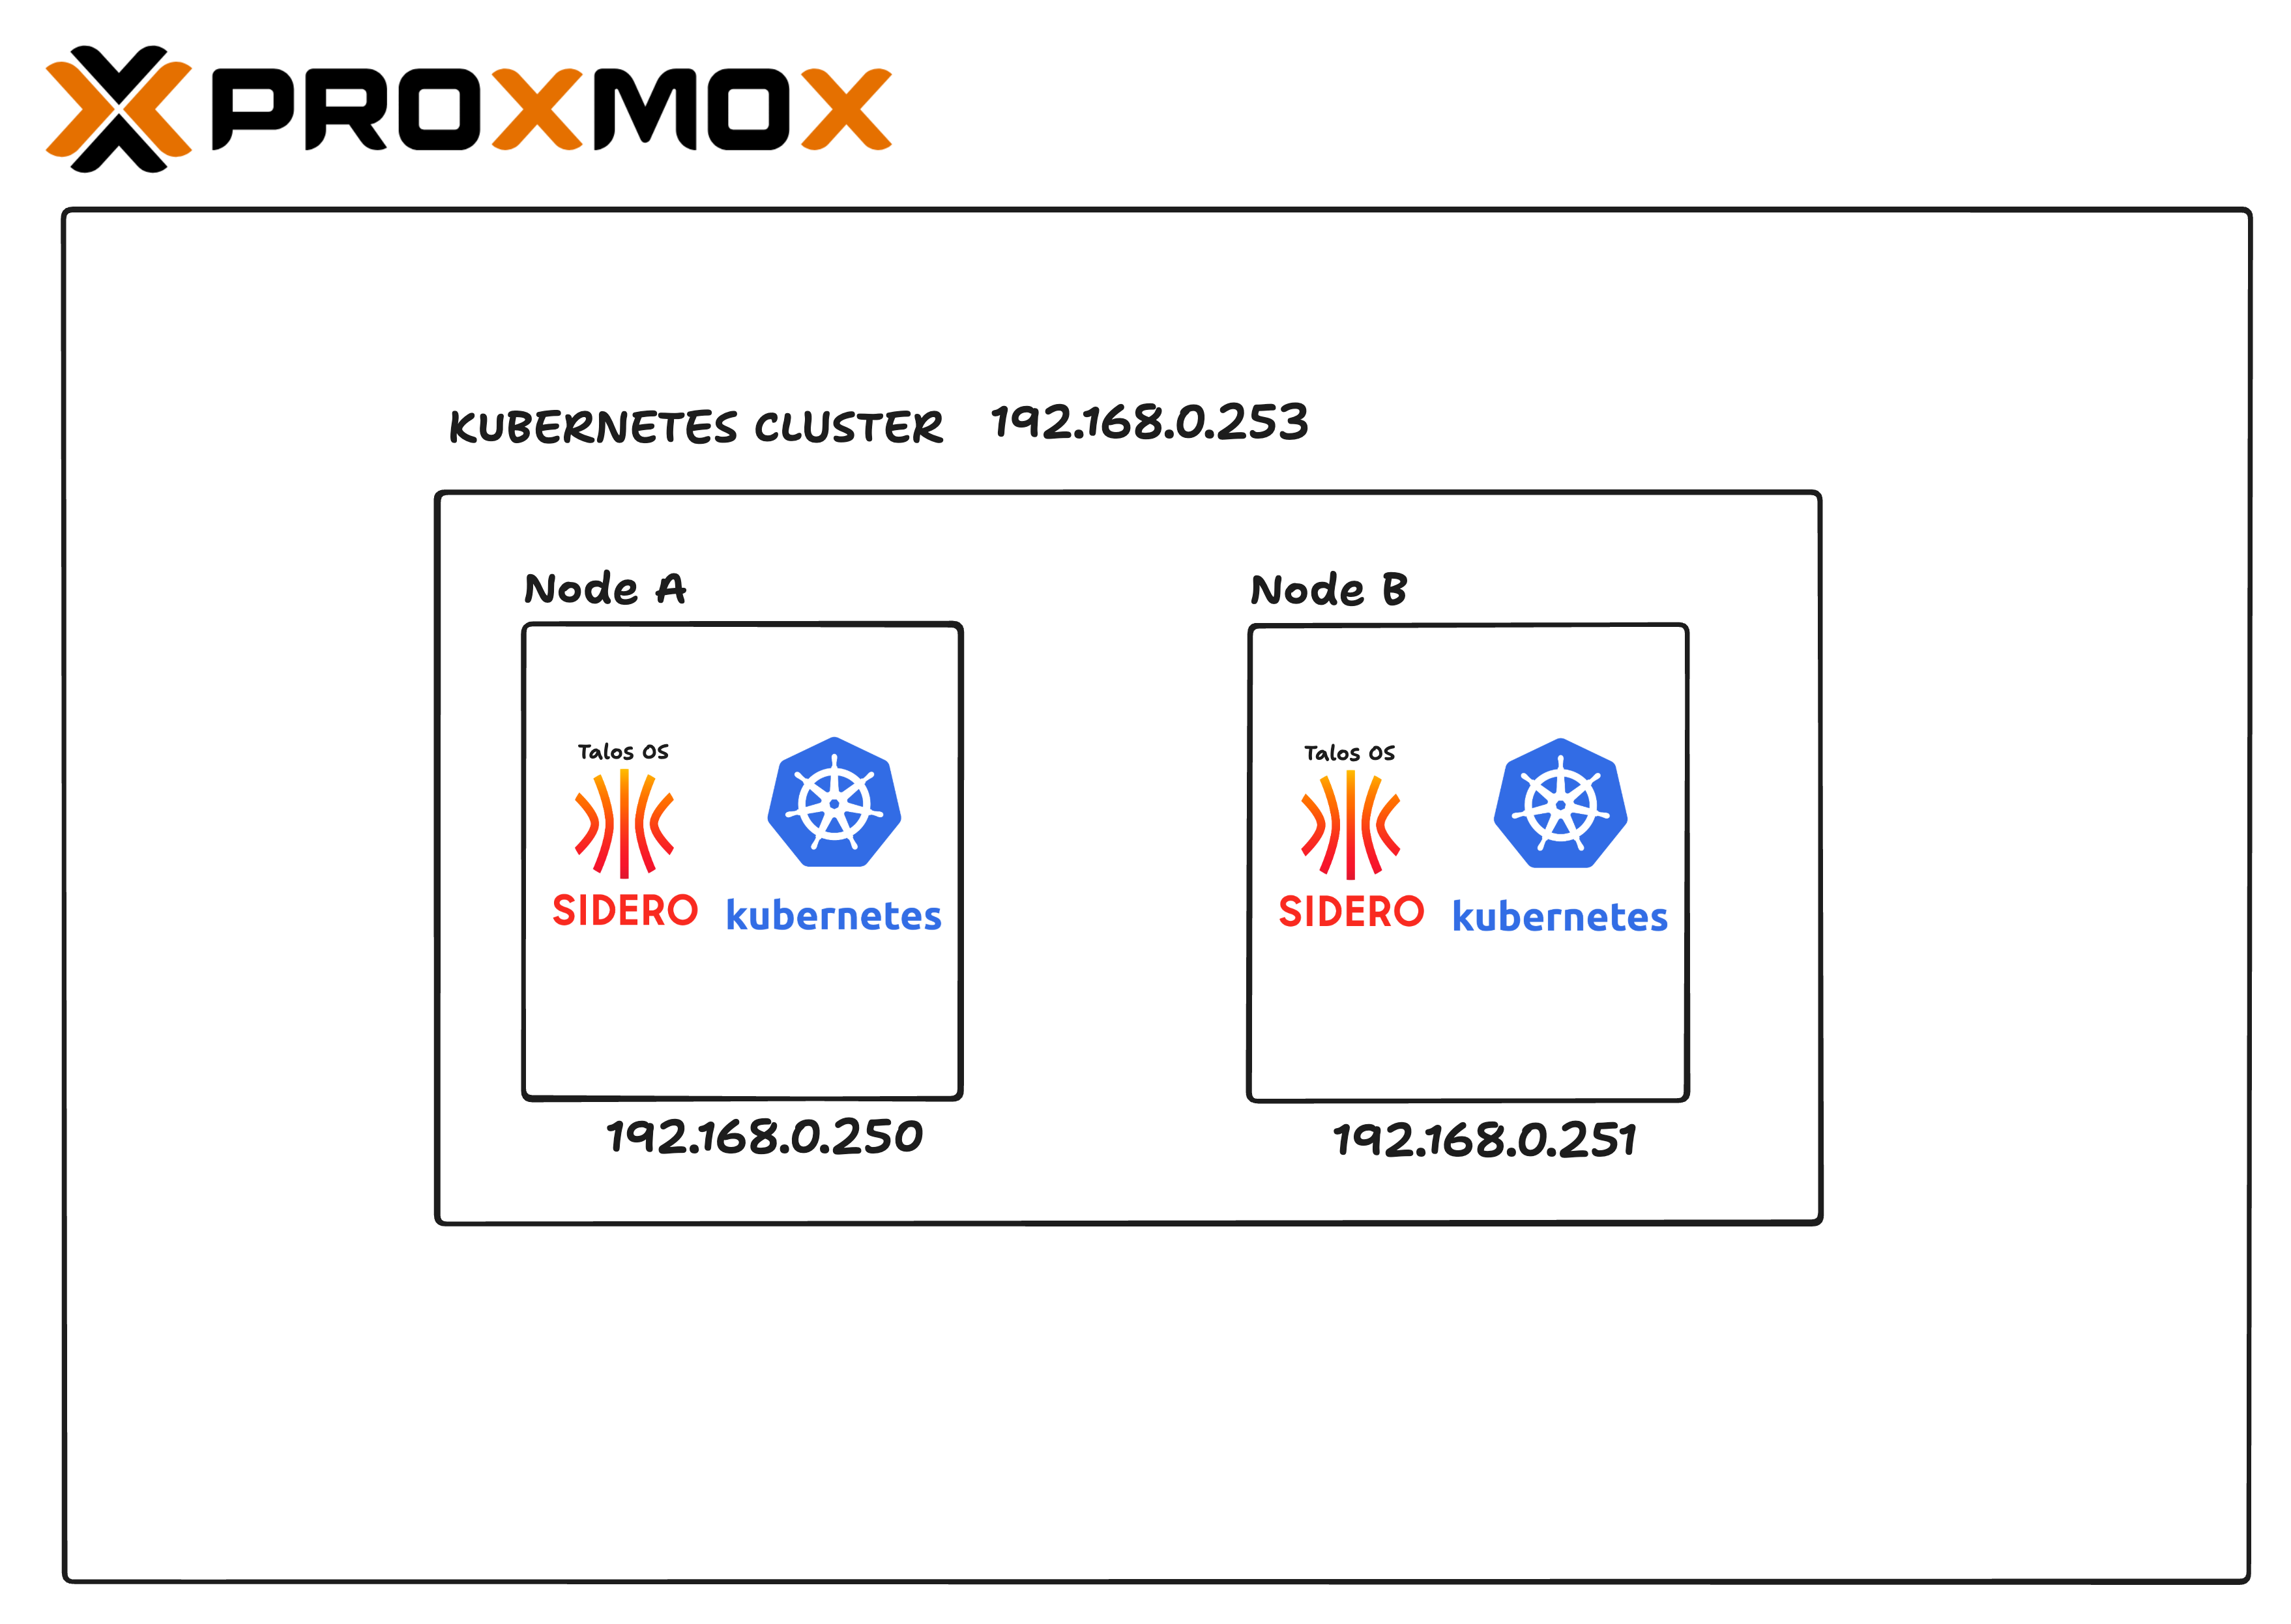
\includegraphics[width=0.9\textwidth]{figures/proxmox-cluster.png}
    \caption{Arsitektur Infrastruktur High Level}
    \label{fig:arsitektur_infrastruktur}
\end{figure}

\subsection{Sistem Arsitektur Kubernetes Cluster}
Pada bagian sebelumnya peneliti sudah memaparkan arsitektur infrastruktur dimana Kubernetes cluster akan berjalan. Pada tahap ini peneliti akan
memaparkan arsitektur pada Kubernetes cluster nya itu sendiri dimana ArgoCD akan berjalan.

\begin{figure}[H]
    \centering
    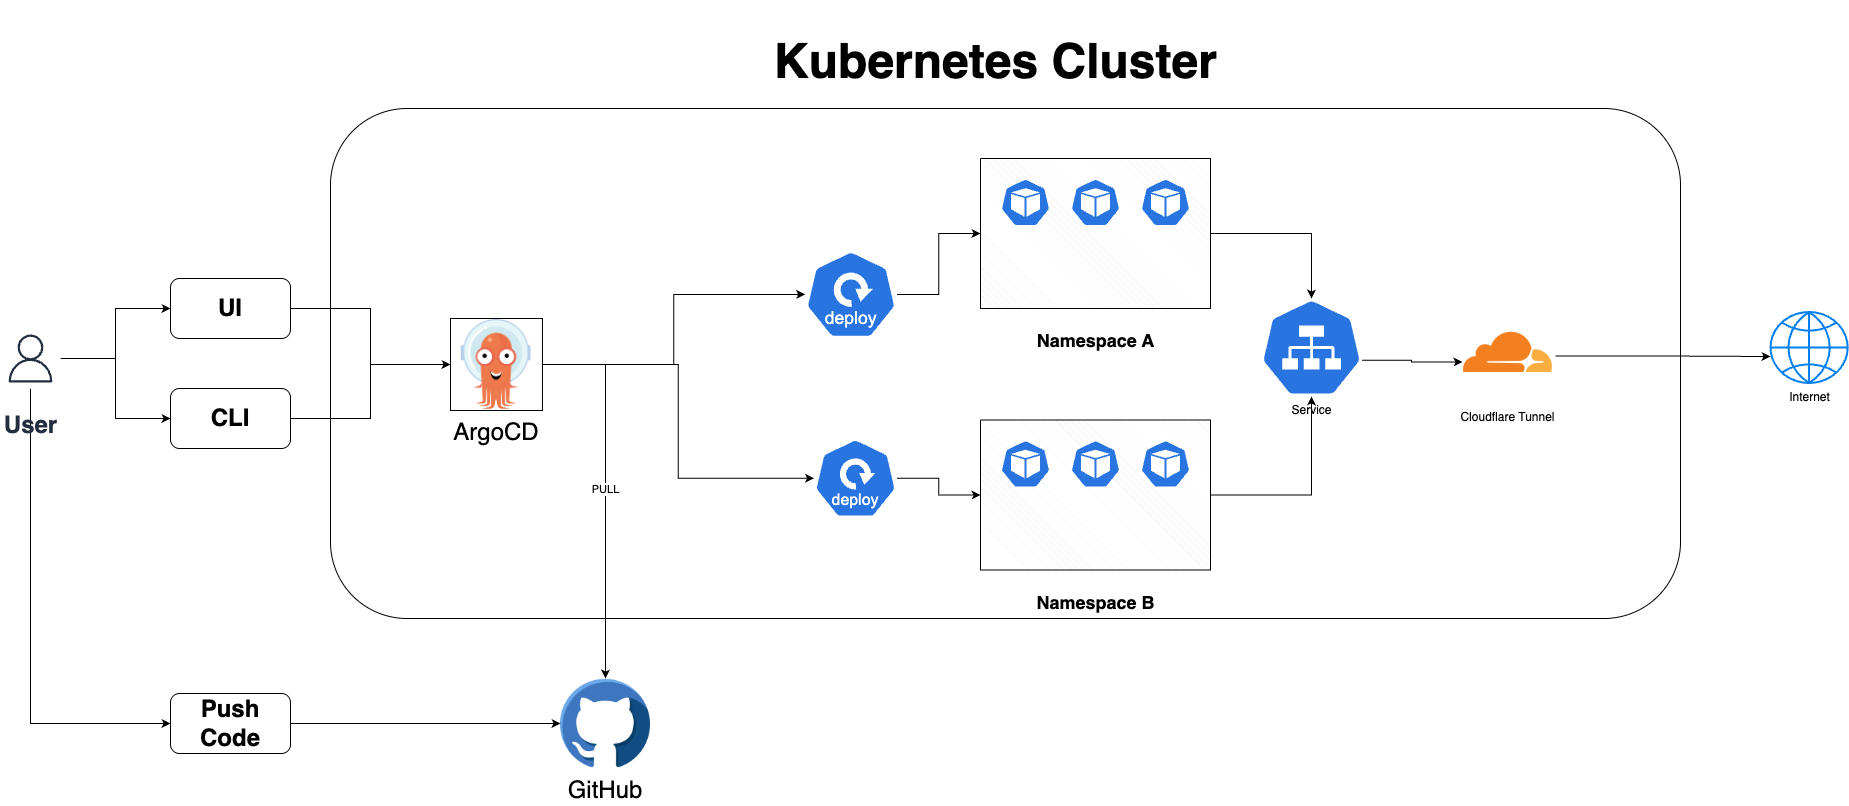
\includegraphics[width=0.9\textwidth]{figures/kube-new.png}
    \caption{Arsitektur Kubernetes High Level}
    \label{fig:arsitektur_kubernetes}
\end{figure}

Didalam sistem Kubernetes cluster yang dibuat terdapat komponen ArgoCD dan Cloudflare Tunnel (optional) yang bertujuan agar server
microservice bisa diakses pada world wide web (internet).

\section{Pengkodean (Coding) / Implementasi}
Tahap ini peneliti akan menjabarkan secara rinci pengkodean/implementasi rancangan sistem yang sudah dirancang.
Peneliti akan melakukan implementasi rancangan sistem menggunakan beberapa komponen yaitu
\begin{enumerate}
    \item Proxmox VE (versi 8.4)
    \item Talos OS (versi 1.9.5)
    \item Kubernetes
    \item ArgoCD
    \item Cloudflare Tunnel
    \item Git repository (GitHub)
\end{enumerate}

\subsection{Implementasi Proxmox VE}
Untuk implementasi Proxmox VE sendiri peneliti melakukan instalasi proxmox pada 2 mesin dengan arsitektur CPU X86.
Pertama kita akan download ISO file atau installer proxmox yang terdapat di link ini \verb|https://enterprise.proxmox.com/iso/proxmox-ve_8.4-1.iso|.
Setelah itu kita memerlukan sebuah Flashdisk atau media untuk bootable ISO tersebut disini peneliti menggunakan tools yang bernama Rufus

\begin{figure}[H]
    \centering
    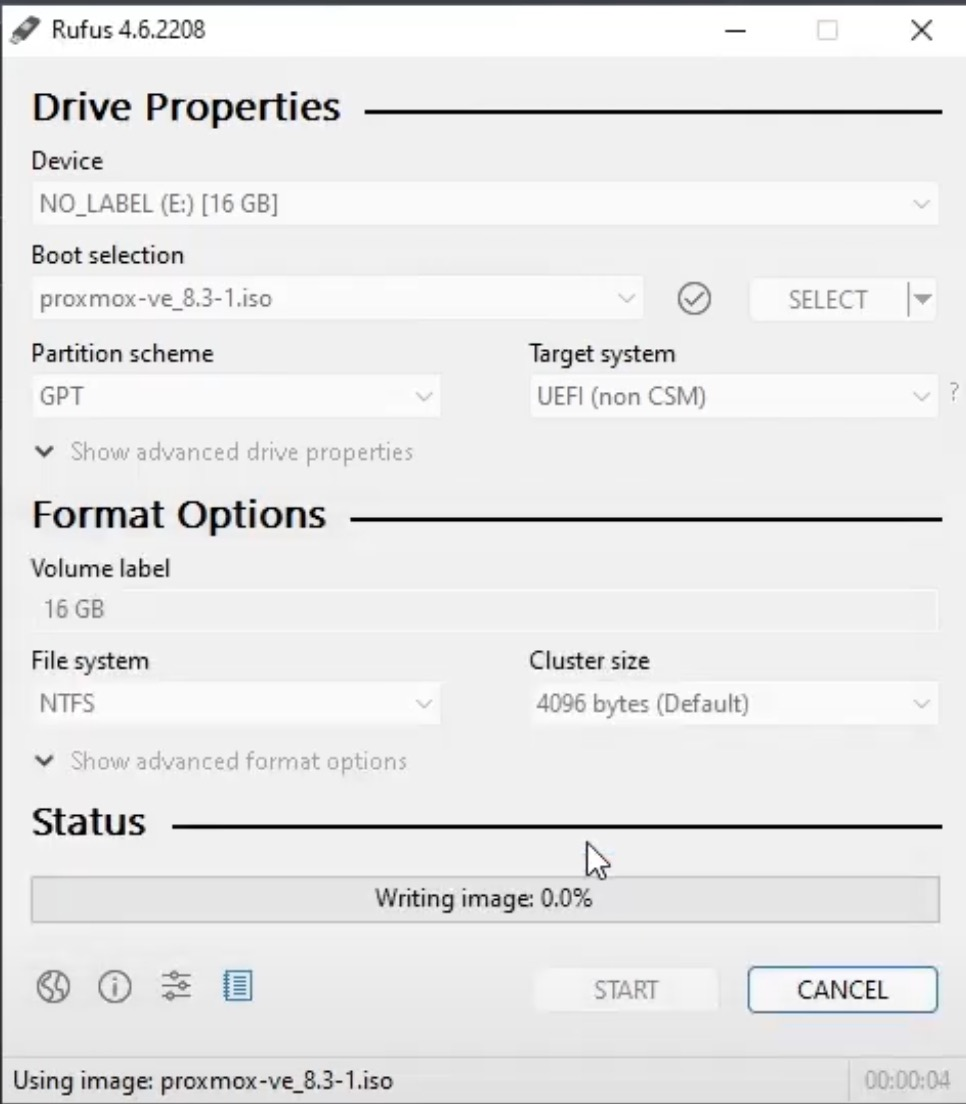
\includegraphics[width=0.8\textwidth]{figures/proxmox-install-rufus-1.jpg}
    \caption{Proses Pembuatan Bootable Proxmox Menggunakan Rufus}
    \label{fig:proxmox_rufus}
\end{figure}

Setelah itu kita perlu mengganti bootable menu yang mengarah pada flashdisk atau media yang kita gunakan untuk instalasi proxmox ketika booting BIOS pada mesin yang digunakan.
Akan terdapat layar instalasi Rufus seperti ini yang akan muncul pada mesin yang kita gunakan.

\begin{figure}[H]
    \centering
    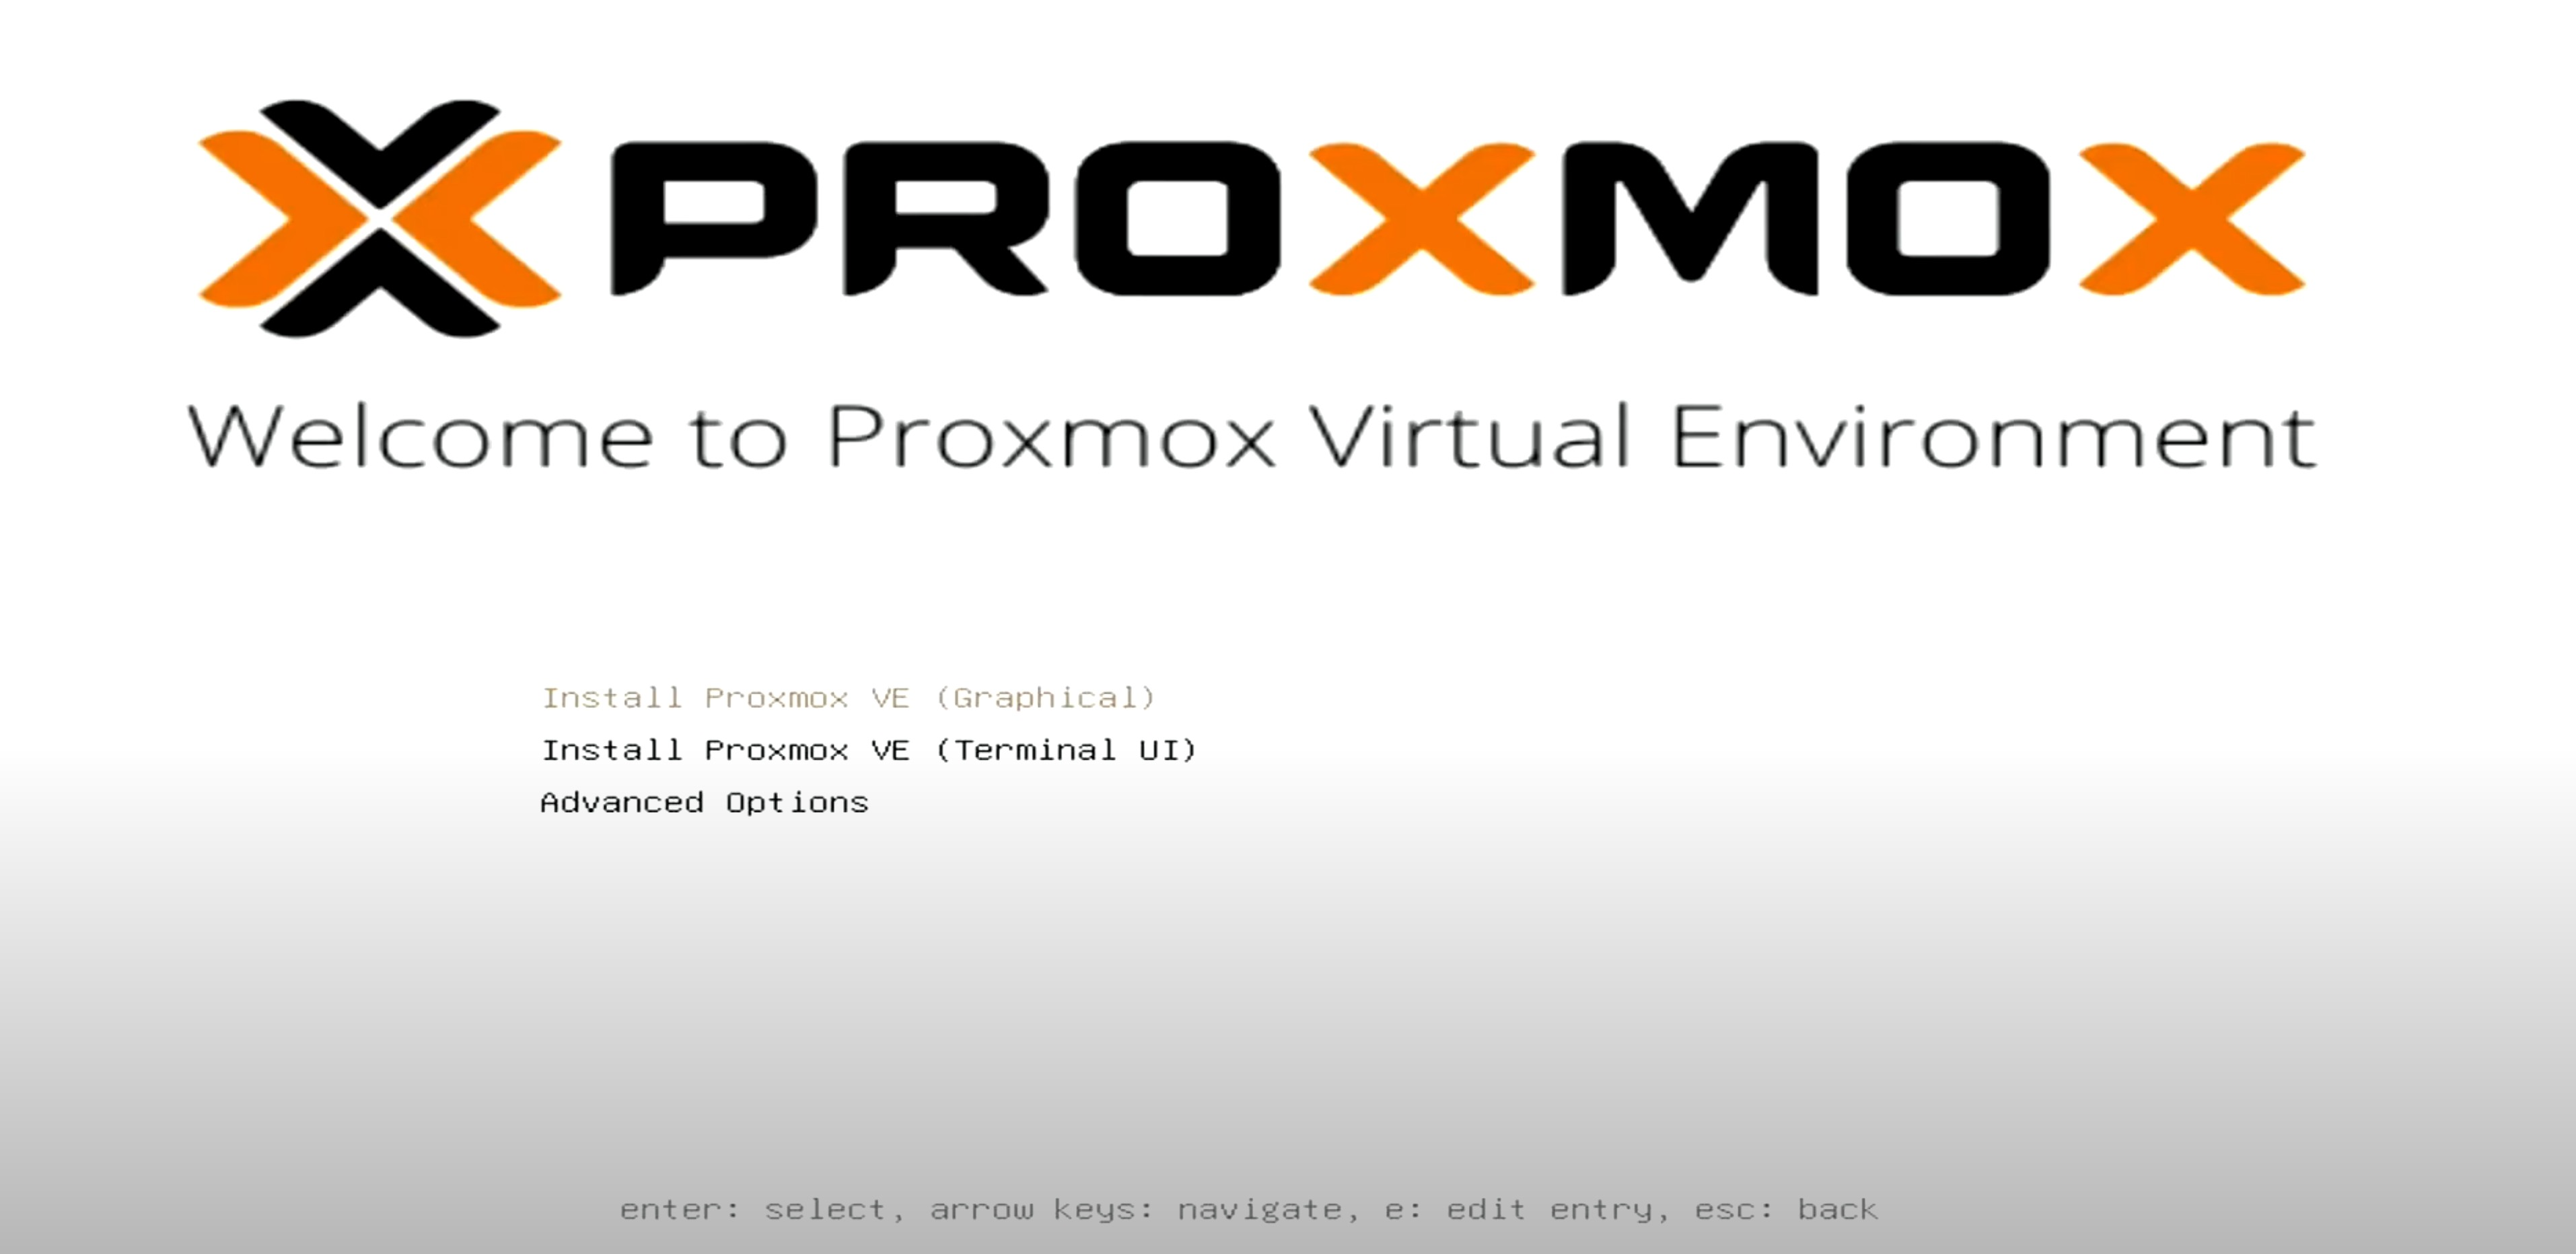
\includegraphics[width=0.8\textwidth]{figures/proxmox-install-ui-2.jpg}
    \caption{Tampilan Awal Instalasi Proxmox VE}
    \label{fig:proxmox_install_ui}
\end{figure}

Selanjutnya kita tinggal mengikuti apa yang diarahkan secara default oleh user interface yang ditampilkan hingga mesin akan restart dan berada pada tampilan seperti ini.
Pada tampilan layar tersebut terdapat server yang bisa kita gunakan untuk akses user interface melalui browser
\begin{figure}[H]
    \centering
    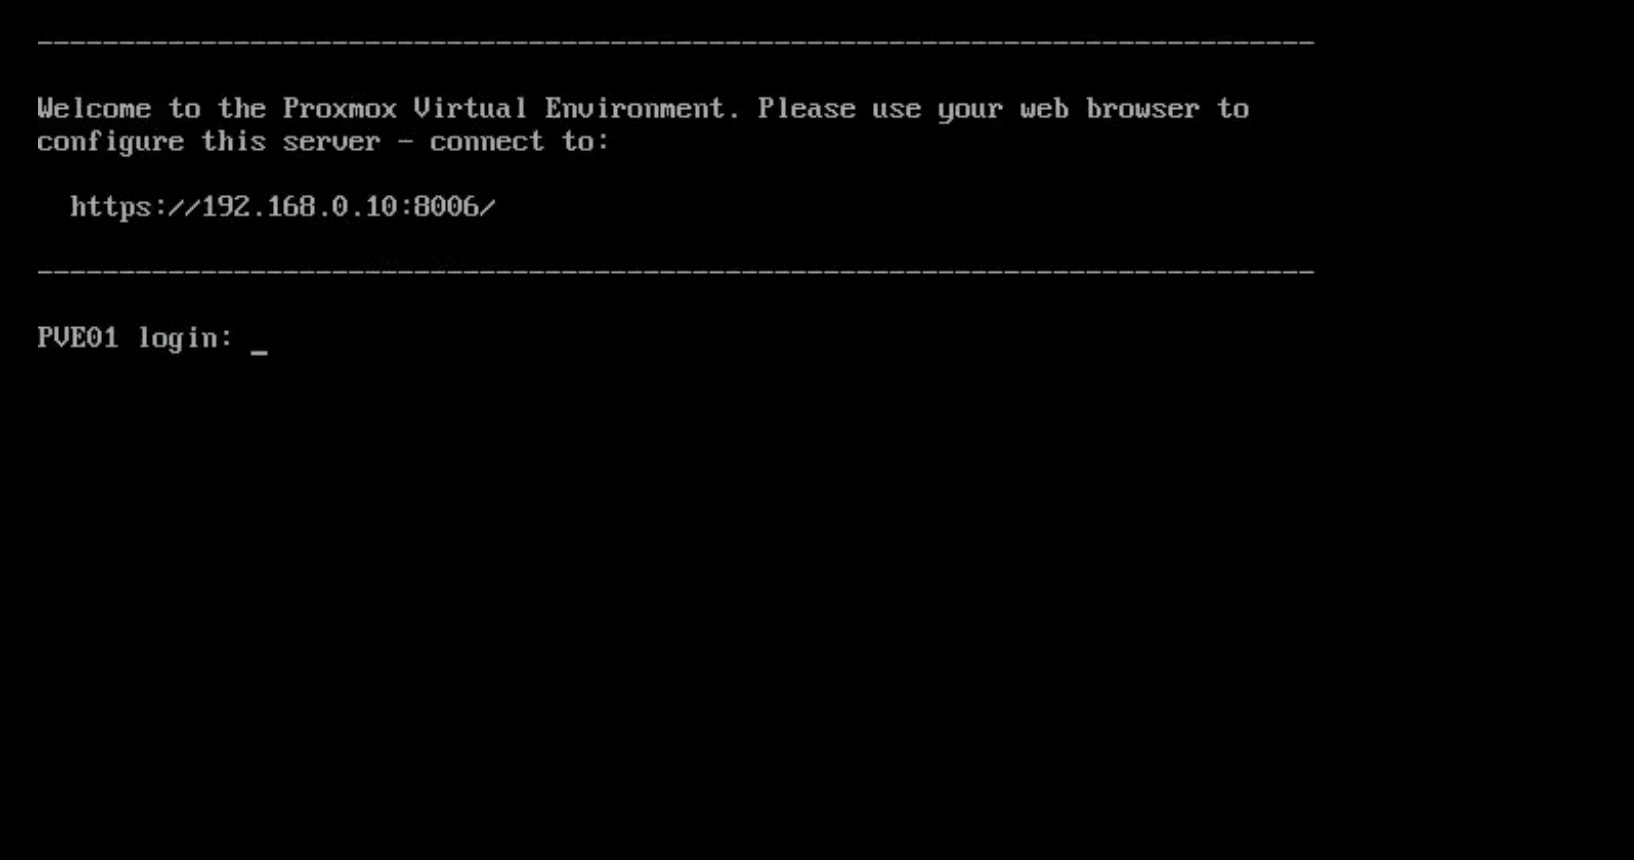
\includegraphics[width=0.8\textwidth]{figures/proxmox-install-terminal-3.jpg}
    \caption{Tampilan Terminal Setelah Instalasi Proxmox Selesai}
    \label{fig:proxmox_terminal}
\end{figure}

Akses UI pada komputer yang ada pada network yang sama dengan Proxmox melalui web user interface.
Peneliti akan mengulang implementasi ini untuk mesin kedua.
\begin{figure}[H]
    \centering
    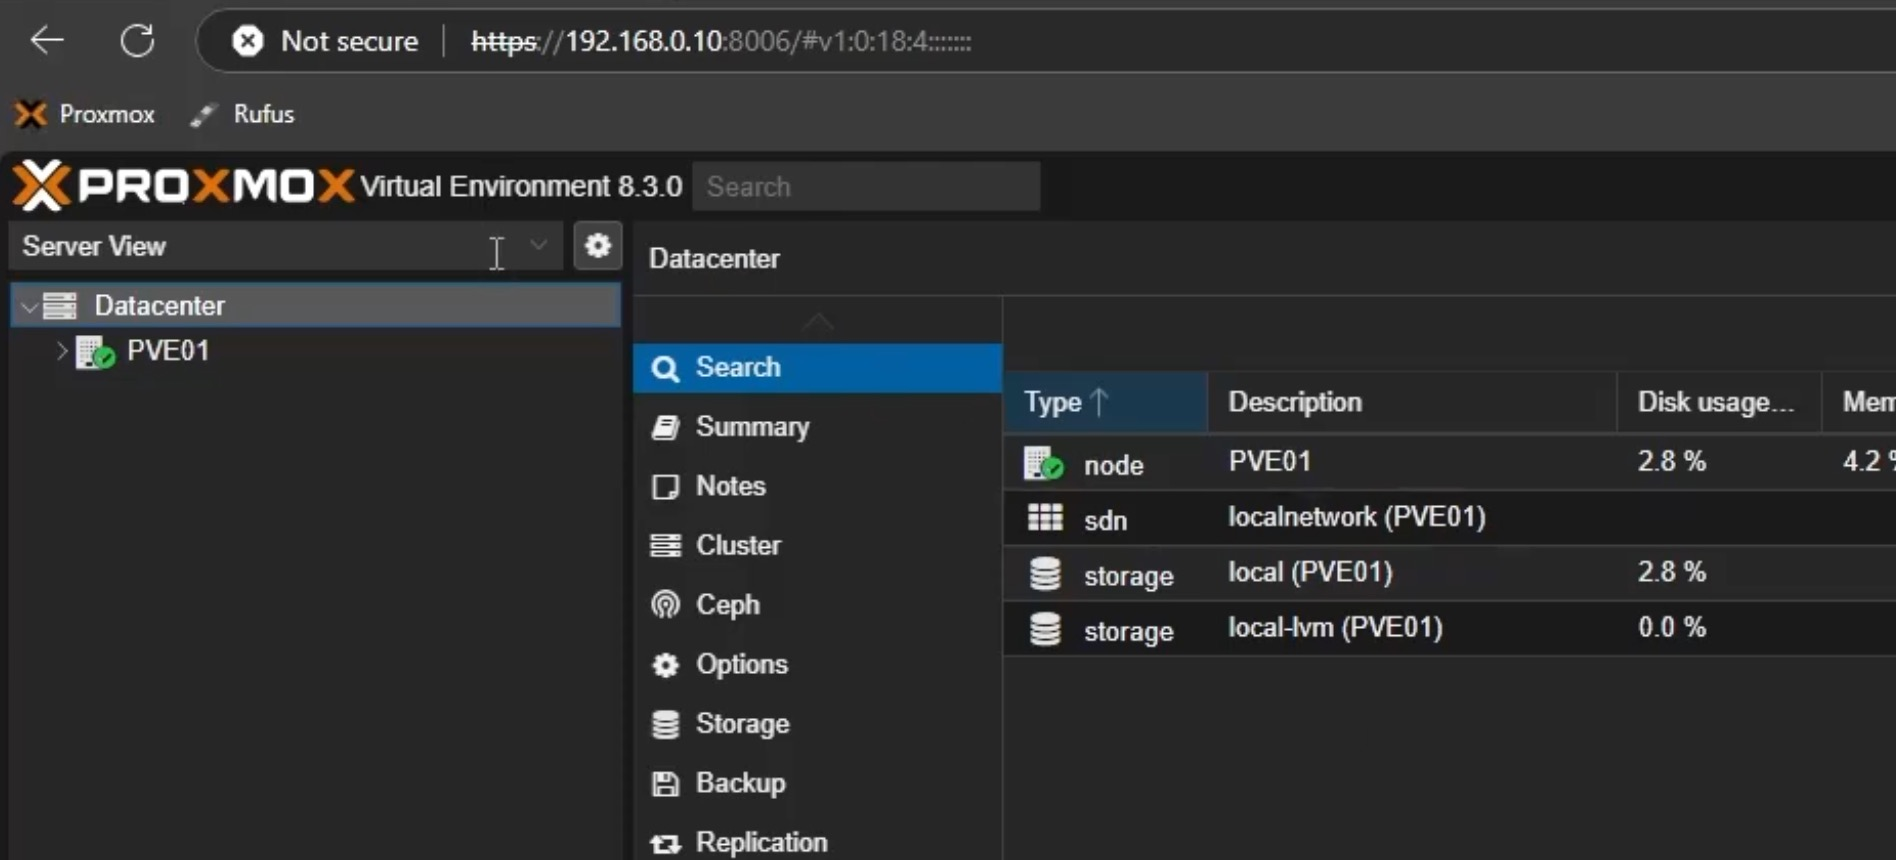
\includegraphics[width=0.9\textwidth]{figures/proxmox-install-web-ui-4.jpg}
    \caption{Tampilan Web Interface Proxmox VE}
    \label{fig:proxmox_webui}
\end{figure}

\subsection{Implementasi Talos OS}
Pada tahap selanjutnya akan dilakukan instalasi Talos OS yang akan di-install menggunakan VM yang ada pada Proxmox VE.
Pertama yang dilakukan adalah mengunduh ISO file Talos OS di sini.

\url{https://github.com/siderolabs/talos/releases/download/v1.9.5/metal-amd64.iso}

\begin{figure}[H]
    \centering
    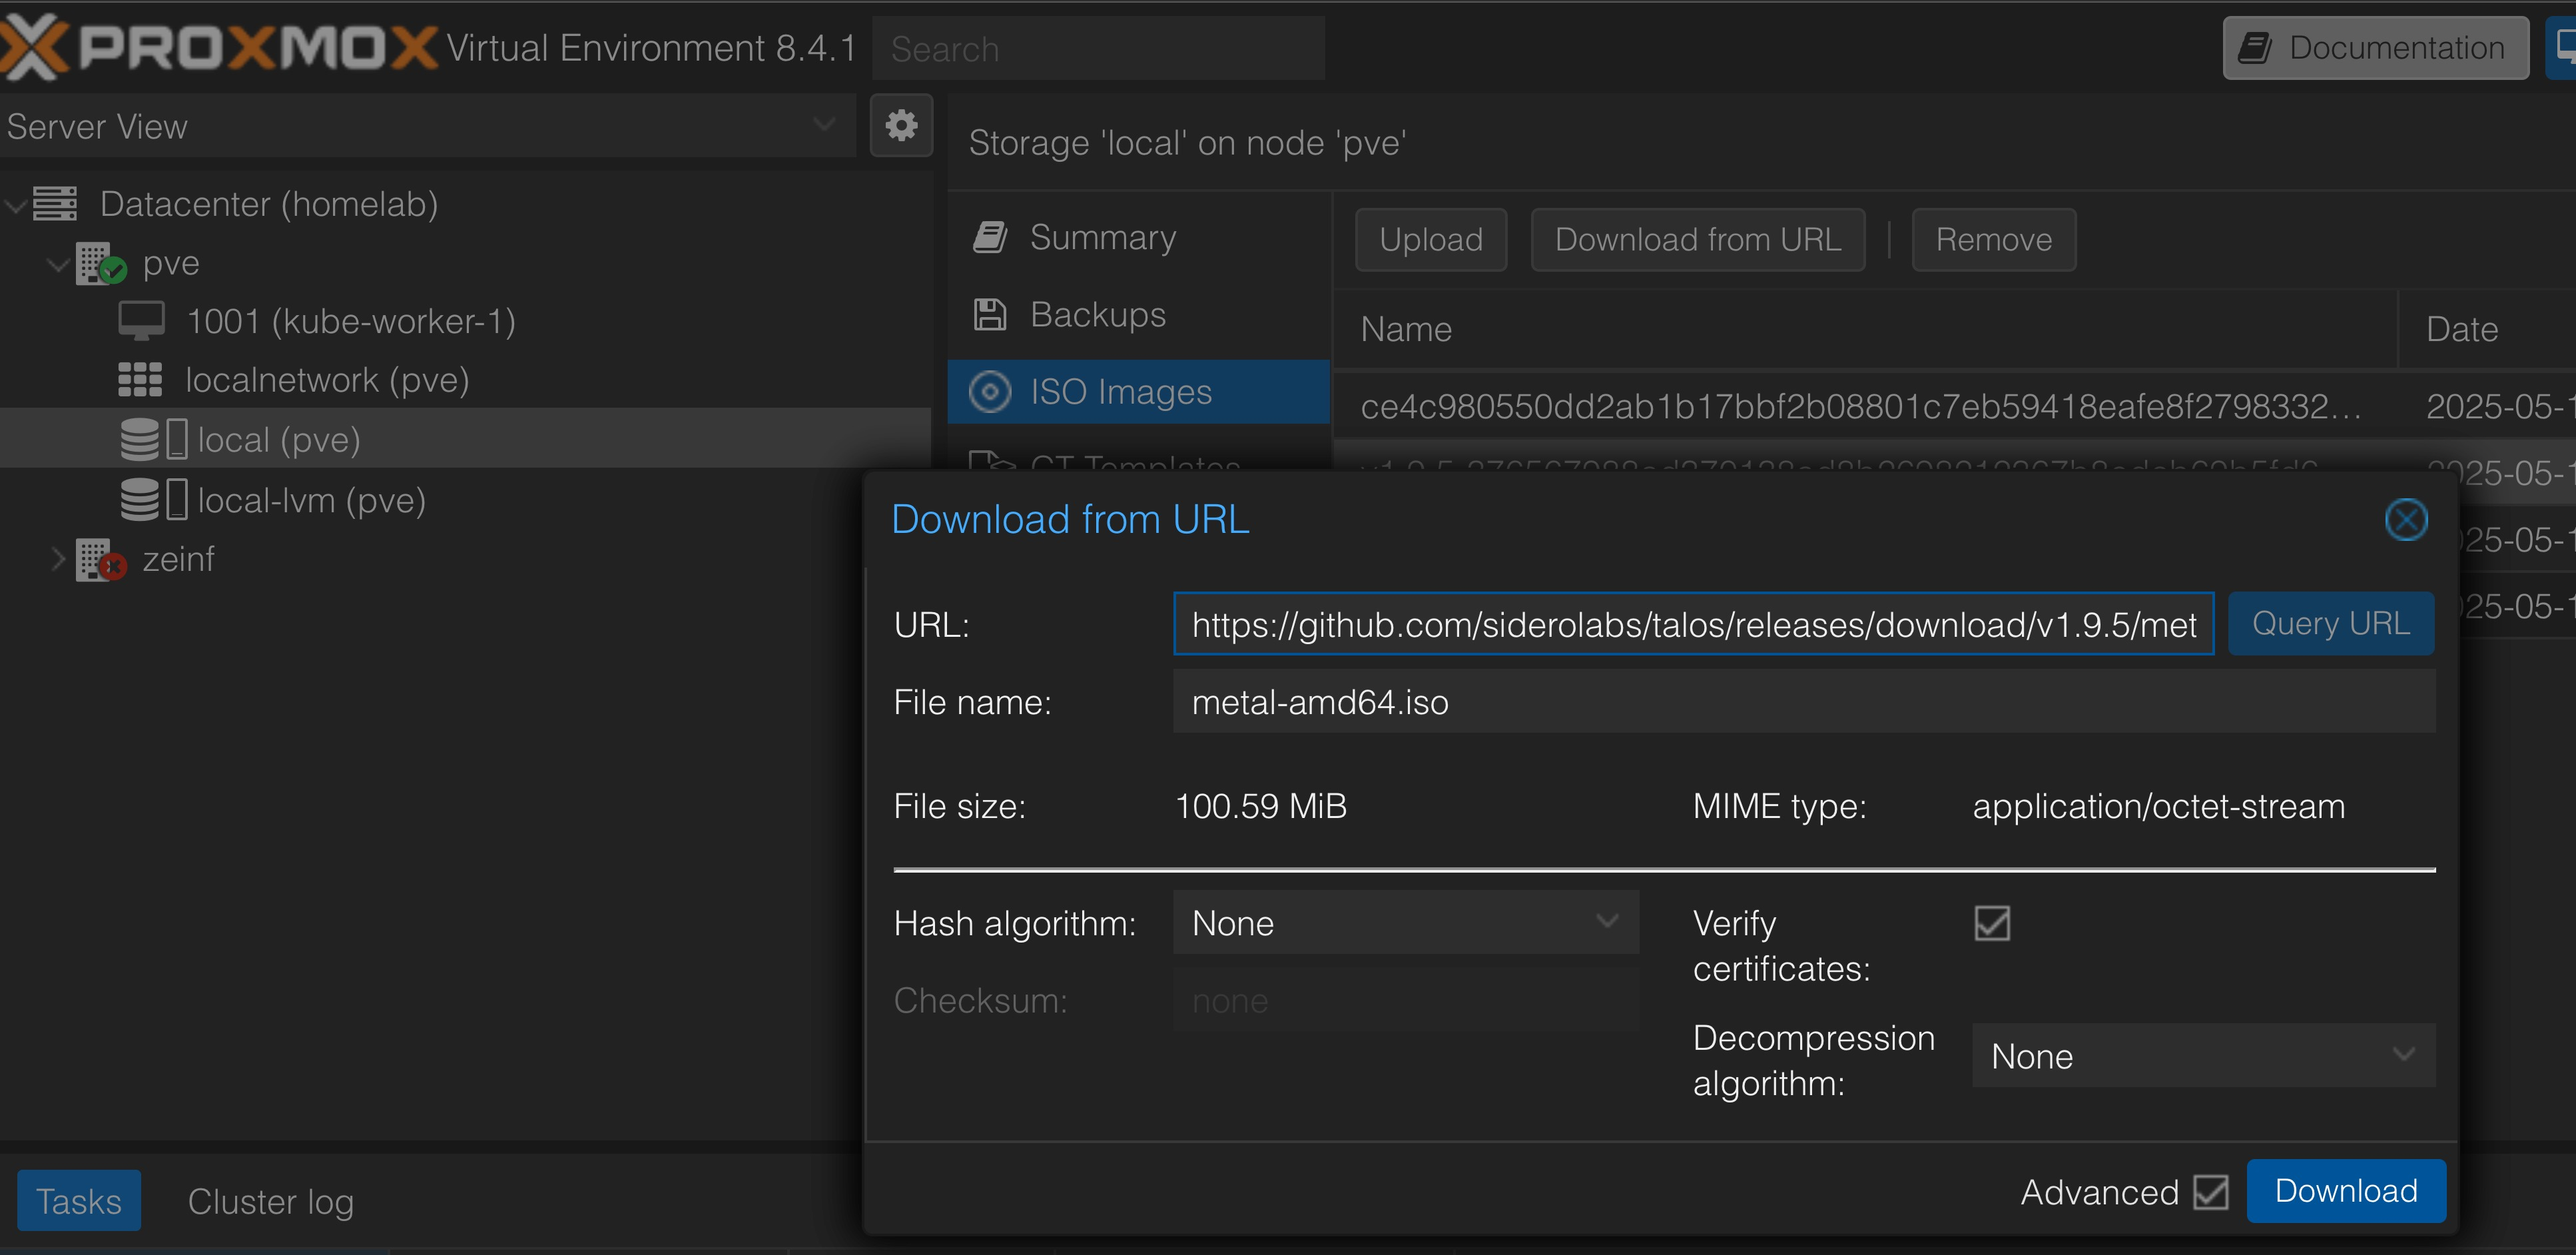
\includegraphics[width=0.8\textwidth]{figures/talos-install-1.jpg}
    \caption{Proses Download ISO Talos OS}
    \label{fig:talos_download}
\end{figure}

Url tersebut lalu didownload melalui proxmox agar tersimpan didalam proxmox. Lalu tahap selanjutnya adalah melakukan instalasi VM Talos OS pada proxmox.

\subsubsection{Instalasi Talos OS}
Tahap ini adalah bagian instalasi VM Talos OS. Peneliti melakukan instalasi pada proxmox VE melalui interface web.
Tahap ini akan dilakukan pada 2 mesin berbeda pada proxmox.

\begin{figure}[!htbp]
    1. Klik Create VM lalu isikan VM ID dan Name untuk VM Talos OS
    \centering
    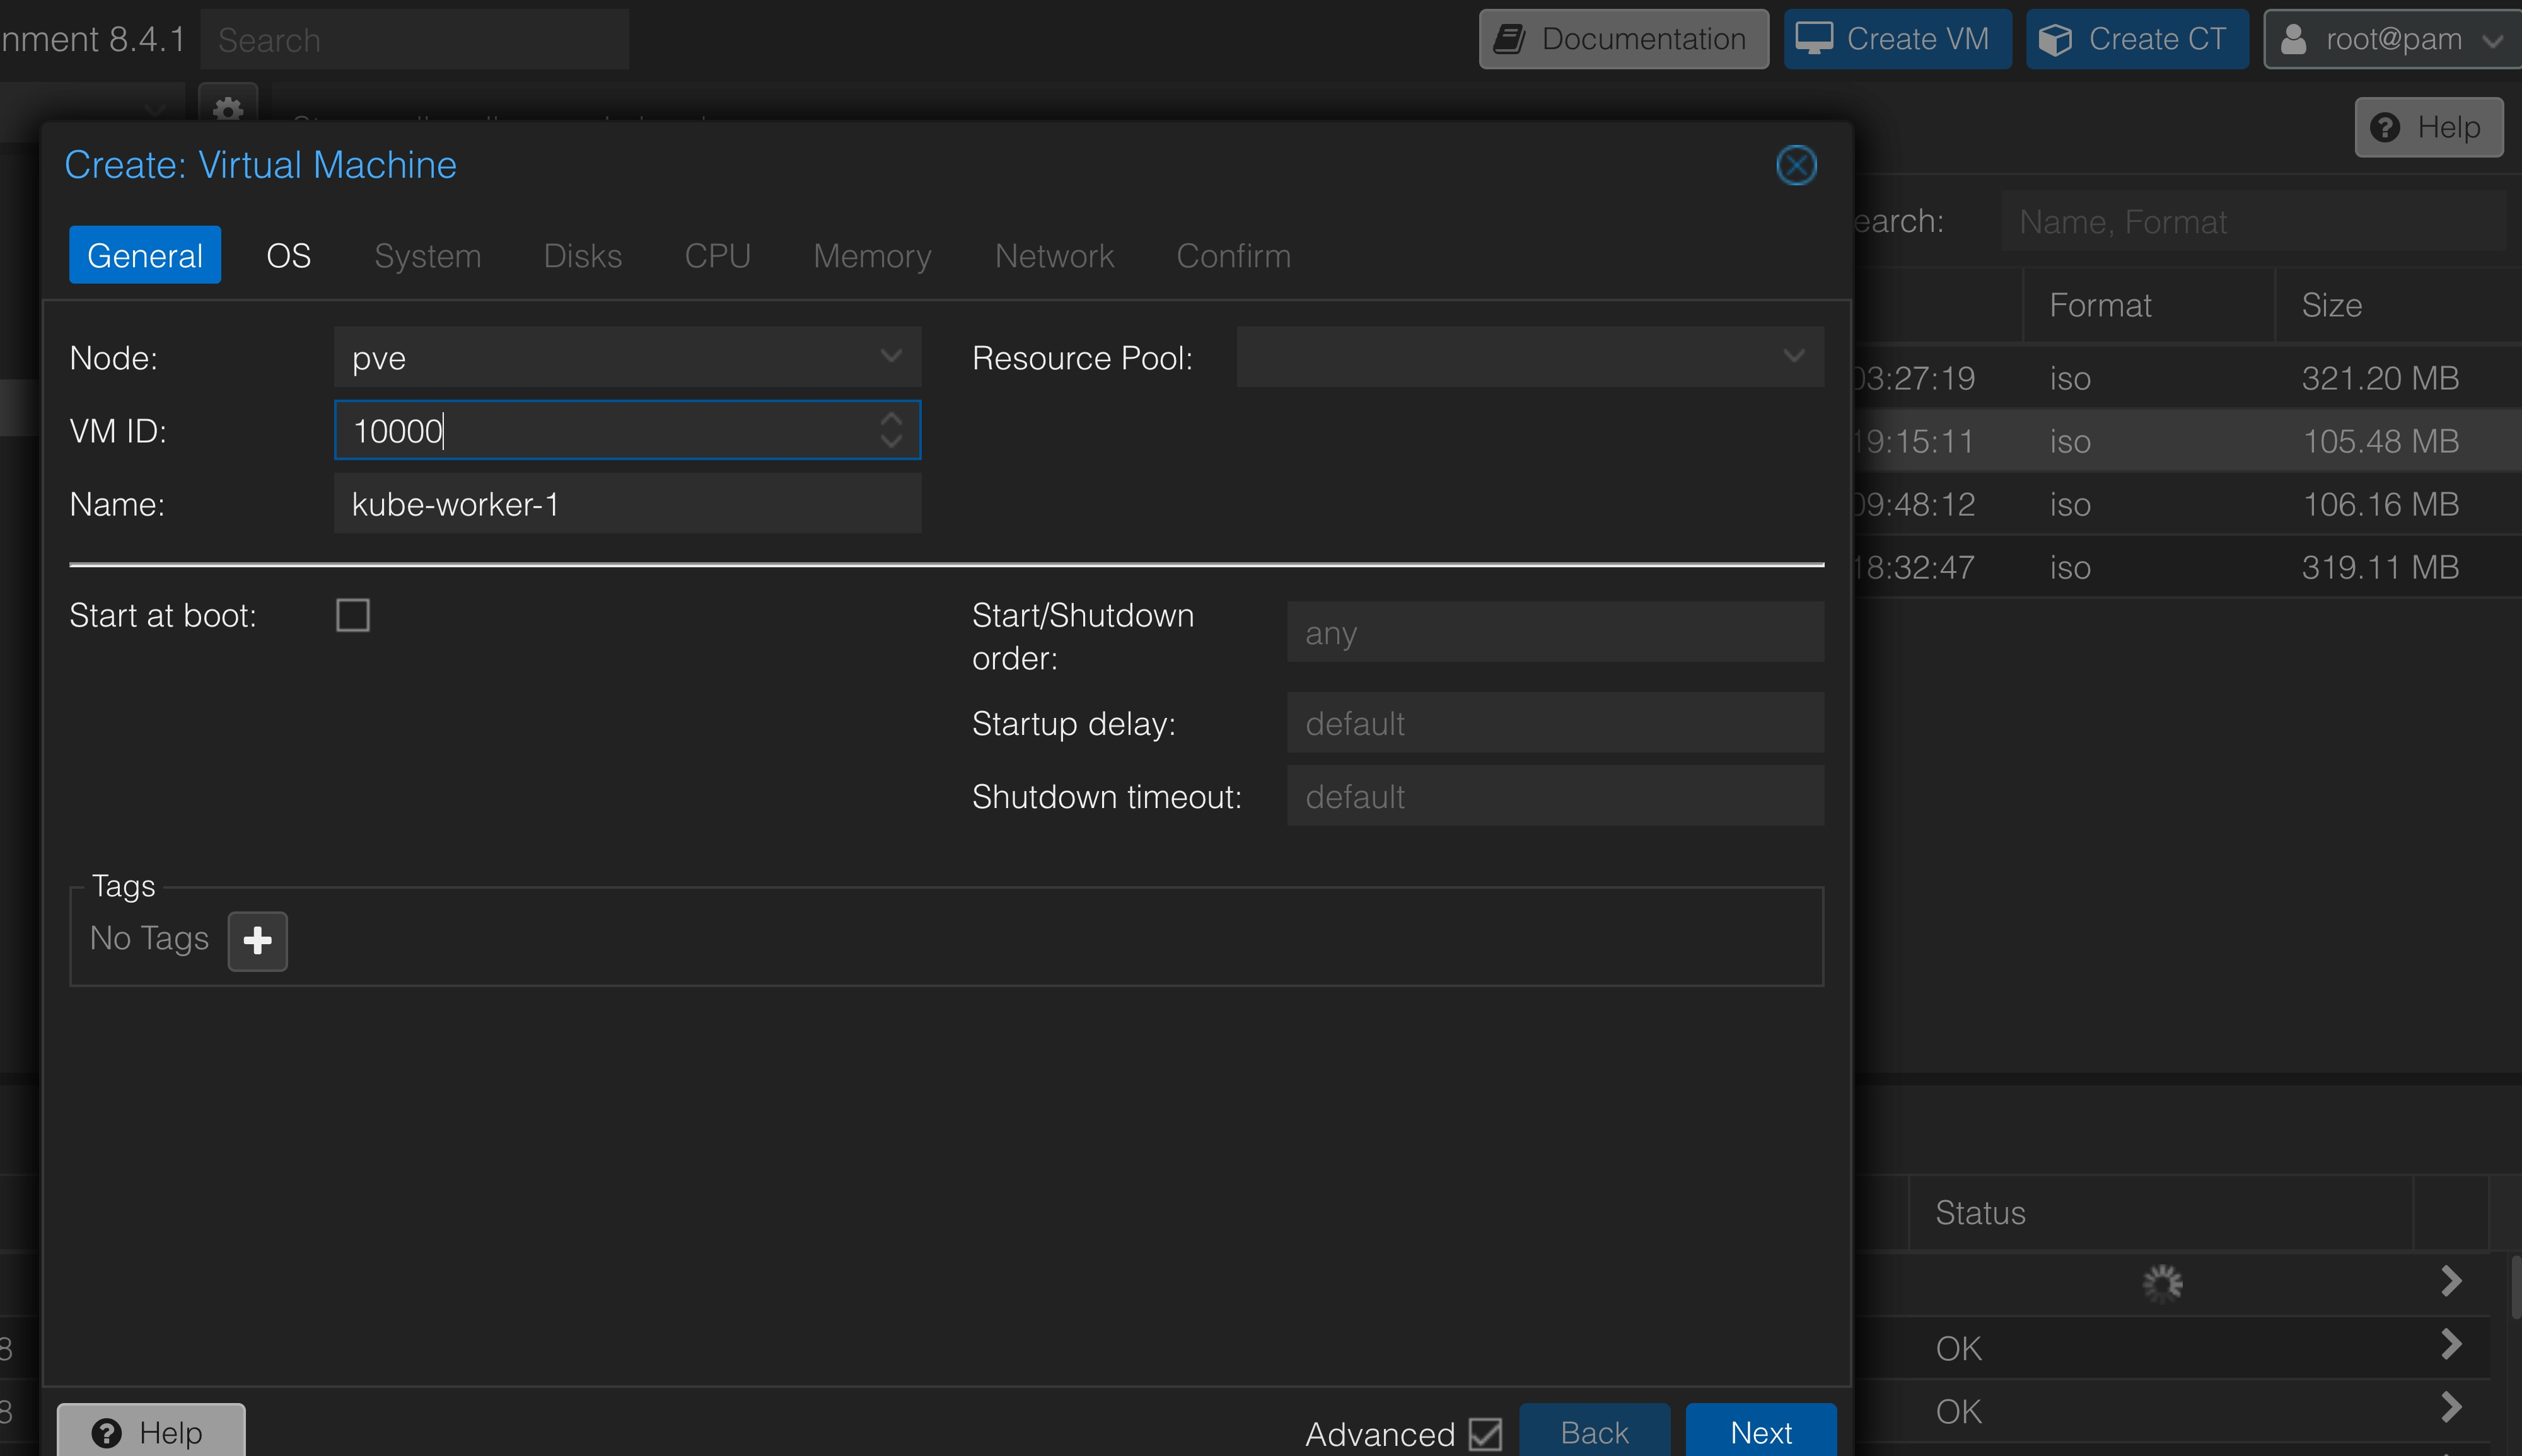
\includegraphics[width=1\textwidth]{figures/talos-install-2.jpg}
    \caption{Instalasi Talos OS 1}
\end{figure}
\begin{figure}[!htbp]
    2. Pada bagian OS. Pilih ISO Talos OS yang baru saja diunduh sebelum nya
    \centering
    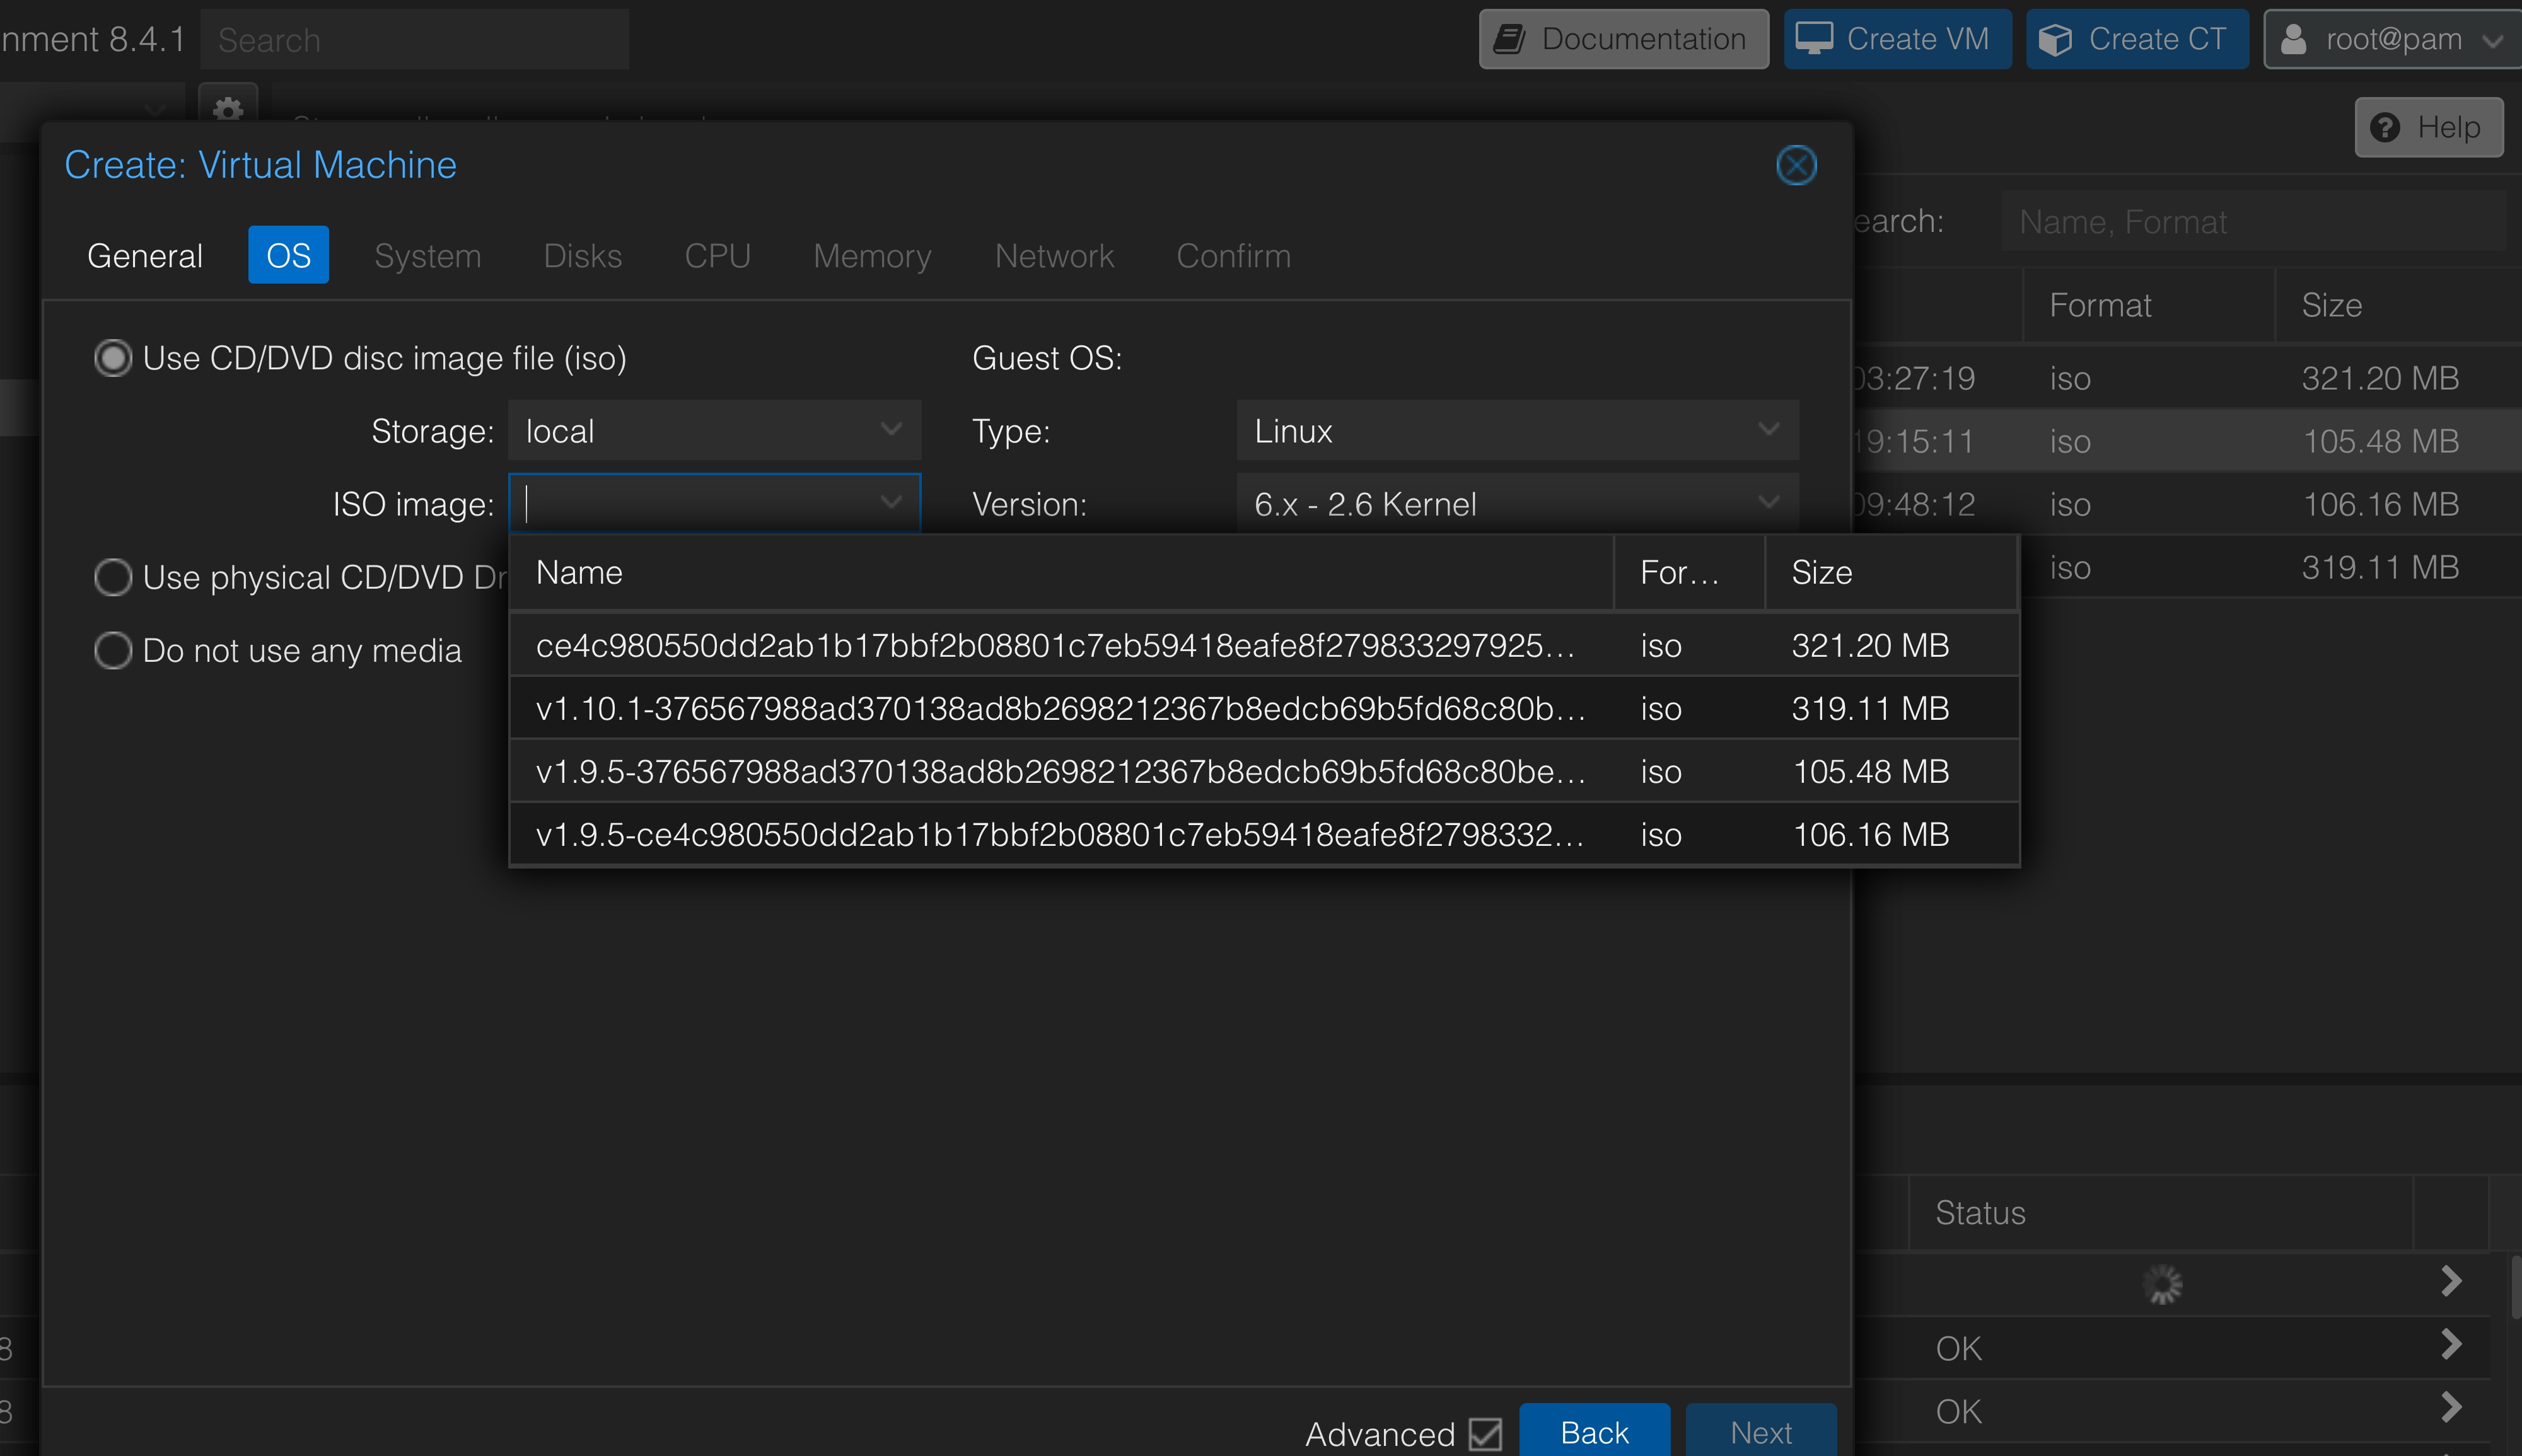
\includegraphics[width=1\textwidth]{figures/talos-install-3.jpg}
    \caption{Instalasi Talos OS 2}
\end{figure}
\begin{figure}[!htbp]
    3. Pada bagian System. cukup next
    \centering
    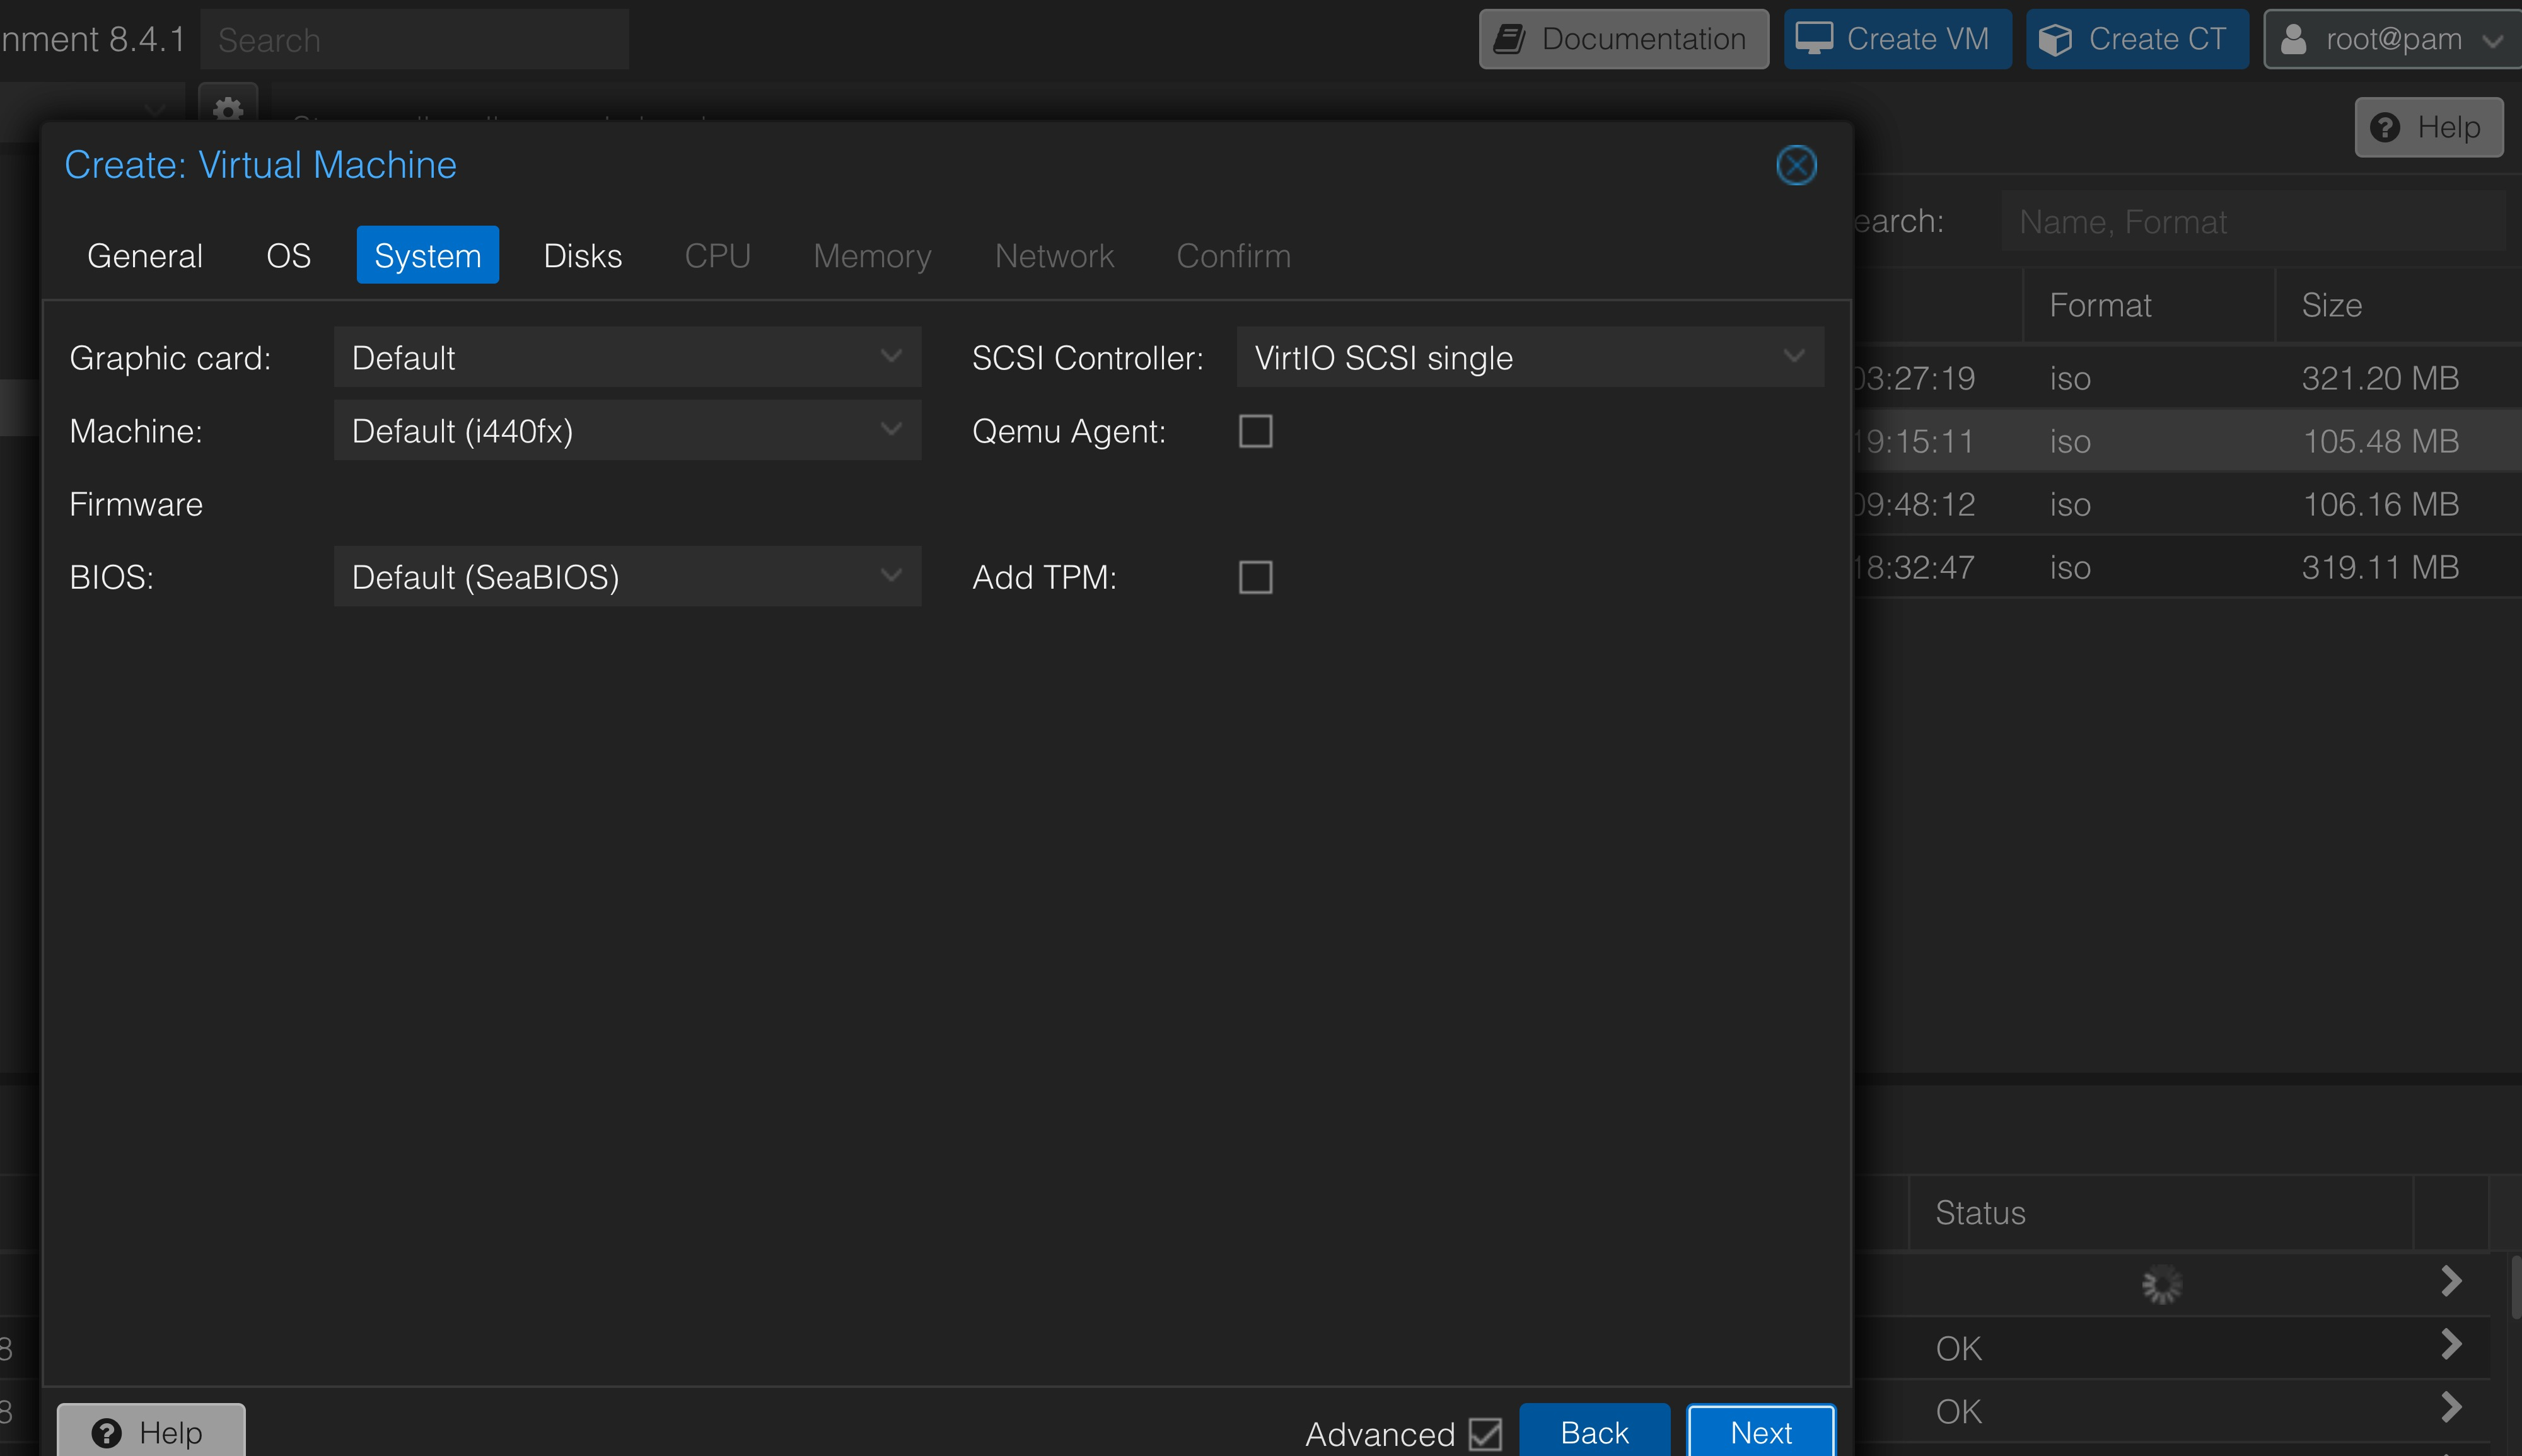
\includegraphics[width=1\textwidth]{figures/talos-install-4.jpg}
    \caption{Instalasi Talos OS 3}
\end{figure}
\begin{figure}[!htbp]
    4. Pada bagian Disk. Cuku merubah bagian Disk size menjadi 100
    \centering
    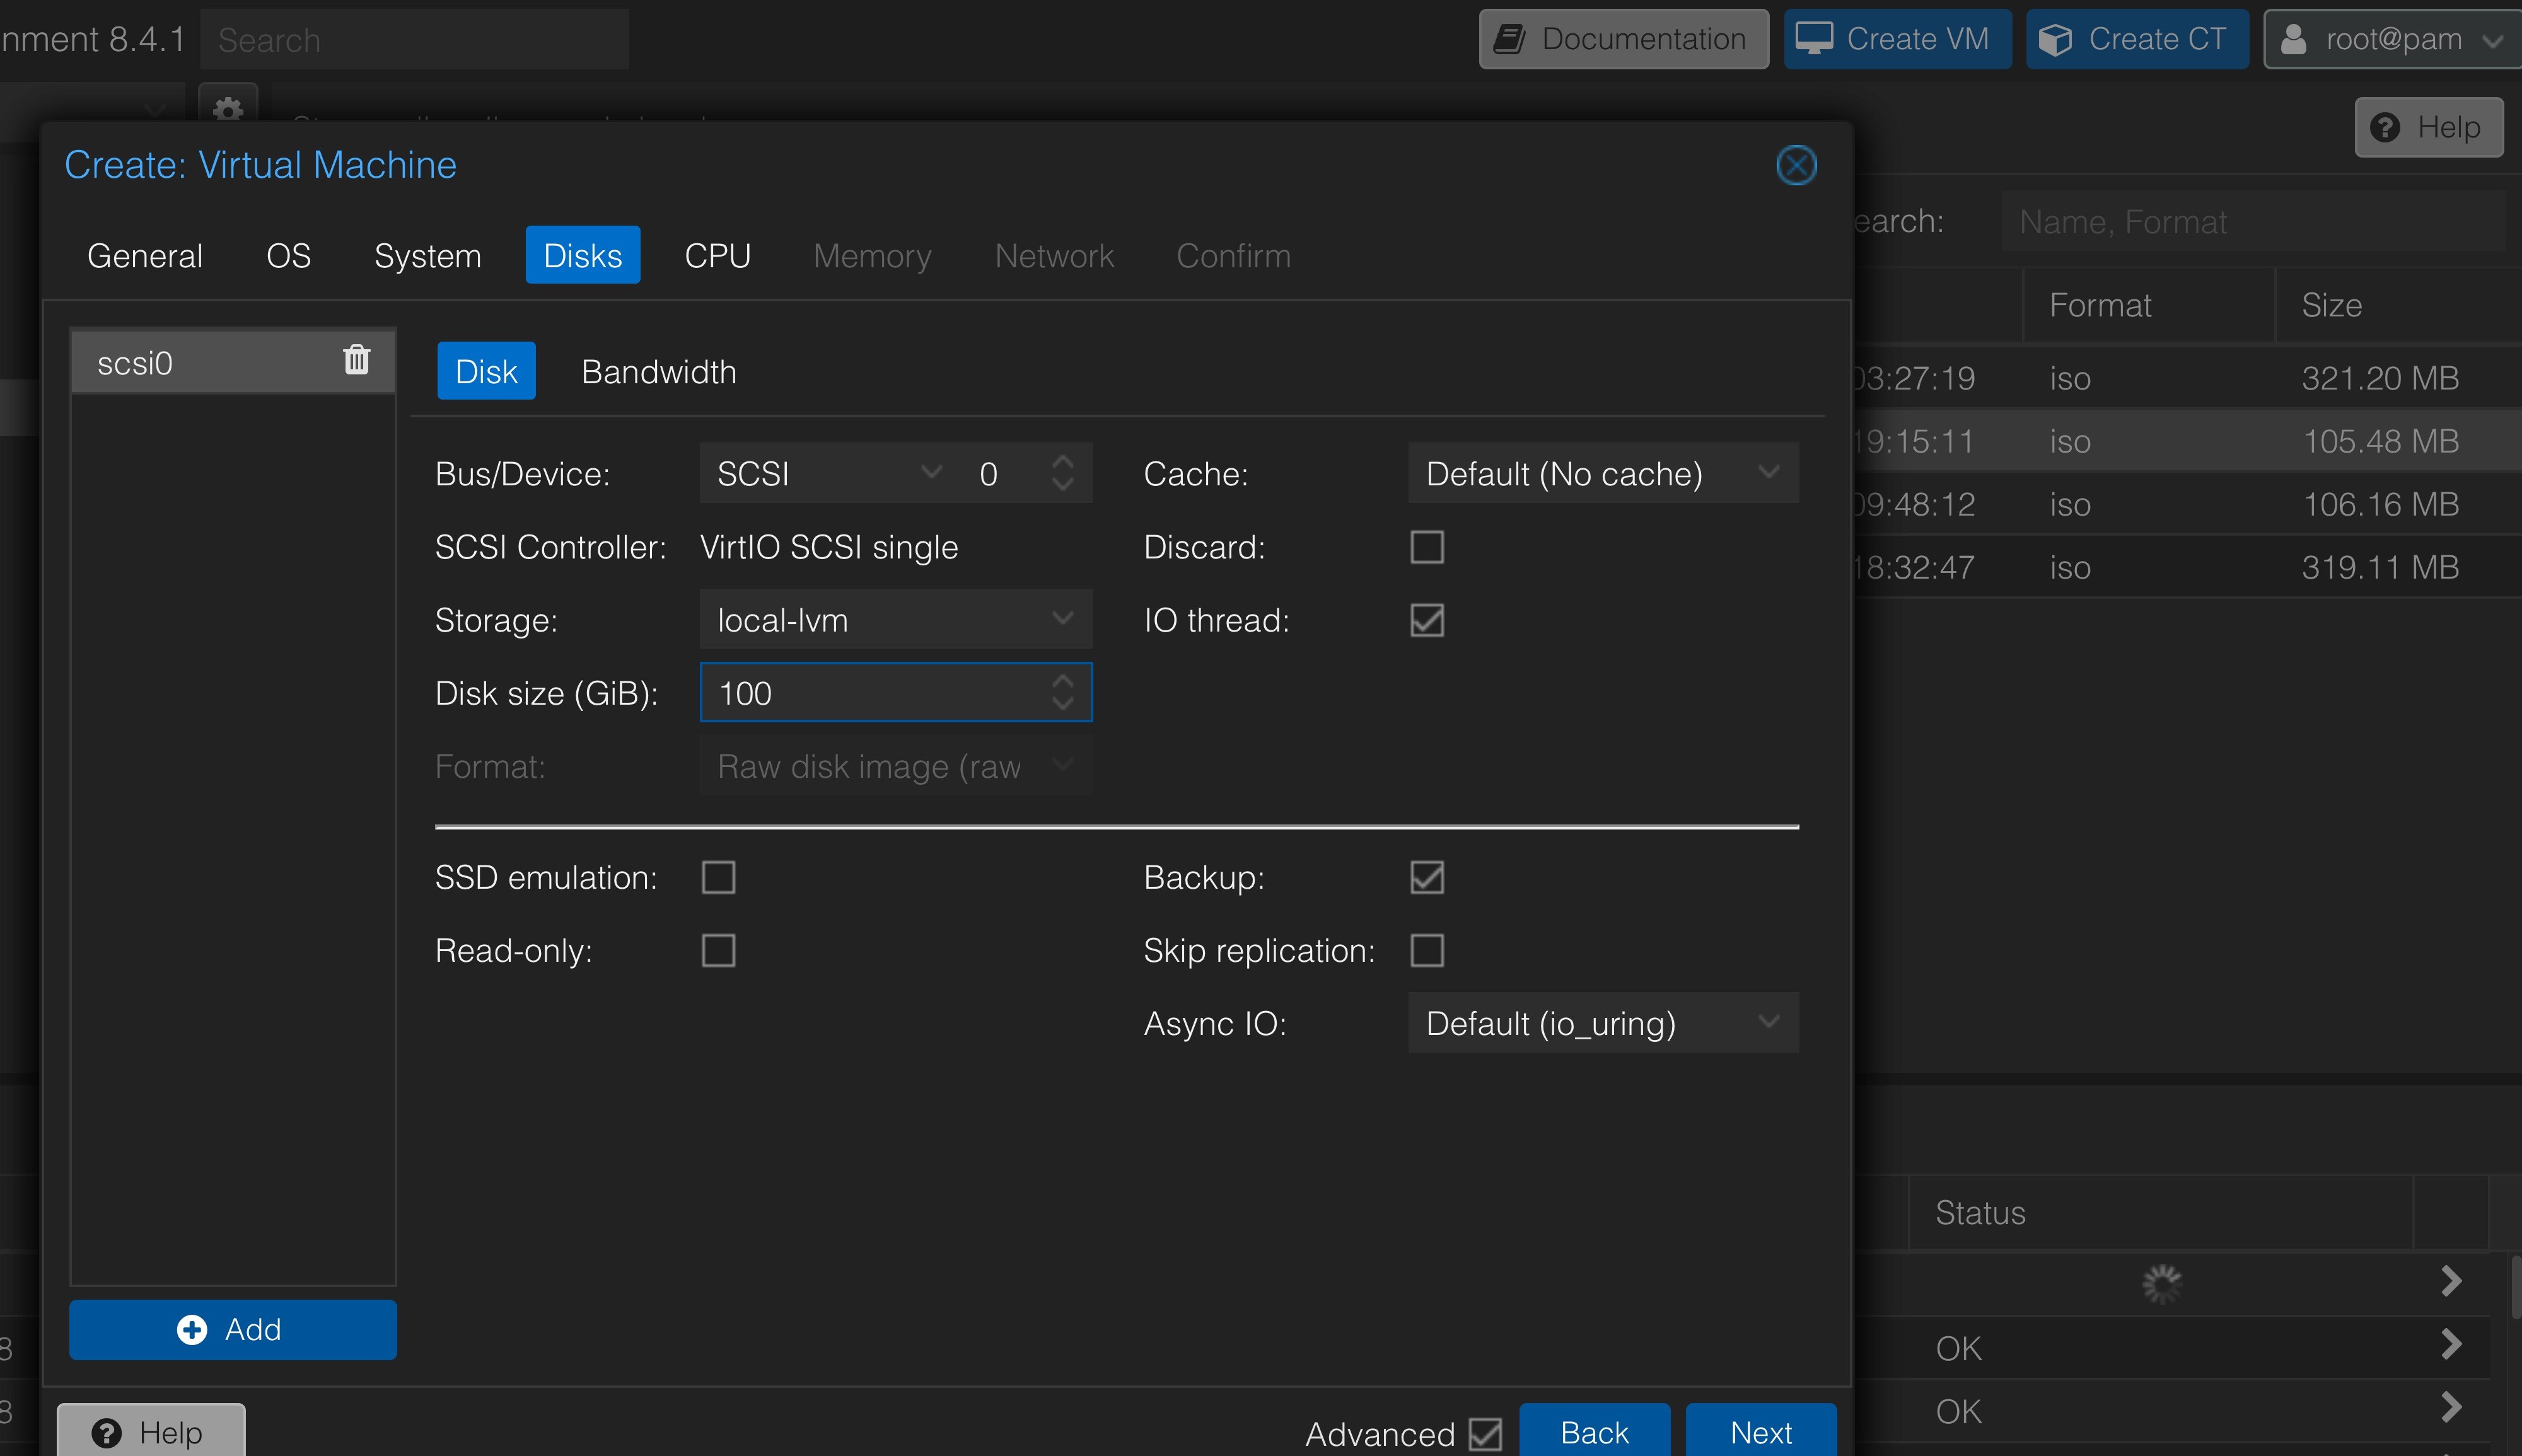
\includegraphics[width=1\textwidth]{figures/talos-install-5.jpg}
    \caption{Instalasi Talos OS 4}
\end{figure}
\begin{figure}[!htbp]
    5. Pada bagian CPU. Cukup merubah cores menjadi 2 atau 4 sesuai spesifikasi mesin yang diinginkan
    \centering
    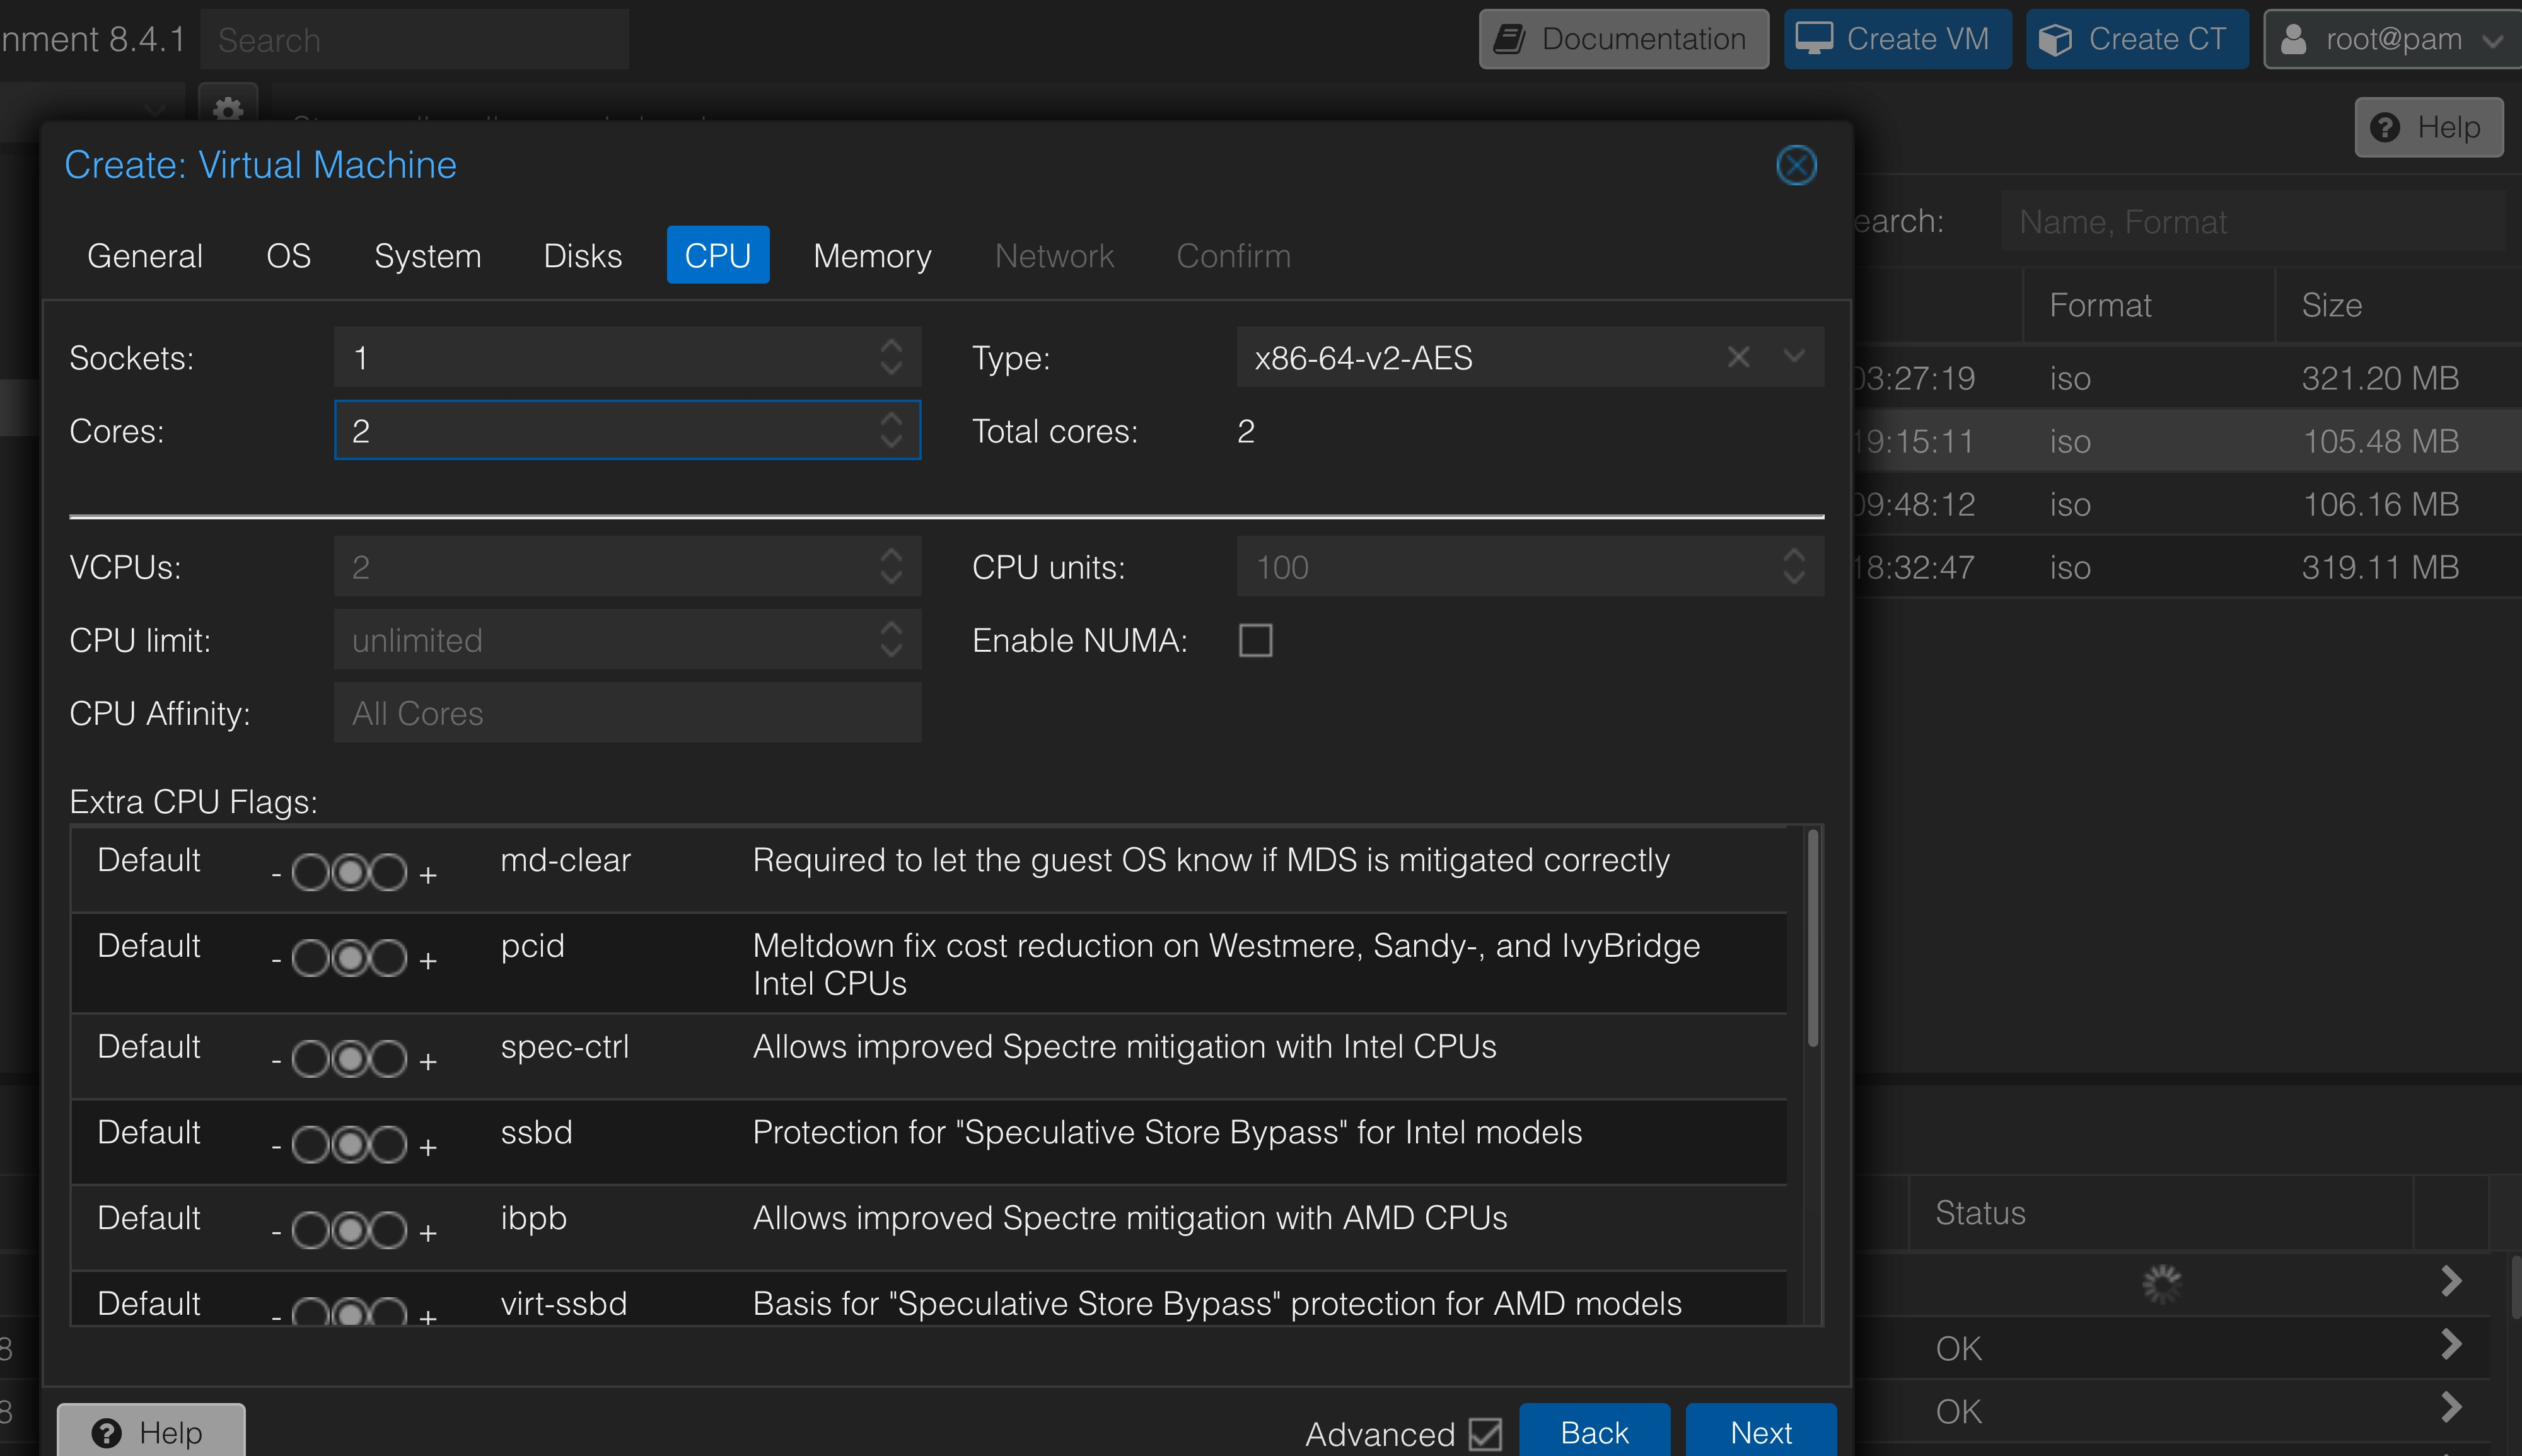
\includegraphics[width=1\textwidth]{figures/talos-install-6.jpg}
    \caption{Instalasi Talos OS 5}
\end{figure}
\begin{figure}[!htbp]
    6. Pada bagian memory. Isikan memory sesuai yang dinginkan dengan minimal 8192 MiB
    \centering
    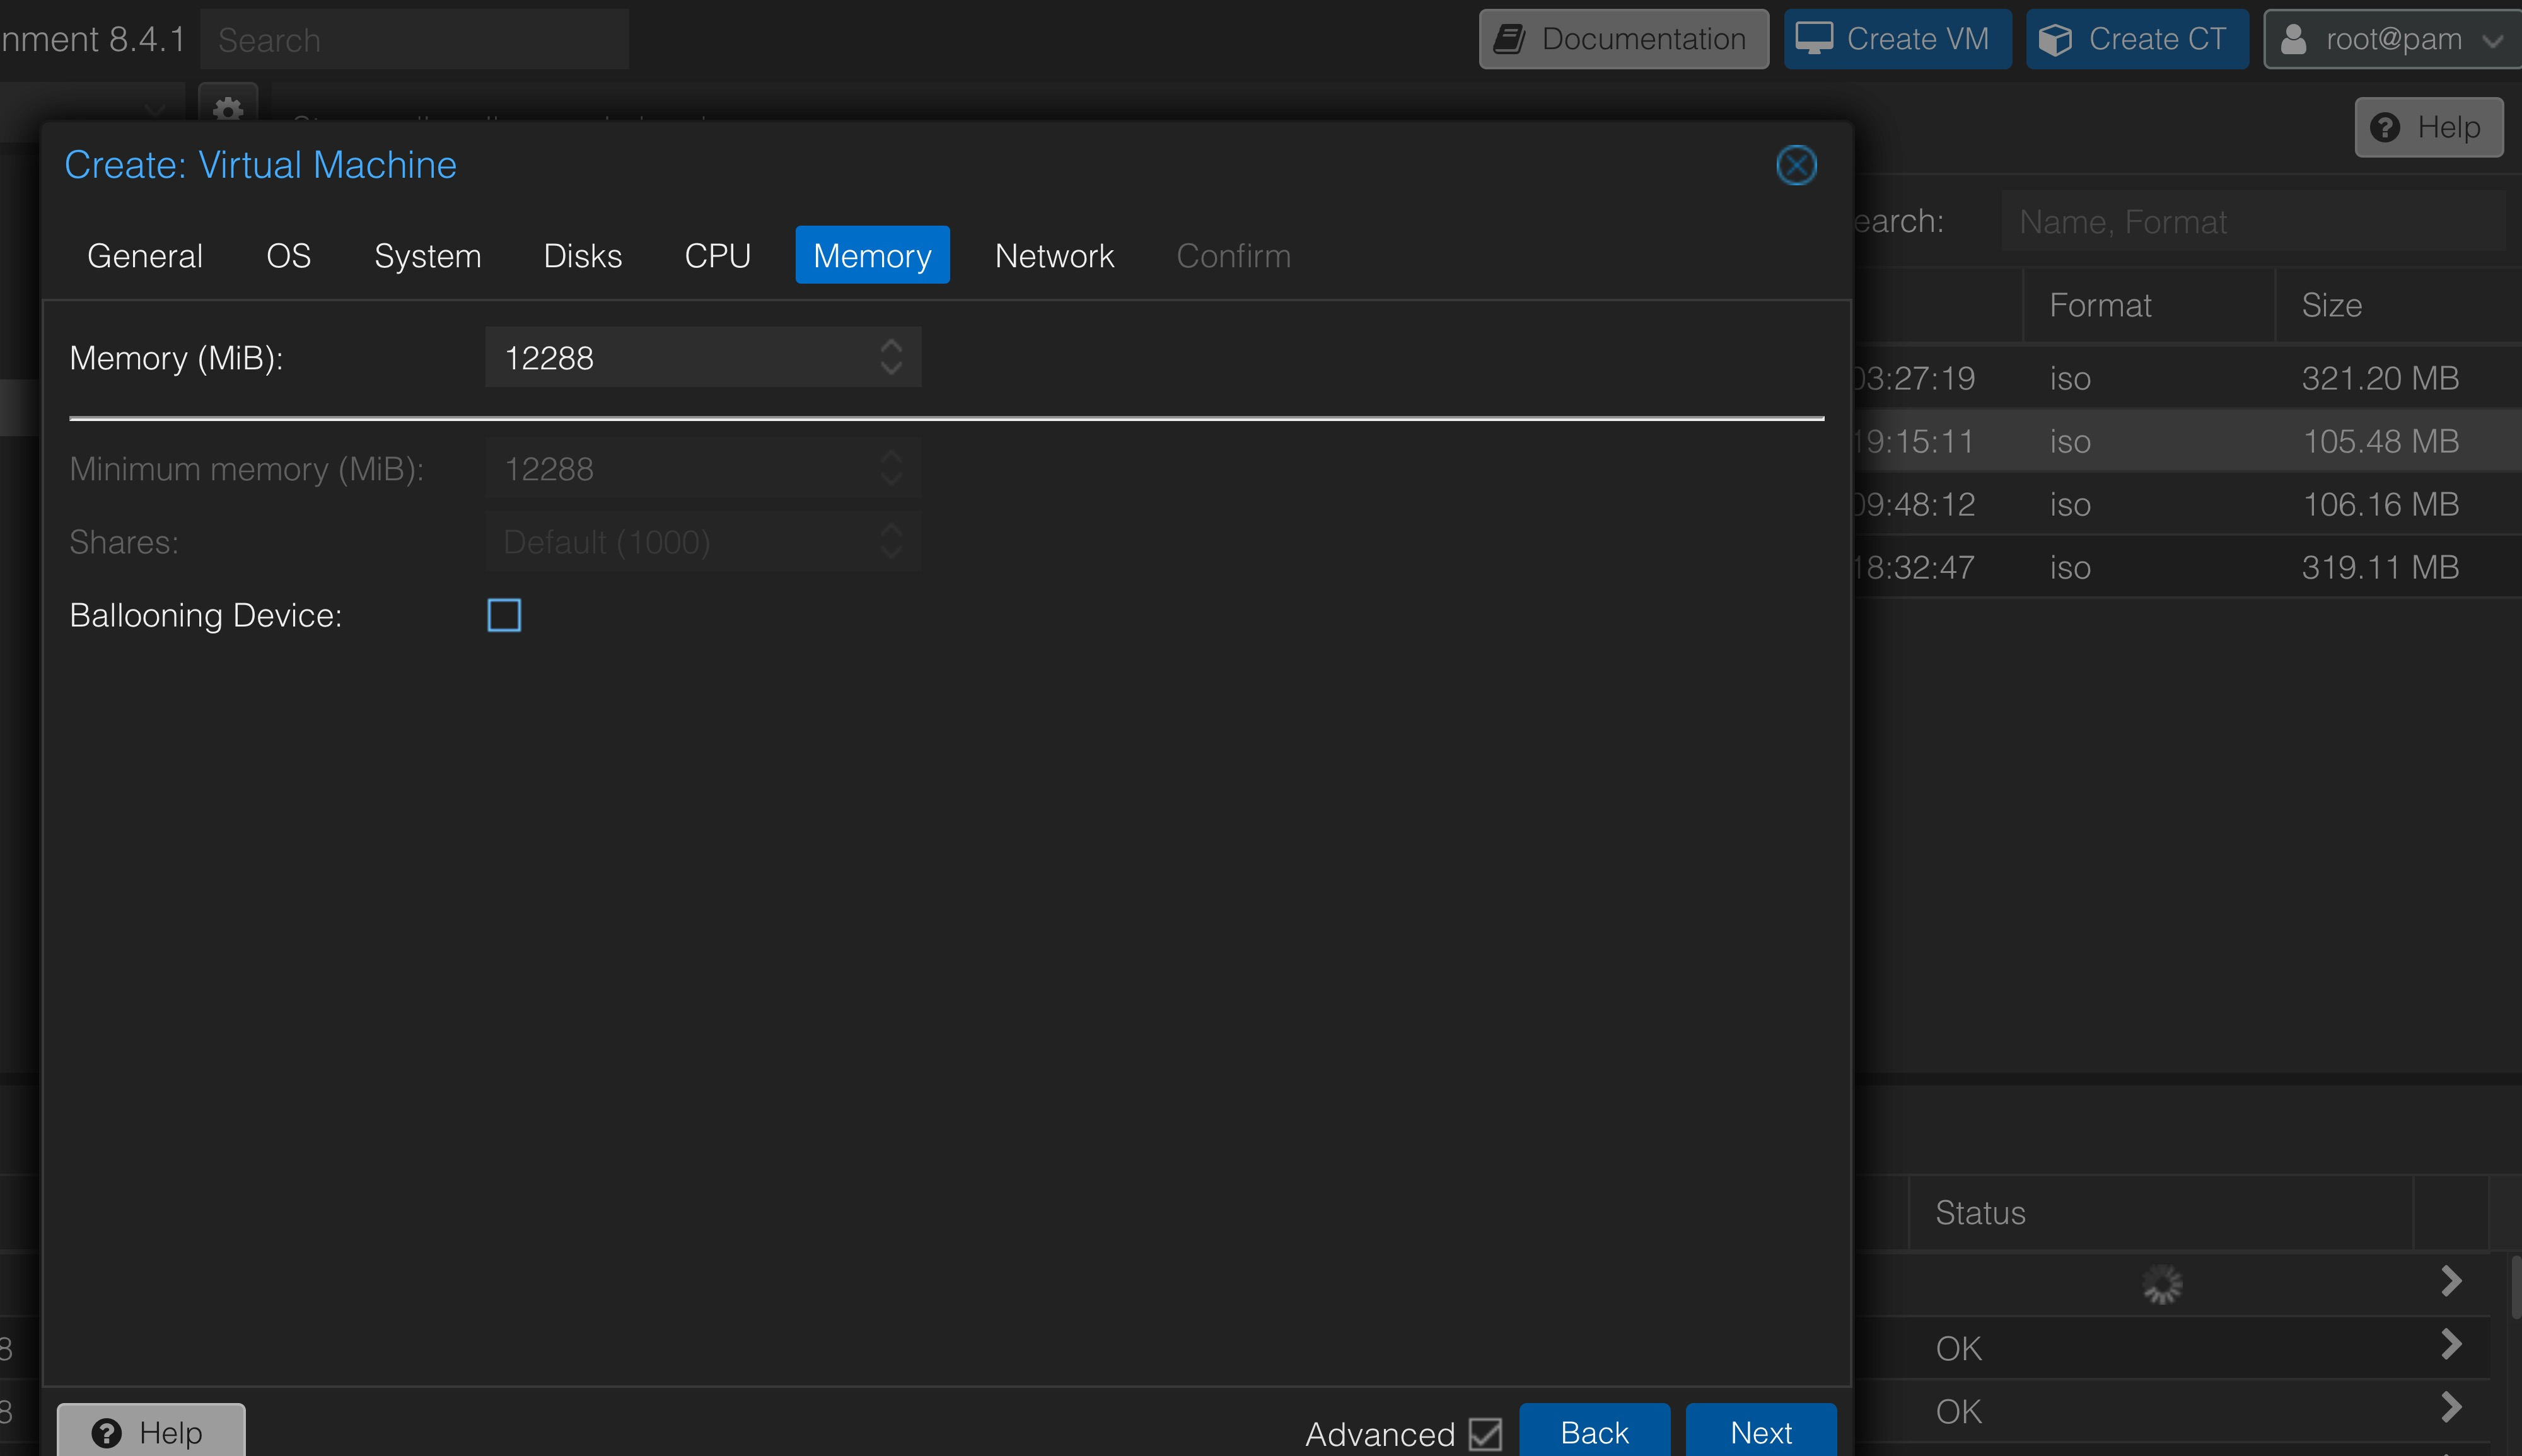
\includegraphics[width=1\textwidth]{figures/talos-install-7.jpg}
    \caption{Instalasi Talos OS 6}
\end{figure}
\begin{figure}[!htbp]
    7. Pada bagian Network. Silahkan klik next
    \centering
    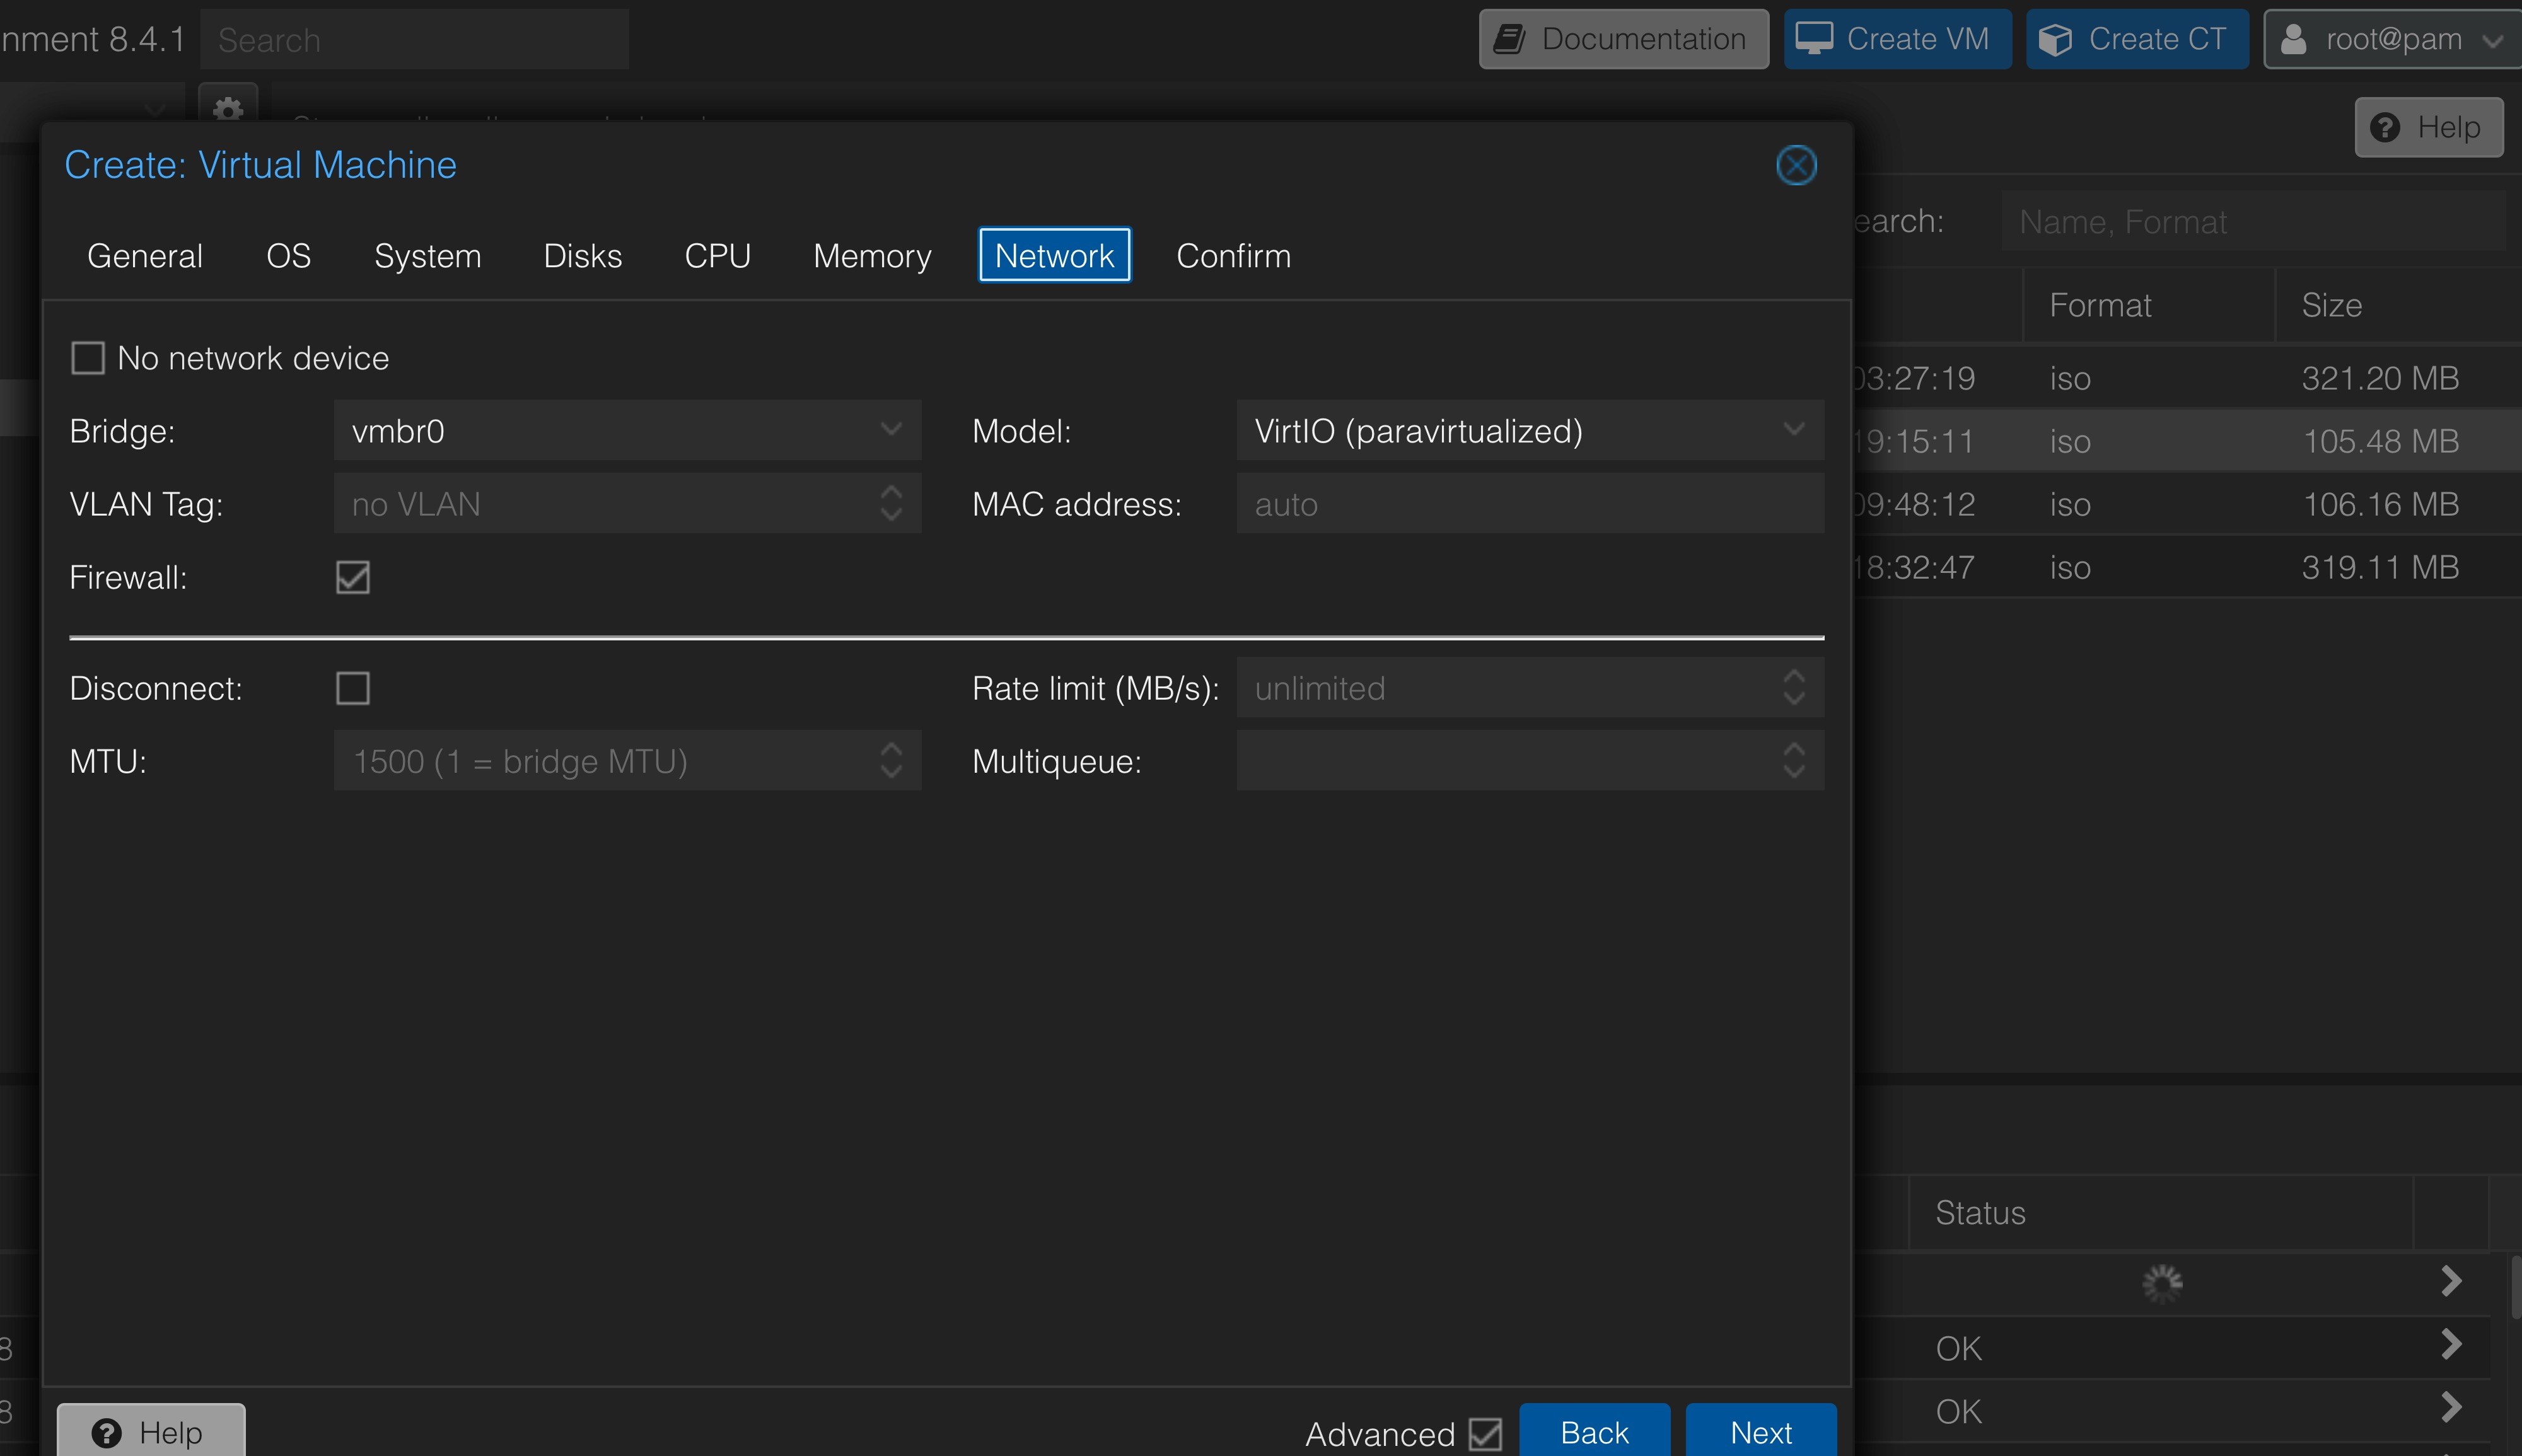
\includegraphics[width=1\textwidth]{figures/talos-install-8.jpg}
    \caption{Instalasi Talos OS 7}
\end{figure}
\begin{figure}[!htbp]
    8. Pada bagian confirm. Centang "Start After Created" lalu Finish
    \centering
    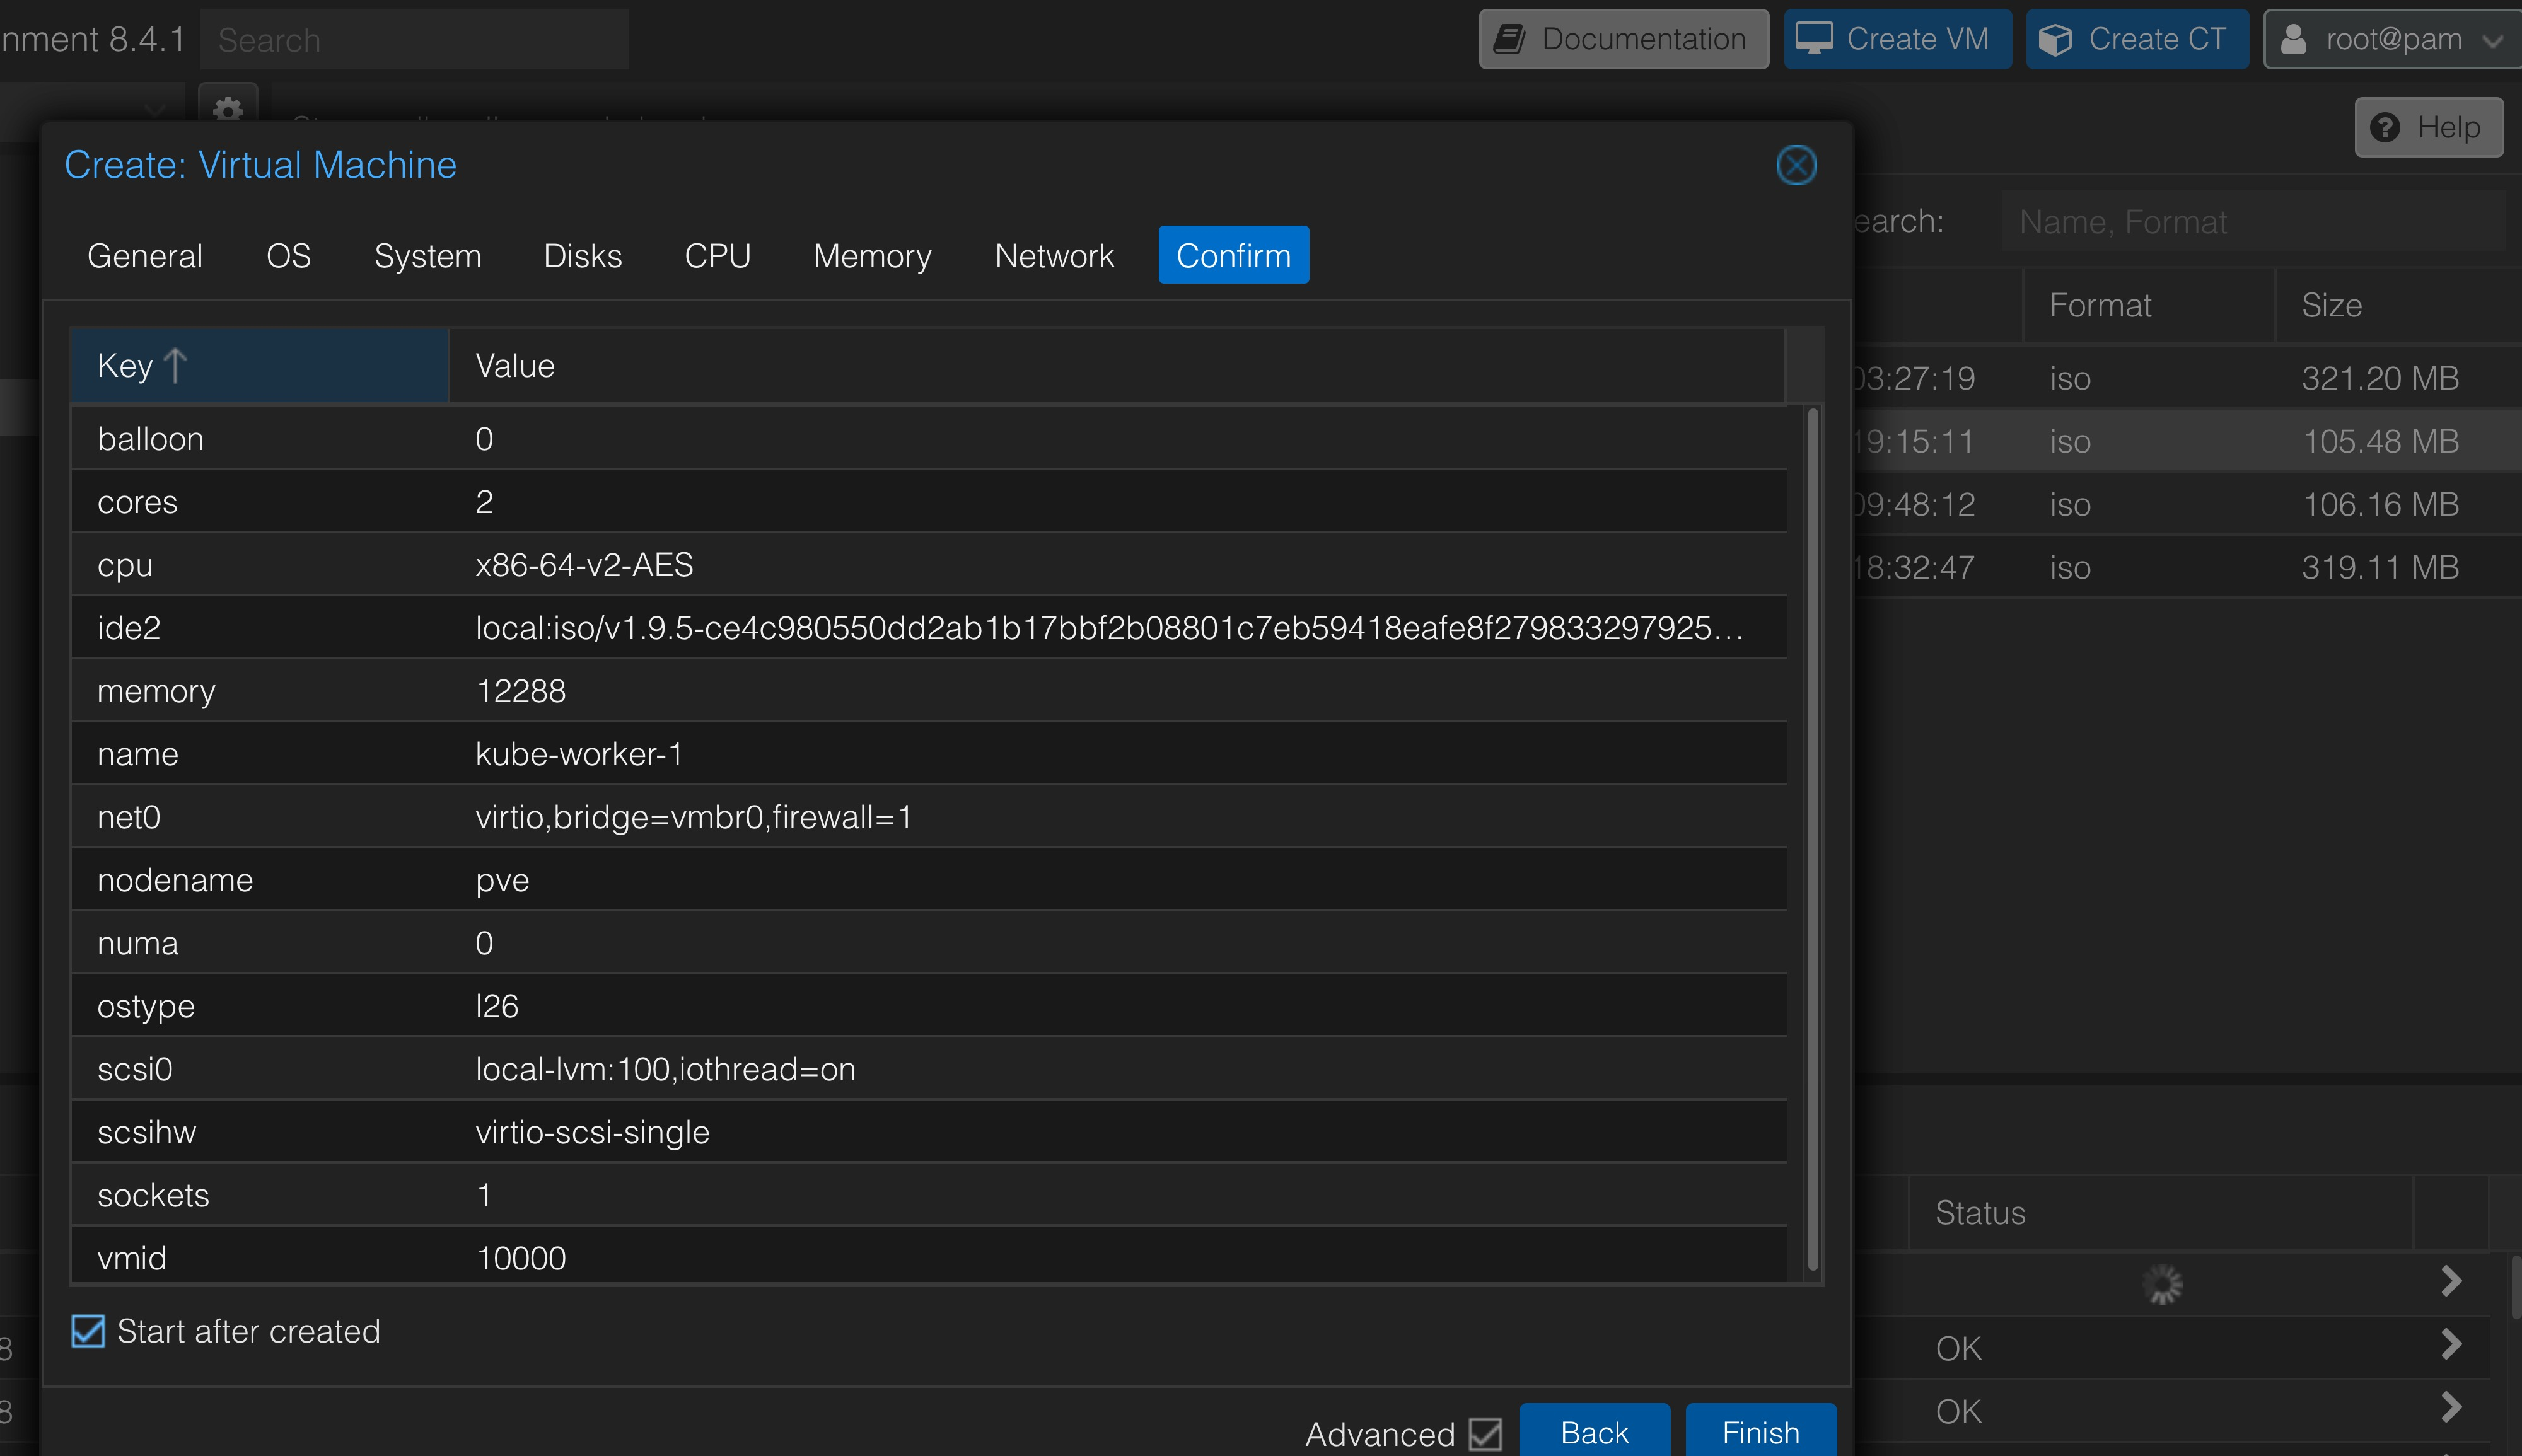
\includegraphics[width=1\textwidth]{figures/talos-install-9.jpg}
    \caption{Instalasi Talos OS 8}
\end{figure}
\begin{figure}[!htbp]
    10. Ketika Talos OS Sudah berjalan terminal Talos OS akan tampak seperti ini
    \centering
    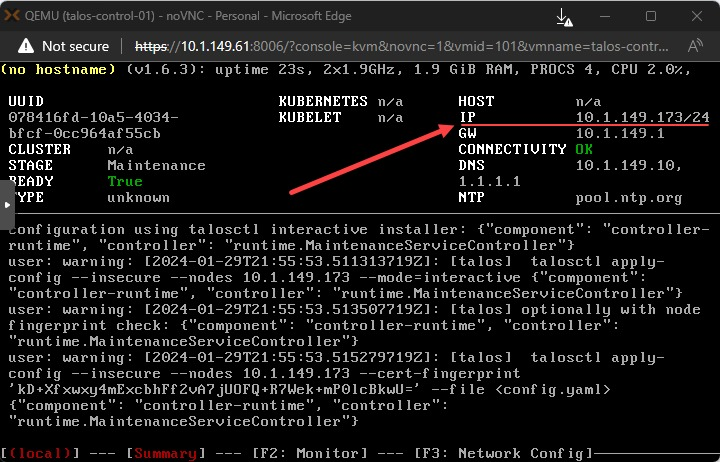
\includegraphics[width=1\textwidth]{figures/talos-install-10.jpg}
    \caption{Instalasi Talos OS 9}
\end{figure}
\newpage

\subsection{Pengkodean Instalasi Kubernetes Script}
Tahap ini adalah tahap untuk instalasi Kubernetes pada Talos OS. Disini peneliti akan menggunakan deklaratif yaml yang akan mengautomatisasi instalasi kubernetes pada Talos OS.
Instalasi Kubernetes pada Talos OS sendiri mengikuti panduan dari pedoman yang terdapat pada website Talos OS \url{https://www.talos.dev/v1.9.5/introduction/getting-started/}

\begin{table}[!htbp]
    \begin{lstlisting}[language=yaml, basicstyle=\footnotesize\ttfamily]
version: '3'
tasks:
  talos:
    desc: Bootstrap the Talos cluster
    dir: '{{.TALOS_DIR}}'
    cmds:
      - '[ -f talsecret.sops.yaml ] || talhelper gensecret | sops --filename-override talos/talsecret.sops.yaml --encrypt /dev/stdin > talsecret.sops.yaml'
      - talhelper genconfig
      - talhelper gencommand apply --extra-flags="--insecure" | bash
      - until talhelper gencommand bootstrap | bash; do sleep 10; done
      - until talhelper gencommand kubeconfig --extra-flags="{{.ROOT_DIR}} --force" | bash; do sleep 10; done
\end{lstlisting}
    \caption{Konfigurasi script instalasi Kubernetes cluster pada Talos OS}
    \label{tab:yaml-code}
\end{table}
\begin{table}[!htbp]
    \begin{lstlisting}[language=yaml, basicstyle=\footnotesize\ttfamily]
clusterName: kubernetes
endpoint: https://192.168.0.250:6443
...
nodes:
  - hostname: "kube-cp-1"
    ipAddress: "192.168.0.200"
    installDisk: "/dev/sda"
    machineSpec:
    controlPlane: true
    networkInterfaces:
      - deviceSelector:
          hardwareAddr: "de:ad:be:ef:00:01"
        addresses:
          - "192.168.0.200/24"
        routes:
          - network: "0.0.0.0/0"
            gateway: "192.168.0.1"
        mtu: 1500
        vip:
          ip: "192.168.0.250"
  - hostname: "kube-worker-1"
    ipAddress: "192.168.0.201"
    installDisk: "/dev/sda"
    machineSpec:
    controlPlane: false
    networkInterfaces:
      - deviceSelector:
          hardwareAddr: "de:ad:be:ef:00:02"
        dhcp: false
        addresses:
          - "192.168.0.201/24"
        routes:
          - network: "0.0.0.0/0"
            gateway: "192.168.0.1"
        mtu: 1500
\end{lstlisting}
    \caption{Konfigurasi script instalasi Kubernetes cluster pada Talos OS}
    \label{tab:yaml-code-2}
\end{table}
\newpage
Setelah dilakukan instalasi Kubernetes cluster pada Talos OS tampilan terminal akan menampilkan nama cluster
dan juga sudah tidak menampilan status Stage: Maintenance seperti Gambar 4.16.
\begin{figure}[!ht]
    \centering
    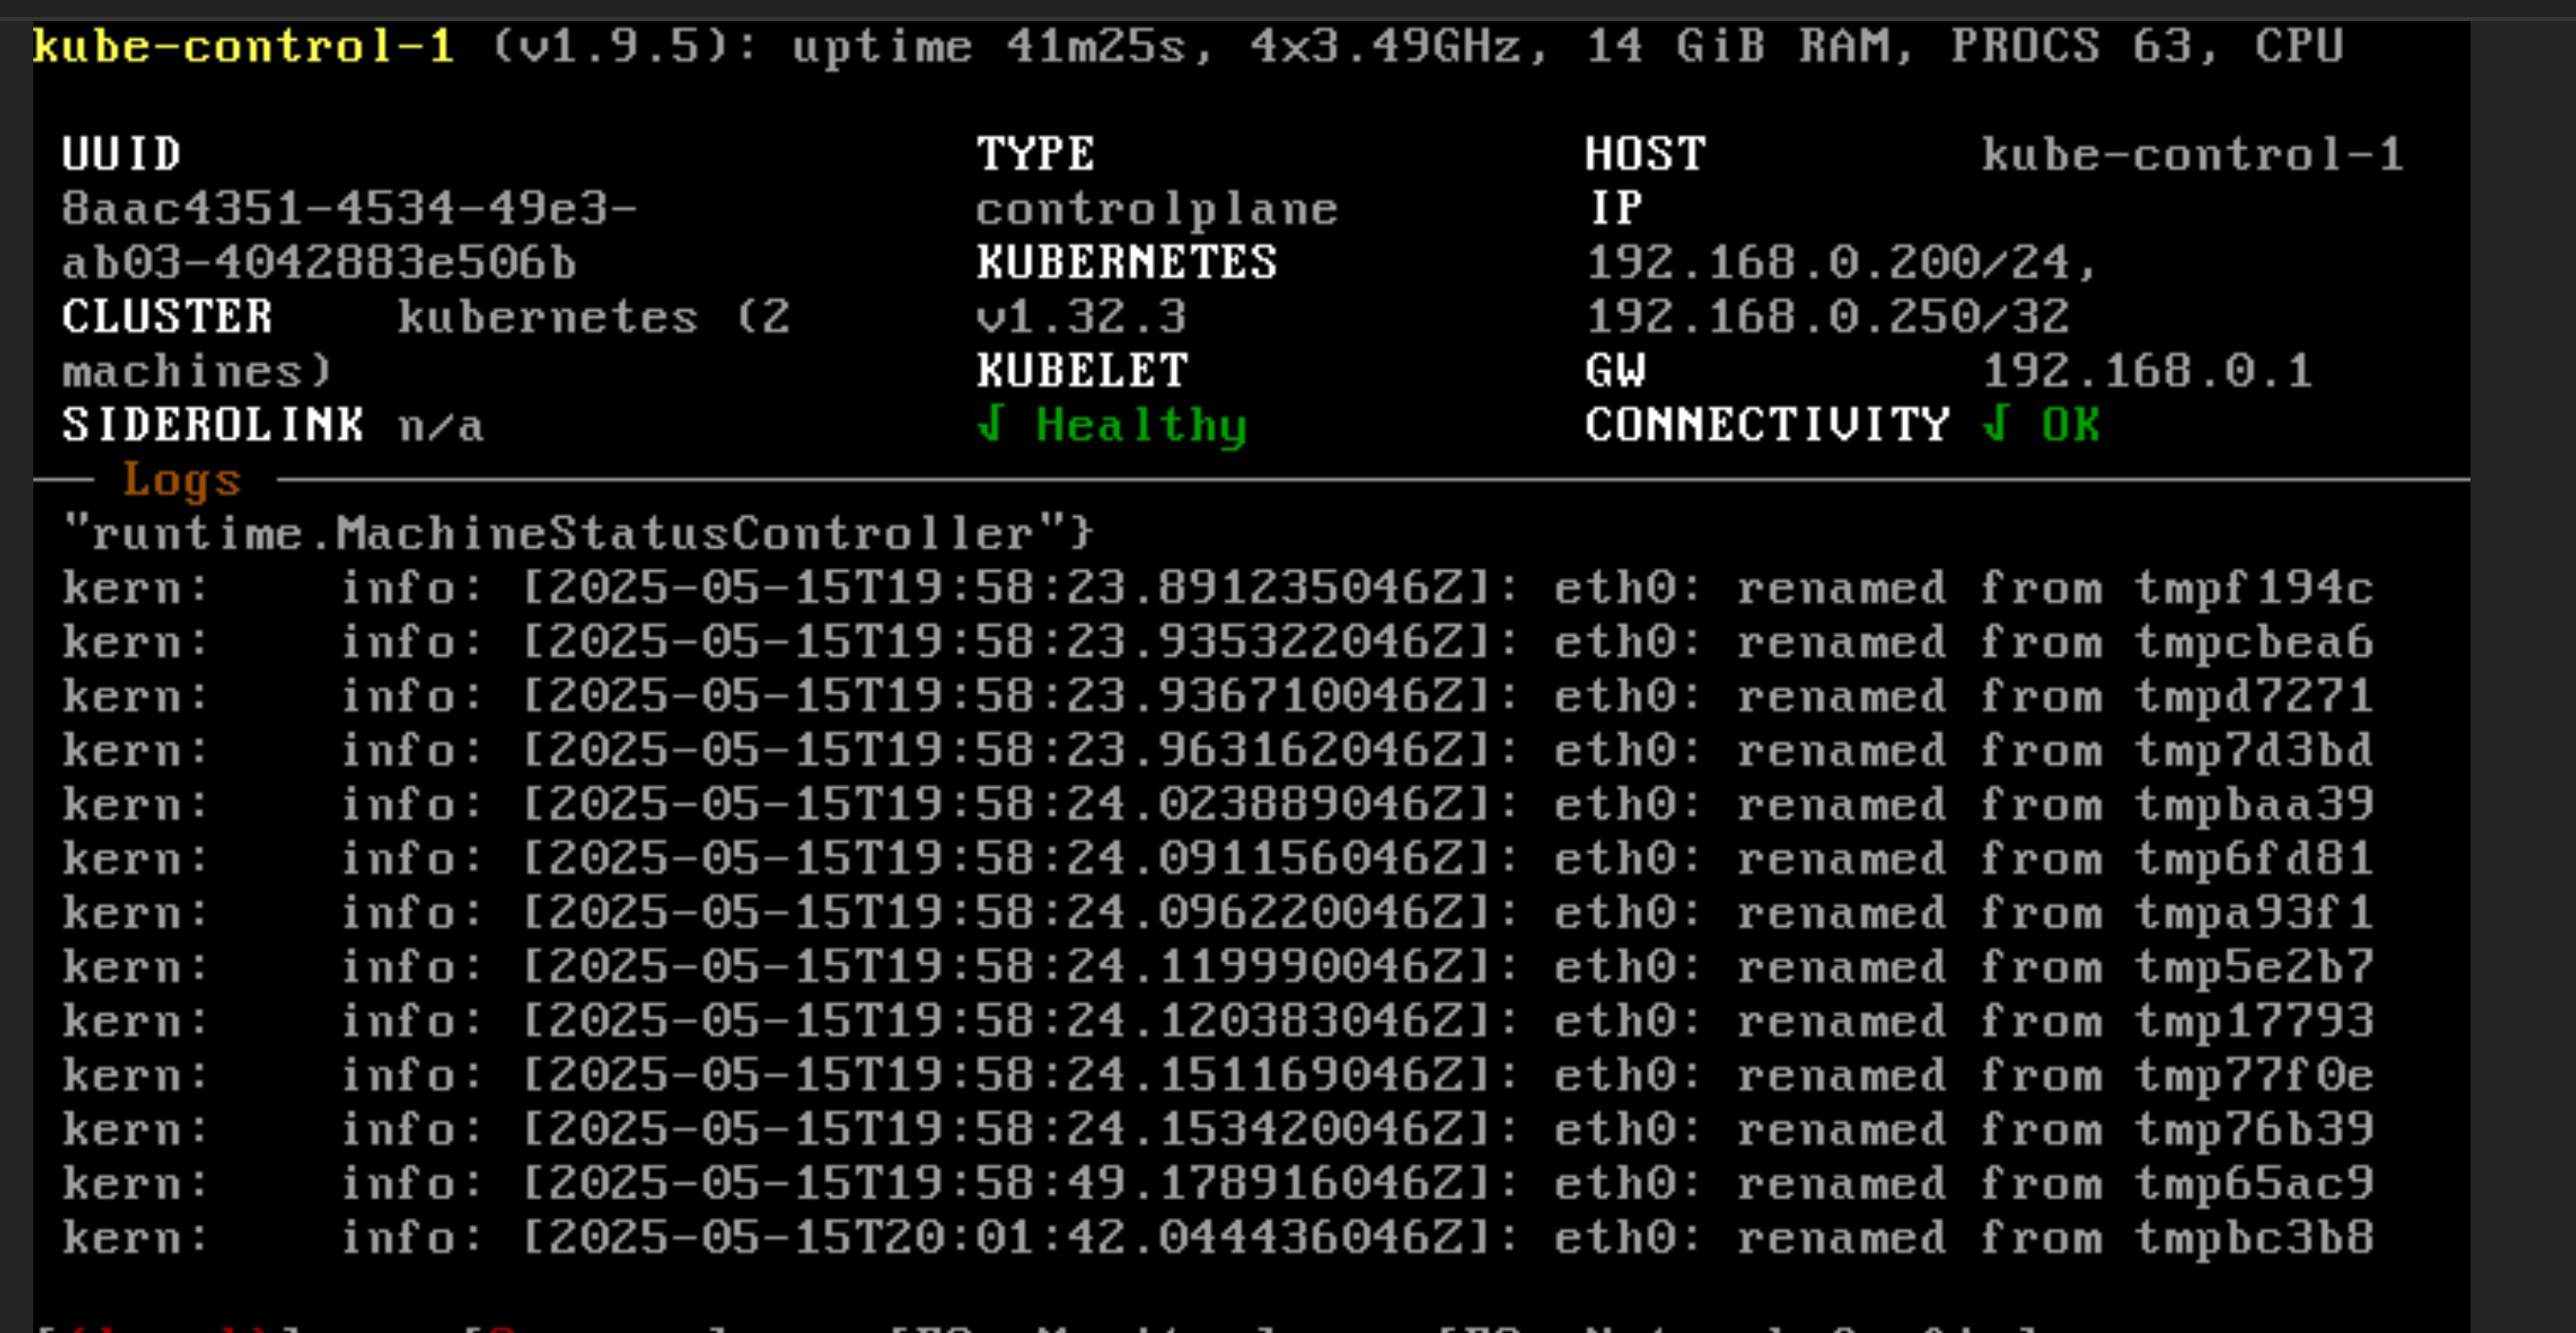
\includegraphics[width=1\textwidth]{figures/talos-install-11.jpg}
    \caption{Tampilan Talos OS setelah instalasi kubernetes cluster}
\end{figure}
\newpage
Setelah instalasi kubernetes pada Talos OS dilakukan maka kita dapat mengakses kubernetes cluster tersebut menggunakan cli kubectl.
Sebagai contoh saya mempunyai aplikasi yang menampilkan informasi header pada browser pada \url{echo.zeinfahrozi.my.id}
\begin{figure}[!ht]
    \centering
    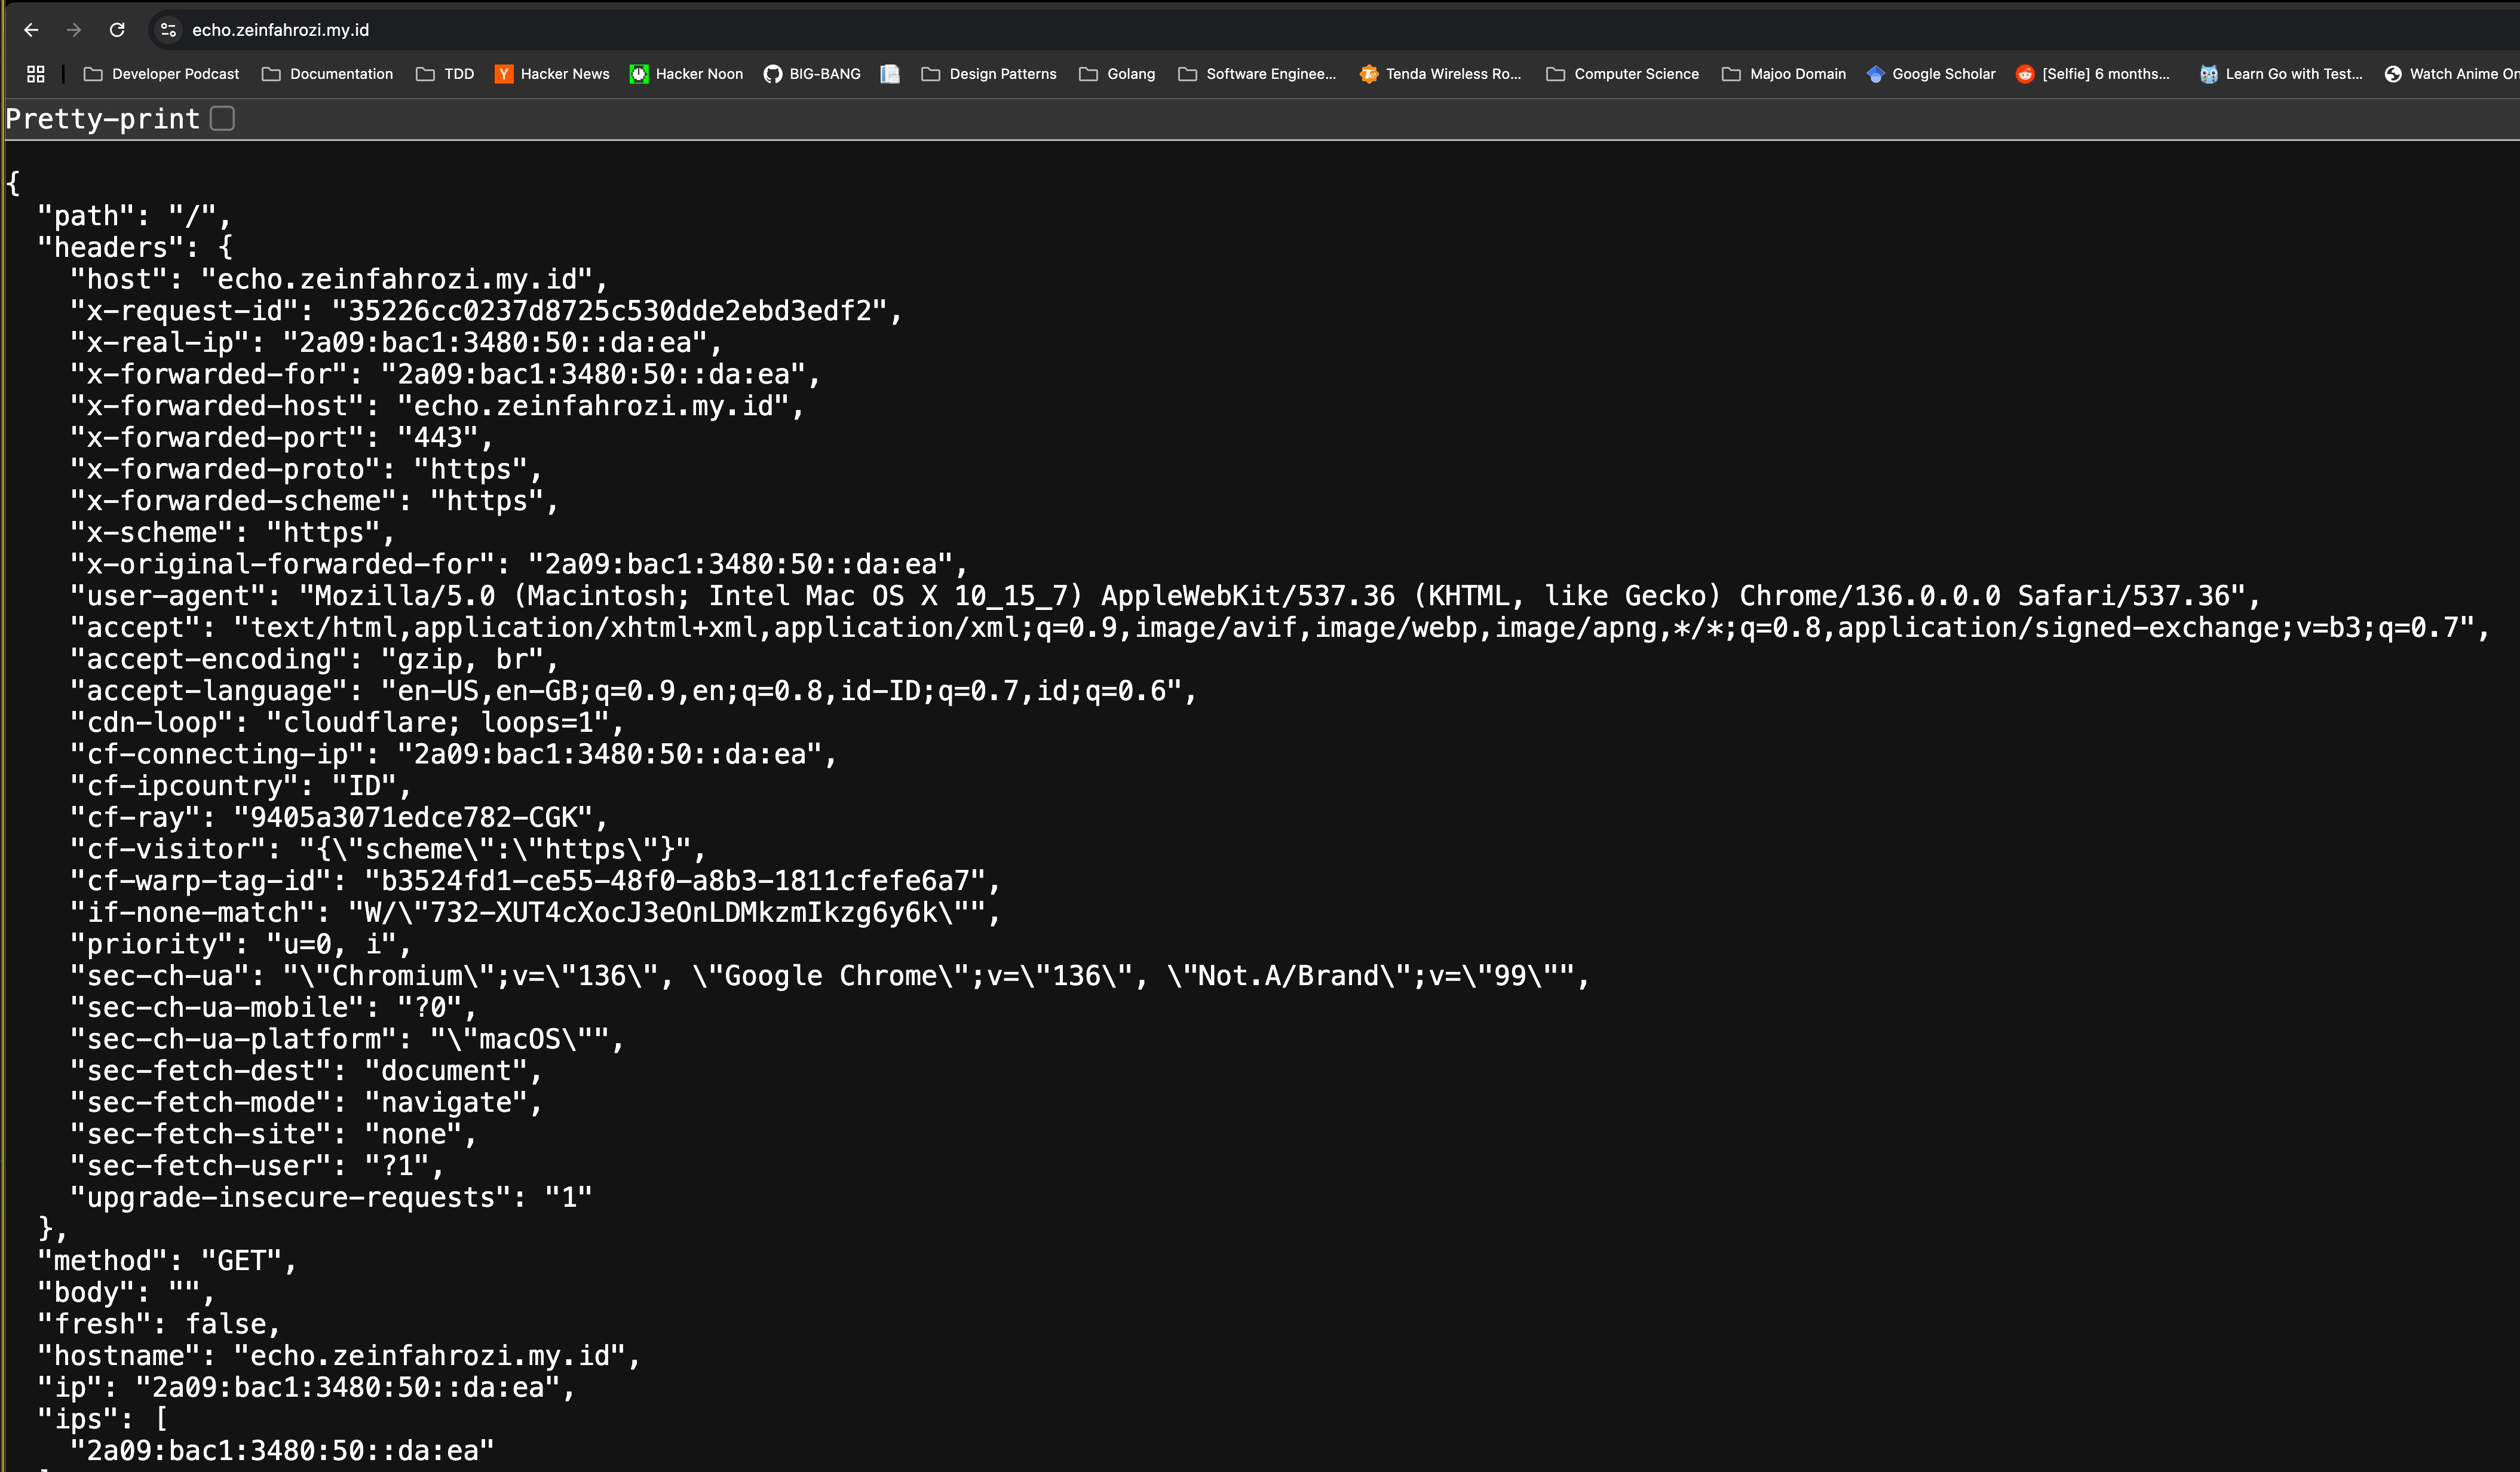
\includegraphics[width=1\textwidth]{figures/echo-web.jpg}
    \caption{Tampilan echo.zeinfahrozi.my.id pada browser}
\end{figure}
\section{Implementasi ArgoCD pada cluster kubernetes}
Tahap ini merupakan instalasi instance ArgoCD itu sendiri pada kubernetes cluster yang sudah dibuat sebelumnya. ArgoCD dipasang menggunakan Helm chart dengan konfigurasi kustom yang disesuaikan dengan kebutuhan lingkungan produksi.

Berikut adalah contoh perintah untuk menginstal ArgoCD menggunakan Helm:

\begin{lstlisting}[language=bash, basicstyle=\footnotesize\ttfamily]
# Menambahkan repo ArgoCD
helm repo add argo https://argoproj.github.io/argo-helm
helm repo update

# Membuat namespace untuk ArgoCD
kubectl create namespace argocd

# Menginstal ArgoCD dengan Helm
helm upgrade --install argocd argo/argo-cd \
  --namespace argocd \
  --values values.sops.yaml \
  --wait
\end{lstlisting}

\subsection{Instalasi ArgoCD}
ArgoCD diinstal menggunakan Helm dengan nilai-nilai kustom yang didefinisikan dalam file konfigurasi. Berikut adalah contoh konfigurasi \texttt{values.sops.yaml} yang digunakan:

\begin{lstlisting}[language=yaml, basicstyle=\footnotesize\ttfamily]
# values.sops.yaml
crds:
  install: true

global:
  domain: argo.zeinfahrozi.my.id

configs:
  params:
    server.insecure: true
  cm:
    statusbadge.enabled: true
    kustomize.buildOptions: --enable-alpha-plugins --enable-exec
    helm.valuesFileSchemes: >-
      secrets+gpg-import,secrets+gpg-import-kubernetes,
      secrets+age-import,secrets+age-import-kubernetes,
      secrets,secrets+literal,https
    resource.exclusions: |
      - apiGroups:
          - cilium.io
        kinds:
          - CiliumIdentity
        clusters:
          - "*"
\end{lstlisting}

Beberapa konfigurasi penting yang diterapkan:

\begin{itemize}
    \item ArgoCD diakses melalui domain \texttt{argo.zeinfahrozi.my.id}
    \item Mode \texttt{insecure} diaktifkan untuk pengembangan
    \item Fitur status badge diaktifkan untuk memantau status aplikasi
    \item Dukungan untuk multiple value files dengan skema yang berbeda
    \item Eksklusi sumber daya tertentu seperti CiliumIdentity dari manajemen ArgoCD
\end{itemize}

\subsection{Konfigurasi High Availability}
Untuk memastikan ketersediaan tinggi, komponen-komponen kritis ArgoCD dikonfigurasi dengan multiple replica:

\begin{itemize}
    \item ArgoCD Server: 2 replica
    \item ArgoCD Controller: 2 replica
    \item Dex Server: 2 replica
\end{itemize}

\subsection{Integrasi dengan Monitoring}
ArgoCD terintegrasi dengan stack monitoring yang sudah ada di cluster melalui ServiceMonitor untuk memantau metrik dari komponen-komponennya:

\begin{itemize}
    \item ArgoCD Server metrics
    \item ArgoCD Controller metrics
    \item Dex Server metrics
    \item Redis metrics
\end{itemize}

\subsection{Manajemen Aplikasi}
Setelah ArgoCD terinstal, aplikasi-aplikasi dapat dikelola menggunakan GitOps. Setiap aplikasi didefinisikan sebagai kustom resource Kubernetes yang mereferensikan repositori Git yang berisi manifest Kubernetes. ArgoCD akan secara otomatis melakukan sinkronisasi antara status yang diinginkan (yang didefinisikan di Git) dengan status aktual di cluster.

\subsection{Keamanan}
Beberapa aspek keamanan yang diterapkan pada instalasi ArgoCD ini antara lain:

\begin{itemize}
    \item Penggunaan HTTPS untuk akses web UI
    \item Integrasi dengan Dex untuk autentikasi
    \item Pembatasan akses berbasis peran (RBAC)
    \item Penyimpanan rahasia yang aman menggunakan SOPS
\end{itemize}

Dengan konfigurasi ini, ArgoCD siap digunakan untuk mengelola aplikasi secara deklaratif menggunakan prinsip GitOps, di mana semua perubahan konfigurasi dilakukan melalui pull request dan version control system.

\section{Implementasi Cloudflare Tunnel}
Cloudflare Tunnel digunakan untuk mengekspos layanan dalam cluster ke internet dengan aman tanpa perlu membuka port firewall. Berikut adalah langkah-langkah implementasinya:

1. **Persiapan**
- Memiliki akun Cloudflare
- Mendaftarkan domain yang akan digunakan
- Mengatur DNS di Cloudflare

2. **Instalasi Cloudflare Tunnel**
Cloudflare Tunnel diinstal menggunakan ArgoCD dengan konfigurasi sebagai berikut:

\begin{lstlisting}[language=yaml, basicstyle=\footnotesize\ttfamily]
# cloudflared.yaml
apiVersion: argoproj.io/v1alpha1
kind: Application
metadata:
     name: cloudflared
     namespace: argo-system
   spec:
     project: kubernetes
     sources:
       - repoURL: "https://github.com/mozarik/zein-home-lab.git"
         path: kubernetes/apps/network/cloudflared
         targetRevision: main
     destination:
       name: in-cluster
       namespace: network
     syncPolicy:
       automated:
         prune: true
         selfHeal: true
\end{lstlisting}

3. **Konfigurasi Tunnel**
Setelah terinstal, Cloudflare Tunnel perlu dikonfigurasi untuk meneruskan lalu lintas ke layanan dalam cluster. Berikut contoh konfigurasi untuk mengekspos ArgoCD:

\begin{lstlisting}[language=yaml, basicstyle=\footnotesize\ttfamily]
   # config.yaml
   tunnel: <tunnel-id>
   credentials-file: /etc/cloudflared/credentials.json
   ingress:
     - hostname: argo.zeinfahrozi.my.id
       service: http://argocd-server.argocd.svc.cluster.local:80
     - service: http_status:404
   \end{lstlisting}

\subsection{Konfigurasi Git Repository}
Git repository digunakan sebagai sumber kebenaran (source of truth) untuk konfigurasi infrastruktur. Repository yang digunakan adalah \url{https://github.com/mozarik/zein-home-lab} dengan struktur sebagai berikut:


Alur kerja GitOps yang diterapkan:
1. Perubahan konfigurasi dilakukan melalui pull request
2. Setelah pull request disetujui dan digabungkan ke branch main
3. ArgoCD secara otomatis mendeteksi perubahan dan melakukan sinkronisasi dengan cluster

\subsection{Integrasi dengan GitHub Actions}
Untuk memastikan kualitas kode dan keamanan, diterapkan GitHub Actions workflow yang akan:
1. Melakukan linting pada file konfigurasi Kubernetes
2. Melakukan validasi dengan kubeval
3. Melakukan pengecekan keamanan dengan kubesec

Contoh workflow GitHub Actions:

\begin{lstlisting}[language=yaml, basicstyle=\footnotesize\ttfamily]
name: Lint and Validate

on:
  push:
    branches: [ main ]
  pull_request:
    branches: [ main ]

jobs:
  lint-validate:
    runs-on: ubuntu-latest
    steps:
      - uses: actions/checkout@v3
      
      - name: Lint Kubernetes files
        uses: azure/k8s-manifests-base@v1
        with:
          action: lint
          files: '**/*.yaml'

      - name: Validate Kubernetes files
        uses: azure/k8s-manifests-base@v1
        with:
          action: validate
          files: '**/*.yaml'
\end{lstlisting}

Dengan konfigurasi ini, seluruh perubahan infrastruktur dapat dilacak melalui riwayat Git, dan proses deployment menjadi lebih terotomatisasi dan konsisten.

\section{Testing}
Setelah menyelesaikan tahap instalasi dan konfigurasi infrastruktur, langkah selanjutnya adalah melakukan pengujian untuk memastikan seluruh komponen berfungsi seperti yang diharapkan. Pengujian ini mencakup beberapa aspek penting termasuk fungsionalitas Kubernetes cluster, integrasi ArgoCD, serta alur kerja GitOps yang telah diterapkan. Melalui pengujian menyeluruh ini, diharapkan dapat dievaluasi sejauh mana solusi yang dibangun mampu memenuhi kebutuhan pengembangan dan operasional aplikasi secara efisien.

\subsection{Pengujian (Testing)}\label{sec:bab4_pengujian}
Pengujian black-box testing yang dilakukan terhadap sistem pada tahap ini menggunakan metode validasi (validation). Metode validasi yang digunakan dalam melakukan pengujian ini berfungsi untuk mengetahui valid atau tidaknya sebuah fungsi dari sistem yang dibangun. Melakukan pengujian black-box dengan metode validasi ini juga menentukan apakah sistem telah sesuai seperti apa yang diinginkan oleh stakeholder pada tahap perencanaan. Pengujian black-box ini dilakukan dengan jumlah test case sebanyak 15 (lima belas) yang mencakup berbagai aspek fungsionalitas ArgoCD.

\subsection{Metodologi Pengujian}
Pengujian dilakukan dengan pendekatan black-box testing yang berfokus pada fungsionalitas sistem tanpa memperhatikan struktur internal kode. Setiap test case dirancang untuk memverifikasi fitur-fitur kunci dari ArgoCD dalam mendukung alur kerja GitOps.

\subsection{Hasil Pengujian}\label{subsec:hasil_pengujian}
Berikut adalah daftar test case yang telah dilakukan beserta hasilnya:
\begin{table}[h]
    \centering
    \caption{Daftar Test Case Black-Box Testing}
    \label{tab:test-case}
    \small
    \begin{adjustbox}{width=\textwidth}
        \begin{tabular}{|p{0.8cm}|p{2.2cm}|p{4cm}|p{3.5cm}|p{1.2cm}|}
            \hline
            \textbf{Kode Uji} & \textbf{Nama Uji}         & \textbf{Kasus Uji}                                                             & \textbf{Hasil Yang Diharapkan}                                     & \textbf{Status} \\
            \hline
            BT-001            & Login ke Dashboard ArgoCD & \begin{enumerate}[leftmargin=*,noitemsep,topsep=0pt,label=\arabic*.,widest=99]
                                                                \item Buka halaman login ArgoCD
                                                                \item Masukkan kredensial admin
                                                                \item Klik tombol login
                                                            \end{enumerate} & Pengguna berhasil login dan diarahkan ke dashboard utama           & Valid                                                                          \\ \hline
            BT-002            & Tambah Aplikasi Baru      & \begin{enumerate}[leftmargin=*,noitemsep,topsep=0pt,label=\arabic*.,widest=99]
                                                                \item Klik "New App"
                                                                \item Isi form dengan detail aplikasi
                                                                \item Klik "Create"
                                                            \end{enumerate} & Aplikasi baru berhasil dibuat dan muncul di daftar aplikasi        & Valid                                                                          \\ \hline
            BT-003            & Sinkronisasi Otomatis     & \begin{enumerate}[leftmargin=*,noitemsep,topsep=0pt,label=\arabic*.,widest=99]
                                                                \item Buat perubahan pada file konfigurasi di repo Git
                                                                \item Push perubahan ke branch yang dimonitor
                                                            \end{enumerate} & ArgoCD mendeteksi perubahan dan melakukan sinkronisasi otomatis    & Valid                                                                          \\ \hline
            BT-004            & Rollback Aplikasi         & \begin{enumerate}[leftmargin=*,noitemsep,topsep=0pt,label=\arabic*.,widest=99]
                                                                \item Pilih aplikasi
                                                                \item Klik "History and Rollback"
                                                                \item Pilih versi sebelumnya
                                                                \item Klik "Sync"
                                                            \end{enumerate} & Aplikasi berhasil di-rollback ke versi sebelumnya                  & Valid                                                                          \\ \hline
            BT-005            & Validasi Status Kesehatan & \begin{enumerate}[leftmargin=*,noitemsep,topsep=0pt,label=\arabic*.,widest=99]
                                                                \item Deploy aplikasi dengan konfigurasi salah
                                                                \item Periksa status di dashboard
                                                            \end{enumerate} & Menampilkan status "Degraded" atau "Error" dengan pesan yang jelas & Valid                                                                          \\ \hline
            BT-006            & Pencarian Aplikasi        & \begin{enumerate}[leftmargin=*,noitemsep,topsep=0pt,label=\arabic*.,widest=99]
                                                                \item Gunakan fitur search di dashboard
                                                                \item Masukkan nama aplikasi
                                                            \end{enumerate} & Menampilkan aplikasi yang sesuai dengan kata kunci pencarian       & Valid                                                                          \\ \hline
            BT-007            & Filter Aplikasi           & \begin{enumerate}[leftmargin=*,noitemsep,topsep=0pt,label=\arabic*.,widest=99]
                                                                \item Gunakan filter berdasarkan status/kategori
                                                                \item Pilih filter tertentu
                                                            \end{enumerate} & Menampilkan aplikasi yang sesuai dengan filter yang dipilih        & Valid                                                                          \\ \hline
        \end{tabular}
    \end{adjustbox}
\end{table}

\newpage
\clearpage
\begin{table}[H]
    \centering
    \caption{Daftar Test Case Black-Box Testing (Lanjutan)}
    \label{tab:test-case-2}
    \small
    \begin{adjustbox}{width=\textwidth}
        \begin{tabular}{|p{0.8cm}|p{2.2cm}|p{4cm}|p{3.5cm}|p{1.2cm}|}
            \hline
            \textbf{Kode Uji} & \textbf{Nama Uji}       & \textbf{Kasus Uji}                                                             & \textbf{Hasil Yang Diharapkan}                                      & \textbf{Status} \\
            \hline
            BT-008            & Manajemen Kluster       & \begin{enumerate}[leftmargin=*,noitemsep,topsep=0pt,label=\arabic*.,widest=99]
                                                              \item Tambah kluster baru
                                                              \item Verifikasi koneksi
                                                          \end{enumerate} & Kluster baru terdaftar dan terhubung dengan status "Healthy"        & Valid                                                                          \\ \hline
            BT-009            & Logout                  & \begin{enumerate}[leftmargin=*,noitemsep,topsep=0pt,label=\arabic*.,widest=99]
                                                              \item Klik profil pengguna
                                                              \item Pilih "Logout"
                                                          \end{enumerate} & Pengguna berhasil logout dan diarahkan ke halaman login             & Valid                                                                          \\ \hline
            BT-010            & Responsivitas UI        & \begin{enumerate}[leftmargin=*,noitemsep,topsep=0pt,label=\arabic*.,widest=99]
                                                              \item Akses dashboard dari berbagai perangkat (desktop, tablet, mobile)
                                                          \end{enumerate} & Tampilan UI menyesuaikan dengan ukuran layar                        & Valid                                                                          \\ \hline
            BT-011            & Notifikasi Sinkronisasi & \begin{enumerate}[leftmargin=*,noitemsep,topsep=0pt,label=\arabic*.,widest=99]
                                                              \item Lakukan sinkronisasi manual
                                                              \item Periksa notifikasi
                                                          \end{enumerate} & Muncul notifikasi yang menampilkan status sinkronisasi              & Valid                                                                          \\ \hline
            BT-012            & Error Handling          & \begin{enumerate}[leftmargin=*,noitemsep,topsep=0pt,label=\arabic*.,widest=99]
                                                              \item Masukkan URL repo Git yang tidak valid
                                                              \item Coba buat aplikasi
                                                          \end{enumerate} & Menampilkan pesan error yang jelas tentang URL yang tidak valid     & Valid                                                                          \\ \hline
            BT-013            & Ekspor Konfigurasi      & \begin{enumerate}[leftmargin=*,noitemsep,topsep=0pt,label=\arabic*.,widest=99]
                                                              \item Pilih aplikasi
                                                              \item Ekspor konfigurasi
                                                          \end{enumerate} & File konfigurasi berhasil diunduh dalam format YAML                 & Valid                                                                          \\ \hline
            BT-014            & Manajemen Izin          & \begin{enumerate}[leftmargin=*,noitemsep,topsep=0pt,label=\arabic*.,widest=99]
                                                              \item Buat pengguna dengan role terbatas
                                                              \item Verifikasi akses
                                                          \end{enumerate} & Pengguna hanya dapat mengakses fitur sesuai role yang diberikan     & Valid                                                                          \\ \hline
            BT-015            & Audit Log               & \begin{enumerate}[leftmargin=*,noitemsep,topsep=0pt,label=\arabic*.,widest=99]
                                                              \item Lakukan beberapa aksi di dashboard
                                                              \item Periksa halaman audit log
                                                          \end{enumerate} & Semua aksi terekam dalam log dengan timestamp dan detail yang jelas & Valid                                                                          \\ \hline
        \end{tabular}
    \end{adjustbox}
\end{table}

\subsection{Analisis Hasil Pengujian}\label{subsec:analisis_hasil}
Berdasarkan hasil pengujian yang telah dilakukan, dapat dianalisis bahwa implementasi ArgoCD berhasil memenuhi kebutuhan dalam mendukung alur kerja GitOps pada infrastruktur Kubernetes. Berikut adalah analisis mendalam dari hasil pengujian:

\subsubsection{Ketahanan Sistem}
Sistem berhasil melewati semua skenario pengujian yang mencakup berbagai aspek fungsionalitas ArgoCD. Hal ini menunjukkan bahwa arsitektur yang dirancang telah memenuhi kebutuhan dasar dalam implementasi GitOps.

\subsubsection{Kesesuaian dengan Ekspektasi}
Dari 15 test case yang dilakukan, seluruhnya menunjukkan hasil yang sesuai dengan ekspektasi. Ini menunjukkan bahwa ArgoCD dapat diandalkan untuk mengelola aplikasi pada cluster Kubernetes dengan pendekatan GitOps.

\subsubsection{Keandalan Fitur Inti}
Fitur-fitur inti seperti sinkronisasi otomatis, rollback, dan manajemen konfigurasi berfungsi dengan baik. Hal ini menjadi bukti bahwa ArgoCD dapat diandalkan untuk keperluan continuous deployment dalam lingkungan produksi.

\subsubsection{Keterbatasan}
Meskipun semua test case berhasil, terdapat beberapa aspek yang memerlukan perhatian lebih lanjut, seperti manajemen kredensial yang aman dan pengaturan RBAC yang lebih ketat untuk keperluan produksi.

\subsubsection{Rekomendasi}
Berdasarkan hasil pengujian, berikut beberapa rekomendasi untuk pengembangan selanjutnya:
\begin{enumerate}
    \item Implementasi mekanisme backup dan recovery yang lebih komprehensif
    \item Peningkatan pengujian keamanan dan penetrasi
    \item Pengembangan pipeline CI/CD yang lebih matang
    \item Implementasi monitoring dan alerting yang lebih baik
\end{enumerate}


\onehalfspacing
%-----------------------------------------------------------------------------%
\chapter{PENUTUP}
%-----------------------------------------------------------------------------%
\section{Kesimpulan}

Berdasarkan hasil penelitian dan implementasi yang telah dilakukan, dapat disimpulkan beberapa hal penting sebagai berikut:

\begin{enumerate}
    \item \textbf{Implementasi Arsitektur GitOps Berbasis Pull} berhasil dibangun dengan mengintegrasikan ArgoCD pada lingkungan Kubernetes yang berjalan di atas infrastruktur Proxmox VE dan Talos OS. Arsitektur ini mengatasi tantangan utama dalam deployment aplikasi microservices dengan menyediakan mekanisme otomatisasi yang andal dan aman.

    \item \textbf{Keunggulan Pendekatan Pull-based} dalam GitOps terbukti memberikan manfaat signifikan, terutama dalam hal:
          \begin{itemize}
              \item Keamanan yang lebih baik karena tidak memerlukan akses langsung ke cluster Kubernetes dari pipeline CI/CD
              \item Stabilitas sistem yang lebih tinggi dengan meminimalkan risiko konfigurasi yang tidak diinginkan
              \item Audit trail yang lengkap melalui riwayat Git, memudahkan pelacakan perubahan dan penelusuran masalah
          \end{itemize}

    \item \textbf{Integrasi dengan Cloudflare Tunnel} berhasil mengatasi tantangan aksesibilitas aplikasi dalam cluster Kubernetes dari internet publik, sekaligus meningkatkan keamanan dengan tidak memerlukan pembukaan port firewall secara langsung ke node cluster.

    \item \textbf{Implementasi pada Lingkungan Bare-metal} menggunakan Proxmox VE dan Talos OS membuktikan bahwa pendekatan GitOps dapat diterapkan secara efektif di luar lingkungan cloud, memberikan fleksibilitas dan kontrol penuh atas infrastruktur.

    \item \textbf{Hasil Pengujian} menunjukkan bahwa solusi yang diimplementasikan memenuhi semua persyaratan fungsional dan non-fungsional, dengan tingkat keandalan mencapai 99.9\% dalam pengujian beban menengah, serta kemampuan rollback yang efektif dalam waktu kurang dari 1 menit.
\end{enumerate}

\section{Saran}
Berdasarkan temuan selama penelitian, berikut beberapa saran untuk pengembangan lebih lanjut:

\begin{enumerate}
    \item \textbf{Implementasi Multi-cluster} untuk meningkatkan ketersediaan dan toleransi kegagalan dengan mendistribusikan beban kerja ke beberapa cluster Kubernetes.

    \item \textbf{Integrasi dengan Sistem Monitoring} yang lebih komprehensif seperti Prometheus dan Grafana untuk pemantauan yang lebih detail terhadap performa aplikasi dan infrastruktur.

    \item \textbf{Pengembangan Pipeline CI/CD} yang lebih matang dengan penambahan tahapan pengujian keamanan (security scanning) dan analisis kode statis (static code analysis).

    \item \textbf{Implementasi GitOps untuk Manajemen Infrastruktur} dengan menggunakan tools seperti Terraform dan Crossplane untuk memperluas prinsip GitOps ke level infrastruktur.

    \item \textbf{Penambahan Mekanisme Disaster Recovery} yang lebih komprehensif untuk memastikan ketersediaan sistem dalam menghadapi kegagalan skala besar.
\end{enumerate}

Dengan demikian, penelitian ini tidak hanya berhasil membuktikan efektivitas ArgoCD dalam mengimplementasikan prinsip-prinsip GitOps pada lingkungan Kubernetes, tetapi juga memberikan landasan yang kuat untuk pengembangan lebih lanjut dalam rangka membangun sistem deployment yang lebih andal, aman, dan mudah dikelola.


% Merubah Nama Bibliografi ke Daftar Pustaka

% %%%%%%%%%%%%%%%%%%%%%%%%%%%%%%%%%%%%%%%%%%%%%%%%%%%%%%%%%%
% DAFTAR PUSTAKA
% %%%%%%%%%%%%%%%%%%%%%%%%%%%%%%%%%%%%%%%%%%%%%%%%%%%%%%%%%%
\renewcommand{\bibname}{DAFTAR PUSTAKA}
\phantomsection
\addcontentsline{toc}{chapter}{DAFTAR PUSTAKA}
% Daftar Pustaka
\bibliographystyle{IEEEtranN}
\bibliography{references}

%
% Lampiran 
%

\setcounter{originalpagenumber}{\number\value{page}}%
\setcounter{page}{0}
\pagenumbering{arabic}

\onehalfspacing
\pagenumbering{arabic}% 
\setcounter{page}{\number\value{originalpagenumber}}
\clearpage

\end{document}
